\documentclass[11pt]{book}
\usepackage{mathtools}
\usepackage[pdftex]{graphicx}	
\usepackage[toc,page]{appendix}
\usepackage{amsmath,amsfonts,amsthm}	
\usepackage{tikz}
\usepackage{mathtools}
\usepackage{listings}
\usepackage{geometry}
\usepackage{afterpage}
\usepackage{natbib}
\usetikzlibrary{chains, positioning}
\newtheorem{theorem}{Twierdzenie}[section]
\newtheorem{lemma}[theorem]{Lemma}
\newtheorem{proposition}[theorem]{Proposition}
\newtheorem{corollary}[theorem]{Corollary}
\usepackage{sidecap}
\usepackage{polski}
\usepackage{subcaption}
\usepackage[utf8]{inputenc}
\usepackage[T1]{fontenc}
\usepackage{caption} 
\usepackage{siunitx}
\captionsetup[table]{skip=10pt}
%\usepackage{subfigure}
\sidecaptionvpos{figure}{t}
\usetikzlibrary{calc,arrows}
\usepackage{slashbox}
\usepackage[normalem]{ulem}
\usetikzlibrary{chains, positioning}

\usepackage{xcolor}
\colorlet{RED}{black} % don't color running headers
\colorlet{BLUE}{black}
\usepackage[titles]{tocloft}

\renewcommand{\cftchappagefont}{\bfseries\color{red}}

\theoremstyle{definition}
\newtheorem{definition}{Definicja}[section]
\usepackage{color}
\usepackage{hyperref}
\hypersetup{
	backref=true,
	citecolor=black,
	colorlinks=true,
	linkcolor=black,
	urlcolor=black,
	linktoc=all
}

\lstset{
	language=Python,
	basicstyle=\ttfamily\small,
	numberstyle=\footnotesize,
	%numbers=left,
	%backgroundcolor=\color{gray!10},
	frame=single,
	tabsize=2,
	rulecolor=\color{black!30},
	title=\lstname,
	escapeinside={\%*}{*)},
	breaklines=true,
	breakatwhitespace=true,
	framextopmargin=2pt,
	framexbottommargin=2pt,
	inputencoding=utf8,
	extendedchars=true,
	literate={ą}{{\k a}}1 {ę}{{\k e}}1 {ó}{{\' o}}1,} %{ś}{{\'s}}1,


\title{}
\author{Rafał Skrzypiec}


\newcommand\blankpage{%
	\null
	\thispagestyle{empty}%
	\addtocounter{page}{0}%
	\newpage}

\renewcommand{\maketitle}{\begin{titlepage}
		
		
		
		\begin{center}
			{\Large Uniwersytet Wrocławski\\
				\vspace{0.cm}
				Wydział Fizyki i Astronomii\\
				\vspace{0.2cm}
				Fizyka komputerowa} \\
			\vspace{1.8cm}
			\LARGE \textsc{ Praca Magisterska}		
		\end{center}
		
		\vspace{3.5cm}
		
		\noindent
		
		\begin{center}		
			\huge \textsc{\@ Analiza elastycznego rozpraszania elektron-proton metodami sieci neuronowych}
			
			\vspace{0.5cm}
			
			\normalsize \textsc {Neural Network Analysis of Elastic Electron-Proton  Scattering}
			
		\end{center}
		
		
		
		\vspace{3cm}
		
		\begin{flushright}
			
			\begin{minipage}{5.5cm}
				
				\textit{\small Autor:}
				
				\normalsize \textsc{\@ Rafał Skrzypiec} \par
				
			\end{minipage}
			
			\vspace{1cm}
			
			
			\begin{minipage}{5.5cm}
				
				\textit{\small Promotor:}
				
				\hspace{0.2cm}dr hab.\textsc{\@ Krzysztof Graczyk} \par
				
			\end{minipage}
			
		\end{flushright}
		
		
		\vspace*{\stretch{4}}
		
		\begin{center}
			
			Wrocław, 2018
			
		\end{center}
		
	\end{titlepage}%
	
}




%opening
%\title{}
%\author{Rafal Skrzypiec}
%\date{}



\begin{document}
%\maketitle
%\tableofcontents

\maketitle
\blankpage


\begin{center}
	{\large 	\textbf{Streszczenie}}

\end{center}
\normalsize 
	Tekst streszczenia

\vspace{2cm}

\begin{center}
	{\large 	\textbf{Abstract}}
\end{center}
\normalsize
	Tekst streszczenia

\vspace{2cm}

\newgeometry{tmargin=3.cm, bmargin=2.0cm, lmargin=3.5cm, rmargin=2.5cm}
\tableofcontents
\addtocontents{toc}{~\hfill\textbf{Strona}\par}
\newgeometry{tmargin=3.cm, bmargin=3.0cm, lmargin=3.5cm, rmargin=2.5cm}
%\chapter{Wstęp}
\chapter{Wstęp}

Proton to trwała cząsteczka subatomowa o dodatnim ładunku elektrycznym o wartości $+e$ i masie spoczynkowej około 938 MeV \cite{2012RvMP...84.1527M}, nieznacznie mniejszej od masy neutronu. Według teorii modelu standardowego jest fermionem o spinie 1/2, składa się z dwóch kwarków górnych i jednego kwarka dolnego związanych ze sobą dzięki oddziaływaniom silnym, których pośrednikiem są gluony. Jest to podstawowy składnik materii a jądro atomowe każdego pierwiastka zawiera jeden lub więcej protonów. Nie wszystkie właściwości protonu są dobrze poznane a ich zrozumienie ich stanowi istotny problem fizyki cząstek elementarnych.

Funkcje postaci protonu opisują przestrzenny rozkład ładunku elektrycznego oraz magnetycznego we wnętrzu protonu, są zatem dobrym dostarczycielem informacji o jego wewnętrznej strukturze i jednym z kluczowych składników, które mogą pomóc ją poznać i zrozumieć. Funkcje postaci protonu uzyskiwane są z analizy elastycznego rozpraszania elektronów na nukleonach oraz lekkich jądrach. Wyróżniamy elektryczną $G_{E_p}$ i magnetyczną $G_{M_p}$ funkcje postaci, które dla niewielkich wartości przekazu czteropędu mogą być utożsamiane z transformatami Fouriera gęstości ładunku elektrycznego i magnetyzacji wewnątrz protonu. 

Znajomość funkcji postaci pozwala na oszacowanie promienia protonu czyli jednej z wciąż jeszcze niewystarczająco dobrze określonej właśności cząstki. Wielkość tę można zmierzyć poprzez opisane powyżej rozpraszanie elektron-proton lub spektroskopię atomową obserwując niewielkie przesunięcia w spektrum wodoru spowodowane fizycznym rozmiarem protonu. Analiza spektroskopii atomu wodoru składającego się z protonu i elektronu daje wyniki spójne z pomiarami rozpraszania, a szacunki promienia protonu obarczone są niepewnością rzędu 0.6\% \cite{Carlson:2015jba}. Komitet Danych dla Nauki i Techniki (CODATA) uwzględniając pomiary z obu metod rekomenduje wartość \cite{2012RvMP...84.1527M} $R_E = 0.8775(51) \; \text{fm}$. Okazuje się, że do badania rozmiaru protonu można wykorzystać również miony, które są około 200-krotnie cięższe od elektronów. Eskperymenty obserwacji przesunięcia Lamba 2S-2P w spektrum wodoru mionowego zostały opublikowane w 2010 roku \cite{2010Nature..Pohl}. To podejście skutkuje wynikami obarczononymi 10 razy mniejszą niepewnością niż wcześniej \cite{Carlson:2015jba}. Ostatnie publikacje  \cite{Antognini417} wskazują na wartość $R_E = 0.84087(39) \; \text{fm}.$ To wartość aż o 4\% mniejsza od rekomendowanej przez CODATA. Takie rozbieżności wskazują na poważne braki w dotychczasowej teorii co równocześnie wzbudza zainteresowanie tą dziedziną fizyki.

Celem tej pracy magisterskiej jest zbudowanie modelu statystycznego, który wykorzystując pomiary eksperymentalne rozpraszania elektron-proton da w wyniku przewidywanie elektrycznej i magnetycznej funkcji postaci. Przedstawione analizy prezentują wykorzystanie czterech modelów, które w różny sposób starają się rozwiązać to zadanie. Pierwszy z nich do analizy wykorzystuje tylko pomiary całkowitych przekrójów czynnych w zależności od kwadratu przekazu czteropędu $Q^2$ oraz czynnika kinematycznego $\epsilon$ i estymuje całkowity przekrój czynny. Następnie operacje różniczkowania pozwalaja na separacje funkcji postaci. Drugi z modelów wykorzystuje dodatkowo pomiary stosunków funkcji postaci, jego wynikiem są explicite elektrtyczna i magnetyczna funkcja postaci. Uzyskanie lepszej zgodności między modelem a pomiarami eksperymentalnymi wymaga uwzględnienia dodatkowej poprawki po za klasycznymi poprawkami radiacyjnymi. Trzeci model oprócz szacowania funkcji postaci przewiduje wartość poprawki dwu-fotonowej. Czwarty model to udoskonalona wersja modelu trzeciego, który uwzględnia teoretyczne więzy wszystkich wspomnianych powyżej składników całkowitego przekroju czynnego elastycznego rozpraszania elektron-proton.

Zainspirowany poprzednimi badaniami \cite{2009PhRvC..79f5204A}, \cite{PhysRevC.84.034314} wykorzystałem do tego celu popularny typ sztucznych sieci neuronowych - perceptron wielowarstwowy. Sieci neuronowe są przykładem systemów uczących się, i znalazły szerokie zastosowanie w problemach klasyfikacyjnych oraz regresyjnych. Swoją popularność zawdzięczają biologicznym analogiom, ich konstrukcja inspirowana jest budową znajdujących się w mózgu struktur stworzonych przez neurony - komórkę nerwową, która na podstawie sygnałów wejściowych wyznacza wartość wysyłanego przez nią sygnału wyjściowego \cite{1957Rosenblatt}. Tak zdefiniowane bardzo ogólnie neurony możemy łączyć w rozbudowane struktury tworząc sieć neuronową. Połączone w dowolny sposób komórki tworzą graf, w którym każda krawędź ma przypisaną liczbę nazywaną wagą. Jej wartość świadczy o istotności połączenia i jest ustalana podczasa nauki modelu. Uczenie modelu wymaga przygotowania odpowiedniego zestawu danych, który składa się ze zmiennych objaśniających czyli danych wejściowych oraz zmiennej objaśnianej czyli oczekiwanej wartości wyjściowej. Następnie uczący algorytm propagacji wstecznej modyfikuje wagi łączące neurony tak aby zminimalizować wartość błędu pomiędzy oczekiwanymi wartościami wyjściowymi oraz wynikiem modelu. Ponadto wykorzystując sieci neuronowe nie zakładamy konkretnej postaci funkcjonalnej czynników postaci, wybór ten nie determinuje wyniku i jego niepewności.

Przedłożona praca została podzielona na sześć rozdziałów, pierwszy zawiera wprowadzenie do tematyki elastycznego rozpraszania elektronów na protonie. Przedstawia rys historyczny eksperymentów, istotne mierzalne wielkości fizyczne oraz sposób ich pomiarów skupiając się na metodzie separacji Rosenblutha \cite{PhysRev.79.615} oraz pomiarze polaryzacji protonu \cite{Akhiezer:1974em}. Rozdział 3 to wstęp do dziedziny sieci neuronowych, przedstawiona jest w nim ich historia, struktura i sposób działania. Następnie zaprezentowano wizualne działanie twierdzenia mówiącego, że sieć neuronowa może realizować aproksymację z dowolnie małym błędem oraz problem osiągnięcia kompromisu pomiędzy obciążeniem i wariancją modelu. Rozdział 4 to wprowadzenie do metodologii budowy i nauki modelu sieci neuronowych wraz z omówieniem wykorzystanych algorytmów m.in. generowania sztucznych danych, wczesnego zatrzymania nauki modelu oraz walidacji krzyżowej . W rozdziale 5 zostaną przedstawione wyniki analiz wynikające z wykorzystania różnych technik modelowania oraz rodzajów pomiarów eksperymentalnych. Uzyskane wyniki zostaną porównane z rezultatami przedstawionymi w pracy \cite{PhysRevC.84.034314}. Praca kończy się podsumowaniem w rozdziale 6.

\chapter{Elastyczne rozpraszanie elektronów na protonie}
\section{Rys historyczny}

W roku Ernest Rutherford wraz ze swoimi studentami Hansem Geigerem i Ernestem Marsdenem badali rozpraszanie cząstek naładowanych na cienkich foliach różnych pierwiastków. Do eksperymentu wykorzystano cząstki $\alpha$ emitowane przez naturalne pierwiastki radioaktywne. 

Cząstka $\alpha$ to jądro podstawowego izotopu helu składające się z dwóch protonów i dwóch neutronów. Cząstka wysyłana jest przy rozpadzie niestabilnych jąder z prędkością $10^7 \frac{\si{m}}{\si{s}}$ i może przelecieć kilka centymetrów w powietrzu lub około 0,1 mm w ciele stałym zanim zostanie zatrzymana z powodu zderzeń. Masa cząstek $\alpha$ jest około 7300 razy większa od masy elektronu. Atomy folii można sobie wyobrazić jako upakowane dość blisko siebie kule. Ponieważ są neutralne, poza atomami właściwie nie ma oddziaływania z cząstkami $\alpha$. Wewnątrz atomu cząstki mogą oddziaływać zarówno z dodatnim jak i z ujemnym ładunkiem. Ponieważ ujemny ładunek jest
związany z elektronami, które są o cztery rzędy wielkości lżejsze od cząstek $\alpha$ możemy zaniedbać całkowicie oddziaływanie z elektronami. Oddziaływanie z ładunkiem dodatnim zależy w istotny sposób od rozkładu tego ładunku w atomie. 
Wyniki były zaskakujące jeśli przyjąć za słuszny model Thompsona z jednorodnym rozkładem masy i ładunku.  Podczas eksperymentu zaobserwowano rozpraszanie pod dużymi kątami, dla niektórych cząstek pod kątem prawie $180^{\circ}$. Oczekiwania związane z eksperymentem były oparte o obliczenia w ramach klasycznej elektrodynamiki. Dawały się jednak wyjaśnić w ramach tej samej teorii klasycznej jeśli założyć, że cały ładunek dodatni i (prawie) cała masa atomy skupione są w bardzo małym obszarze rzędu $10^{-14}$m w środku atomu. Eksperyment potwierdzał więc hipotezę, że atom posiada jądro, bardzo gęstą, bardzo małą strukturę niosącą cały dodatni ładunek atomu i prawie całą (99,95\%) jego masę.
%

\section{Różniczkowy przekrój czynny}

Wyniki eksperymentów rozproszeniowych charakteryzujemy przy pomocy różniczkowego przekroju czynnego. Żeby wprowadzić to pojęcie ustalmy układ współrzędnych w ten sposób, że centrum potencjału rozpraszającego znajduje się w początku układu, a oś OZ skierowana jest wzdłuż padającej wiązki cząstek. Różniczkowy przekrój czynny $\frac{d\sigma}{d\Omega}\left(\theta, \varphi\right)$ definiujemy przy pomocy ilorazu:
\begin{equation}
\frac{d\sigma}{d\Omega}\left(\theta, \varphi\right) = \frac{\splitfrac{\text{ \;\;\;\;\;\; liczba cząstek rozproszonych w jednostce }}{\text {czasu w kąt bryłowy $d\Omega$ wokół kierunku $\left(\theta, \varphi\right)$}}}{\text{\;\;\; strumień cząstek wiązki padającej $\; \times \; \; d\Omega$}}.
\end{equation}

Strumień cząstek wiązki padającej to liczba cząstek przechodzących w jednostce czasu przez jednostkę powierzchni prostopadłą do osi OZ, w obszarze $z \ll 0$, a więc tam gdzie cząstki wiązki nie oddziałują jeszcze z centrum rozpraszającym. Wielkość ta ma wymiar $\left[\frac{1}{\si{m^2.s}}\right]$, zatem różniczkowy przekrój czynny ma wymiar pola powierzchni. Często stosowaną jednostką, w której wyraża się przekroje czynne jest 1 barn $= 10^{-28}$ \si{m^{2}}. Definicję różniczkowego przekroju czynnego można interpretować następująco: liczba cząstek rozproszonych w jednostce czasu w kąt bryłowy $d\Omega$ jest równa liczbie cząstek pochłoniętych przez tarczę o powierzchni $\frac{d\sigma}{d\Omega} \left( \theta, \varphi \right)d\Omega$ umieszczoną prostopadle do kierunku propagacji wiązki padającej. Całkując po kątach otrzymujemy całkowity przekrój czynny: 
\begin{equation}
\sigma = \int d\Omega \frac{d\sigma}{d\Omega} \left(\theta, \varphi\right) = \int_{0}^{\pi}\sin \theta d\theta \int_{0}^{2\pi} d\varphi \frac{d\sigma}{d\Omega}\left(\theta, \varphi\right).
\end{equation}
W definicji przekroju czynnego występuje tylko liczba cząstek rozproszonych. Dla kątów $\theta > 0$ możemy przyjąć, że detektor mierzący liczbę cząstek rozproszonych jest na tyle daleko od centrum rozpraszającego, że jest już poza wiązką padającą, która ma wymiar poprzeczny większy od rozmiarów obszaru z potencjałem istotnie różnym od zera, ale jednak skończony. Im mniejszy kąt $\theta$ tym trudniej oddzielić cząstki rozproszone od nierozproszonych. Dla małych kątów można mówić o różniczkowym przekroju czynnym tylko w sensie ekstrapolacji z obszaru $\theta > 0$. Pojęcie różniczkowego i całkowitego przekroju czynnego nie jest ograniczone do rozpraszania elastycznego, stosuje się je także do opisu rozpraszania nieelastycznego.
%

Zakładając rozpraszanie cząstki $\alpha$ w polu siły centralej $\sim \frac{1}{r^2}$, wykorzystując zasadę zachowania momentu pędu oraz energii mechanicznej otrzymujemy wzór na różniczkowy przekrój czynny, którym posługiwał się Rutherford \cite{10.1088/978-0-7503-1140-3}
%
\begin{equation}
\frac{d\sigma}{d\Omega}\left(\theta\right) = \left(\frac{e^2}{8 \pi \epsilon_0  E_{\alpha}} \right)^2 \frac{1}{4\sin^4 \frac{\theta}{2}},
\end{equation}
%
gdzie $e$ to ładunek elementarny, $\epsilon_0$ to przenikalność elektryczna próżni, $E_{\alpha}$ to energia padającej cząstki $\alpha$ natomiast $\theta$ to kąt rozpraszania.

Z racji skali cząstek, które biorą udział w tym doświadczeniu, zagadnienie należy jednak rozpatrywać z punktu widzenia mechaniki kwantowej. Szukając stanów stacjonarnych hamiltonianu
%
\begin{equation}
\hat{H} = \frac{\hat{p}^2}{2\mu} - \frac{e^2}{4\pi\varepsilon_0} \frac{1}{r},
\end{equation}
%
przy wykorzystujaniu przybliżenia Borna, czyli jednej z metod przybliżonego rozwiązywania równania na stacjonarne stany rozproszeniowe, otrzymujemy wzór Rutherforda  \cite{Jaskolski..MQ}  na różniczkowy przekrój czynny na rozpraszanie na potencjale kulombowskim 
\begin{equation}
-\frac{\alpha}{r} = -\frac{e^2}{4\pi \epsilon_0}\frac{1}{r},
\end{equation}
%
\begin{equation}
\frac{d\sigma}{d\Omega}\left(\theta\right) = \left(\frac{\alpha}{2 E_{\alpha}} \right)^2 \frac{1}{4\sin^4 \frac{\theta}{2}} = \left(\frac{e^2}{8 \pi \epsilon_0  E_{\alpha}} \right)^2 \frac{1}{4\sin^4 \frac{\theta}{2}}. \label{eq:ruth}
\end{equation}
%
W granicy $\theta \rightarrow 0$ różniczkowy przekrój czynny staje się nieskończony. Całka po kątach jest rozbieżna i całkowity przekrój czynny jest nieskończony. Źródłem tych nieskończoności jest długozasięgowy charakter potencjału kulombowskiego, w sytuacjach fizycznych nie spotykamy czystego potencjału kulombowskiego, jest on zwykle mniej lub bardziej skutecznie ekranowany.
%
To, że wynik otrzymany w ramach mechaniki kwantowej jest taki sam jak w mechanice klasycznej miało zasadniczy wpływ na rozwój mechaniki kwantowej. To dzięki temu zbiegowi okoliczności wnioski Rutherforda dotyczące budowy atomu wyciągnięte na podstawie wzorów klasycznych okazały się słuszne, a pytanie o stabilność układu składającego się z dodatnio naładowanego jądra i krążących wokół niego elektronów stało się podstawowym problemem teoretycznym dla ówczesnych fizyków.
%

Okazuje się, że badanie rozpraszania cząstek mikroskopowych to jeden z najlepszych eksperymentalnych sposobów poznania ich struktury oraz oddziaływań pomiędzy nimi. W trakcie zderzeń może ulec zmianie struktura wewnętrzna cząstek, a nawet ich rodzaj i liczba. Dzieje się tak gdy energia zderzenia jest dostatecznie wysoka. Takie zdarzenia nazywamy nieelastycznymi, w elastycznych procesach rozpraszania liczba cząstek się nie zmienia i wewnętrzne stopnie swobody nie ulegają wzbudzeniu, można więc zaniedbać strukturę wewnętrzną cząstek. 

Wraz z budową akceleratorów cząstek oraz rozwojem aparatury eksperymentalnej dokonał się ogromny postęp w poznaniu budowy podstawowych składników materii. Możliwość produkcji wiązki elektronów o wysokiej enegii i dużym natężeniu spowodowały, że od lat 60 XX wieku, rozpraszanie elektronów i protonów stało się skuteczną metodą badania struktury protonu.
%O poprawce TPE
%\subsubsection{I}
%
Rozpraszanie elektronu na protonie polega na wymianie wirtualnego fotonu między naładowanymi elektrycznie elektronem i protonem. Wynik rozpraszania $e^- p\rightarrow e^- p$ jest ściśle zależny od długości fali $\lambda = hc / E$ wymienionego podczas oddziaływania fotonu, więskza energia pozwala spojrzeć bardziej wgłąb struktury cząstki.
\begin{itemize}
	\item Dla bardzo małej energii elektronu, $\lambda \gg r_p$, gdzie $r_p$ jest promieniem protonu, rozpraszanie jest równoważne rozpraszaniu na punktowej cząstce.
	\item Dla małej energii elektornu, $\lambda \sim r_p$, rozpraszanie jest równoważne rozpraszaniu na naładowanej cząstce niepunktowej.
	\item Dla dużej energii elektronu, $\lambda < r_p$, długość fali jest wystarczająco mała aby dostrzec strukturę protonu, źródłem rozpraszania są kwarki.
	\item Dla bardzo dużych energii elektornu, $\lambda \ll r_p$, źródłem rozpraszania jest morze kwarkowo-gluonowe
\end{itemize}

\section{Metoda Rosenblutha}

\begin{figure}[htp!]
	\centering
	\includegraphics[width=0.8\linewidth]{rozpraszanie}
	\caption{Prosty schemat rozpraszania elastycznego elektronu o energii początkowej $E_0$  i energii kończowej $E'$ na jądrze atomu wodoru, $\theta$ to kąt rozpraszania.}
	\label{fig:scactter}
\end{figure}
%
Energia rozproszonego elektronu $E'$ jest mniejsza niż energia początkowa $E_0$ o wartość energii przekazanej protonowi o masie $M$ i wynosi:
%
\begin{equation}
E' = \frac{E_0}{1 + \frac{2E_0}{M}\sin^2 \frac{\theta}{2}}
\end{equation}
%
Zdefiniujmy $ Q^2 \equiv - q^2 $, $q$ to przekaz czteropędu.
%
\begin{equation}
\begin{split}
Q^2 \equiv - q^2 = -(p^{\mu} - p^{'\mu})^2 &= 2M\left(E_0 - E'\right) \\
& = 4 E_0 E' \sin^2 \frac{\theta}{2}
\end{split}
\end{equation}
%
Otrzymana formuła Rutherforda z równania \ref{eq:ruth} dobrze sprawdza się przy opisie rozpraszania nierelatywistycznych elektronów. Przekrój czynny szybkich elektronów $p_e = E_e$ wymaga uwzględnienia dodatkowych czynników. Są nimi: efekty relatywistyczne, odrzut protonu oraz oddziaływanie spin-spin. Należy pamiętać, że poniższe równania odpowiadają układowi jednostek miar HEP (\textit{high energy physics}) powszechnie stosowanemu w fizyce cząstek elementarnych. Zmodyfikowany przekrój czynny opisywany jest przez formułę Motta \cite{10.1088/978-0-7503-1140-3}, 

%\begin{equation}
%\left( \frac{d\sigma}{d\Omega} \right)_M  = \left( \frac{d\sigma}{d\Omega} \right)_{Rutherford} %\times 4\cos^2 \frac{\theta}{2} = 
%\frac{\alpha^2 }{4E^2\sin^4 \frac{\theta}{2}} \cos^2 \frac{\theta}{2}.
%\end{equation}


\begin{equation}
\begin{split}
\left( \frac{d\sigma}{d\Omega} \right)_M  &= \left( \frac{d\sigma}{d\Omega} \right)_{Rutherford} \times 4\frac{E'}{E}\left( \cos^2 \frac{\theta}{2} + \frac{Q^2}{2M^2}\sin^2\frac{\theta}{2}\right) \\ 
& =  \frac{\alpha^2 }{4E^2\sin^4 \frac{\theta}{2}} \frac{E'}{E} \left( \cos^2 \frac{\theta}{2} + \frac{Q^2}{2M^2}\sin^2\frac{\theta}{2}\right). \label{eq:mott}
\end{split}
\end{equation}


%\begin{equation}
%\left( \frac{d\sigma}{d\Omega} \right)  = \frac{\alpha^2 }{4E^2\sin^4 \frac{\theta}{2}} %\frac{E'}{E} \left( \cos^2 \frac{\theta}{2} - \frac{q^2}{2M^2}\sin^2\frac{\theta}{2}\right).
%\end{equation}


Powyższe równanie bierze jednak pod uwagę oddziaływania elektronu z protonem traktując proton jako obiekt punktowy, przy dostacznie wysokiej energii eletronu proton ujawnia swoje fizyczne wymiary oraz strukturę wewnętrzną. Ich skutkiem jest rozkład ładunku elektrycznego i momentu magnetycznego protonu. 


Struktura protonu opisywana jest więc przez dwie funkcje postaci, elektryczną $G_{E_p}$ i magnetyczną $G_{M_p}$ które są transformatami Fouriera, odpowiednio rozkładu ładunku elektrycznego i rozkładu momentu magnetycznego protonu.  Funkcje postaci protonu opisują przestrzenny rozkład ładunku elektrycznego we wnętrzu protonu, są zatem dobrym dostarczycielem informacji o jego wewnętrznej strukturze i jednym z kluczowych składników, które mogą pomóc ją poznać i zrozumieć. W granicy nierelatywistycznej definiowane są w następujący sposób \cite{Carlson:2015jba}:

\begin{equation}
G(Q^2) = \int d^3 \vec{r} \; \rho(\vec{r}) e^{i\vec{Q}\cdot \vec{r}} , \label{eq:formfactor}
\end{equation}

całkując po całej objętości protonu. W praktyce podczas rozpraszania elektron z protonem wymieniają między sobą nieskończoną ilość fotonów, w pierwszym przybliżeniu można założyć, że pośrednikiem oddziaływania jest tylko jeden foton. Zmodyfikowane równanie \ref{eq:mott} nosi nazwę przekroju czynnego Rosenblutha \cite{1990..Taylor}:

\begin{equation}
\begin{split}
\left( \frac{d\sigma}{d\Omega} \right)_R  &= \frac{\alpha^2 }{4E^2\sin^4 \frac{\theta}{2}} \frac{E'}{E} \left(\frac{G_{E_p}^2 + \tau G_{M_p}^2}{1+\tau} \cos^2 \frac{\theta}{2} + 2\tau G_{M_p}^2\sin^2\frac{\theta}{2}\right) \\
&=  \frac{\alpha^2 }{4E^2\sin^4 \frac{\theta}{2}} \frac{E'}{E}  \cos^2 \frac{\theta}{2} \times \left[ G_{Ep}^2 + \frac{\tau}{\epsilon} G_{M_p}^2 \right] \frac{1}{\left(1 + \tau\right)} \\
&= \left( \frac{d\sigma}{d\Omega} \right)_0 \times \left[ G_{E_p}^2 + \frac{\tau}{\epsilon} G_{M_p}^2 \right] \frac{1}{\left(1 + \tau\right)},
\end{split}
\end{equation}

gdzie $\epsilon$ jest czynnikiem kinematycznym i także polaryzacją wirtualnego fotonu
$$\epsilon = \left[ 1 + 2(1 + \tau) \tan^2 \left(\frac{\theta}{2}\right) \right]^{-1},$$
ponadto $$\tau = \frac{Q^2}{4M^2}.$$

Funkcje $G_{E_p}$, $ G_{M_p}$ są zależne tylko od przekazu czteropędu $Q^2$ i spełniają poniższe warunki brzegowe:

\begin{eqnarray}
	&G_{E_p} = G_{E_p}(Q^2)  &G_{E_p}(0) = 1\\
	&G_{M_p} = G_{M_p}(Q^2)  &G_{M_p}(0) = \mu_p, \nonumber \label{eq:constraints}
\end{eqnarray}
gdzie $\mu_p$ to moment magnetyczny protonu. Wartości tych istotnych funkcji są wyznaczane eksperymentalnie. 

Zmierzony w laboratorium całkowity przekrój czynny rozpraszania w przybliżeniu jednofotonowym wyraża się formułą \cite{2009PhRvC..79f5204A}:
% 
\begin{equation}
\begin{split}
\sigma_R(\epsilon, Q^2) &\equiv \epsilon \left(1 + \tau \right) \frac{\sigma \left(\epsilon,Q^2\right)}{\sigma_0\left(\epsilon, Q^2\right) }\\
&=\tau G_{M_p}^2(Q^2) + \epsilon G_{E_p}^2(Q^2).
\end{split} \label{eq:rosen}
\end{equation}

Metoda Rosenblutha to pierwsza poznana technika pozwalająca na otrzymanie wartości funkcji $G_E$ i $G_M$ dla protonu. Wymaga ona pomiarów przekroju czynnego rozpraszania elektron-proton podczas wielu eksperymentów, dla ustalonej wartości $Q^2$ i różncyh wartości $\epsilon$. Zmianę tych parametrów można otrzymać poprzez korygowanie energii wiązki oraz kąta rozpraszania elektronu w tak dużym zakresie, jak to jest wykonalne eksperymentalnie. Metoda separacji Rosenblutha pozwala zapisać zredukowany przekrój czynny jako kombinację liniową funkcji postaci $G_{E_p}$ oraz $G_{M_p}$ \cite{2007PrPNP..59..694P}, funkcje postaci stają się wtedy odpowiednimi współczynnikami prostej z równania (\ref{eq:rosen}), które można wyznaczyć metodą regresji.
%


\section{Metoda transferu polaryzacji}

Kolejna metody oparte są na pomiarach polaryzacji odbitego protonu podczas rozpraszania spolaryzowanych elektronów lub na pomiarach asymetrii rozpraszania, pozwalają one określić wzajemny stosunek elektrycznego oraz magnetycznego czynnika postaci
%
$$
\mathcal{R}\left(Q^2\right) \equiv \mu_p \frac{G_{E_p}\left(Q^2\right)}{G_{M_p}\left(Q^2\right)},
$$
gdzie $\mu_p = 2,793$ to moment magnetyczny protonu. W przybliżeniu jednofotonowym, otrzymujemy tylko dwa niezerowe składniki wektora polaryzacji, poprzeczny $P_t$ oraz podłużny $P_l$, przedstawione na rysunku \ref{fig:recoil}. Stosunek czynników postaci możemy otrzymać bezpośrednio ze stosunku składowych polaryzacji, otrzymujemy \cite{2007PrPNP..59..694P}:
%
$$
\mathcal{R}\left(Q^2\right) \equiv -\mu_p  \frac{P_t}{P_l} \frac{E + E'}{2M} \tan^2  \left(\frac{\theta}{2}\right) 
$$
%
gdzie $P_l$ i $P_t$ to podłużny i poprzeczny składnik wektora polaryzacji odrzuconego protonu. $E$ oraz $E'$ to poczatkowa i końcowa energia elektronu, $\theta$ to kąt rozpraszanai elektronu i $M$ to masa protonu. Schemat procesu pokazany został na rysunku \ref{fig:recoil}
%

Współczynnik $\mathcal{R}\left(Q^2\right)$ może także zostać wyznaczony na podstawie pomiaru asymetrii podczas sprężystego rozpraszania elektron-proton \cite{2009PhRvC..79f5204A, 2007PrPNP..59..694P}
%
$$
\frac{\sigma_+ - \sigma_-}{\sigma_+ + \sigma_-} = -2\mu_p \sqrt{\tau \left(1+\tau\right)} \tan \left(\frac{\theta}{2}\right) \frac{\mathcal{R} \sin \theta^* \cos \phi^* + \mu_p \sqrt{\tau \left[ 1 + \left(1+\tau\right) \tan^2 \left(\frac{\theta}{2}\right) \right]} \cos \theta^* }{\mathcal{R}^2 + \mu_p \tau / \epsilon},
$$
%
gdzie $\sigma_+$ i $\sigma_-$ to przekroje czynne dla dodatniej i ujemnej skrętności, $\theta^*$ i $\phi^*$ to kąty polarny i azymutalny polaryzacji protonu względem wektora przekazu pędu $\vec{q}$ i płaszczyzny rozpraszania.
%

\begin{figure}[htp!]
	\centering
	\includegraphics[width=.7\textwidth]{Epkin_recoil_colour}
	\caption{Schemat rozpraszania spolaryzowanego podłużnie elektronu na protonie w przyybliżeniu jednofotonowym.} 
	\label{fig:recoil}
\end{figure}



\section{Poprawka dwu-fotonowa}
Jak zaznaczono w \cite{2007PhRvC..76c5205A}, najnowsze pomiary przekrojów czynnych wskazują, że do uzyskania całkowitej zgodność z danymi pomiarów transferu polaryzacji niezbędne jest uwzględnienie dodatkowych poprawek do równania \ref{eq:rosen}. Po za klasycznymi poprawkami radiacyjnymi należy rozważyć poprawkę dwu-fotonową (TPE), która może zostać zapisana jako dodatkowy składnik równania.

\begin{equation}
\sigma_R \rightarrow \sigma_R + \delta_{TPE}
\end{equation}

%
\begin{figure}[htp!]
	\centering
	\includegraphics[width=.6\textwidth]{tpe}
	\caption{Diagram dwu-fotonowy dla elastycznego rozpraszania elektron-proton.} 
	\label{fig:tpe}
\end{figure}


Diagram Feynmana dla tego zjawiska został przedstawiony na rysunku \ref{fig:tpe}. Obliczenie poprawki jest trudne i zależne od modelu, wiedząc jednak, że amplituda rozpraszania musi spełniać ogólne zasady symetrii możemy założyć, że 

\begin{equation}
\sigma_R \rightarrow \sigma_R + \delta_{TPE}\left(Q^2, \epsilon\right)
\end{equation}

Wpływ poprawki TPE zostanie uwzględniony w jednej z przedstawionej poniżej analiz. 

\section{Promień protonu}

Zgodnie z równianiem (\ref{eq:formfactor}), funkcje postaci w granicy nierelatywistycznej definiowane są w następujący sposób:

\begin{equation*}
G(Q^2) = \int d^3 \vec{r} \; \rho(\vec{r}) e^{i\vec{Q}\cdot \vec{r}} ,
\end{equation*}

Ponadto rozwinięcie w szereg dla niewielkich $Q^2$ daje:

\begin{equation}
G(Q^2) = 1 - \frac{1}{6}\langle r^2 \rangle Q^2 + \dots,
\end{equation}

gdzie $\langle r^2 \rangle$ to kwadrat średniej kwadratowej promienia protonu. 
Dokładne oszacowanie przebiegów funkcji postaci $G_{E_p}$ i $G_{M_p}$ jest niezwykle ważne, poniważ ich znajomość może posłużyć do oszacowania promienia protonu, który wyraża się poniższym wzorem: 



\begin{equation}
r_{E,M}^2 \equiv \langle r_{E,M}^2  \rangle = -6 \frac{d G_{E,M}}{d Q^2} \biggr\rvert_{Q^2 = 0}
\end{equation}

Wielkość tę można zmierzyć poprzez opisane powyżej rozpraszanie elektron-proton lub spektroskopię atomową obserwując niewielkie przesunięcia w spektrum wodoru spowodowane fizycznym rozmiarem protonu. Rezultaty otrzymane w pomiarach spektroskopowych atomu wodoru składającego się z protonu i elektronu są spójne z pomiarami rozpraszania i dają wynik z niepewnością rzędu 0.6\% \cite{Carlson:2015jba}. Jedne z najdokładniejszych pomiarów rozpraszania zostały opublikowane w \cite{Bernauer:2010wm}, natomiast wartość promienia protonu została oszacowana na
%
\begin{equation}
R_E = 0.879(8) \; \text{fm}.
\end{equation}
%
Komitet Danych dla Nauki i Techniki (CODATA) uwzględniając dodatkowo pomiary spektroskopowe rekomenduje wartość \cite{2012RvMP...84.1527M}
%
\begin{equation}
R_E = 0.8775(51) \; \text{fm}. \label{r_codata}
\end{equation}

Okazuje się, że do badania rozmiaru protonu można wykorzystać również miony. Dysponujemy wtedy jedną metodą, która daje rezultaty obarczone bardzo niewielką niepewnością. Pierwsze wyniki zostały opublikowane w 2010 roku \cite{2010Nature..Pohl} i zawierały promień protonu zmierzony przez obserwacje przesunięcia Lamba 2S-2P w spektrum wodoru mionowego. Mion, z powodu masy około 200-krotnie większej od elektronu orbituje znacznie bliżej protonu niż elektron i rozmiar protonu ma znacznie większy wpływ na jego poziomy energetyczne. Pozwala to na pomiar promienia protonu z niepewnością 10 razy mniejszą niż przy wynikach otrzymanych z eksperymentów z wykorzystaniem elektronów \cite{Carlson:2015jba}.  Obecne rezultaty wskazują na wartość \cite{Antognini417}
%
\begin{equation}
R_E = 0.84087(39) \; \text{fm}.
\end{equation}
%
To wartość o 4\% mniejsza od rekomendowanej przez CODATA (\ref{r_codata}), będąca rozbieżnością na poziomie $7\sigma$. Wartości stałych fizycznych bardzo często znacząco zmieniały swoją wartość wraz z zmianą techniki pomiaru i wzrostem czułości urządzeń pomiarowych. Rysunek \ref{fig:porownaniewielkosci} przedstawia ewolucje wartości średniego czasu życia neutronu oraz masy mezonu eta w czasie. Możemy zauważyć, że w obu tych przykładach najnowsza wartość nie znajduje się nawet w obszarze niepewności pomiarowej początkowych wskazań.


\begin{figure}[h!]
	\centering
	\includegraphics[width=1\linewidth]{porownanie_wielkosci}
	\caption{Przykłady zmian szacowanych wielkości fizycznych w czasie. Na wykresie po lewej stronie średni czas życia swobodnego neutronu, po prawej stronie masa mezonu eta. Rysunek zapożyczony z pracy \cite{PhysRevD.86.010001}.}
	\label{fig:porownaniewielkosci}
\end{figure}



\section{Cel pracy i pomiary rozproszeniowe}
Podczas analizy wykorzystano dane otrzymane na skutek pomiarów dwóch opisanych powyżej wielkości fizycznych. Pierwszy zestaw danych to 24 niezależne zbiory danych, opublikowane w pracach \cite{1966PhRv..142..922J, 1966PhRvL..17..608B, 1967PhRvL..18.1014A, 1970PhLB...31...40L, 1970PhRvD...1.2449G, 1971PhLB...35...87B, 1971PhRvD...4...45P, 1974NuPhA.222..269B, 1973NuPhB..58..429B, 1973PhRvD...8...63K, 1993PhRvD..48...29S, 1994PhRvD..49.5671W, 1994PhRvD..50.5491A, 1975NuPhB..93..461B, 1975PhRvD..12.1884S, 1974PhRvC..10.2111M, 1980NuPhA.333..381S, 1981NuPhA.364..285S, 1992PhRvD..46...24R, 2003PhRvC..68f4603D, 2004PhRvC..70a5206C}, które zawierają pomiary przekrojów czynnych $\sigma_R$ wraz z niepewnością pomiarową $\Delta \sigma_R$ w zależności od czynnika kinematycznego $\epsilon$ oraz kwadratu przekazanego czteropędu $Q^2$. Ponadto w jednej z analiz zostanie wykorzystany powyższy zbiór danych z wartościami przekrojów czynnych $\sigma_R$ zmodyfikowanych o poprawkę wynikającą z wymiany dwóch fotonów podczas rozpraszania.  Rozmiar danych to razem 426 punktów pomiarowcyh. 

Drugi zestaw tworzą zbiory opublikowane w pracach \cite{1999PhRvL..82.2221M, 2000PhRvL..84.1398J, 2001PhLB..500...47D, 2001EPJA...12..125P, 2002PhRvL..88i2301G, 2001PhRvC..64c8202G, 2005PhRvC..71e5202P, 2006PhRvC..73f4004H, 2006NuPhA.764..261M, 2006PhRvC..74c5201J, 2007PhRvL..99t2002R, 2007PhRvL..98e2301C}, które zawierają stosunek elektrycznej i magnetycznej funkcji postaci $\mathcal{R}$ wydobyty z tzw. pomiarów transferu polaryzacji w zależności od $Q^2$. Kolejna kolumna zawiera informacje nt. niepewności pomiarowej $\Delta \mathcal{R}$. Drugi zbiór to 68 punktów pomiarowych.  

Dodatkowo każdy z 24 zbiorów danych zawierających pomiary całkowitego przekroju czynnego ma określoną niepewność systematyczną $\Delta \eta$ wynikającą z rozbieżności pomiędzy pomiarami całkowitych przekrojów czynnych i pomiarami podłużnej i poprzecznej składowej polaryzacji protonów dającymi w rezultacie stosunki funkcji postaci protonu. 

Celem tej pracy jest zbudowanie modelu statystycznego, który wykorzystując opisane powyżej pomiary eksperymentalne da w wyniku przewidywanie elektrycznej i magnetycznej funkcji postaci. Zainspirowany poprzednimi badaniami \cite{2009PhRvC..79f5204A}, \cite{PhysRevC.84.034314} wykorzystałem do tego celu popularny typ sztucznych sieci neuronowych - perceptron wielowarstwowy.


\chapter{Sieci Neuronowe}
\label{sieci}

\section{Historia i rozwój sieci neuronowych}

Z biologicznego punktu widzenia neuron to komórka, która odbiera, przetwarza i przesyła informacje wykorzystując elektryczne i chemiczne sygnały. Z neuronu wychodzą wypustki, z których jedna, przesyłająca sygnał to akson, pozostałe, odbierające sygnały to dendryty.  Jeden neuron może więc otrzymywać informacje od wielu komórek nerwowych, które połączone są ze sobą przez synapsy. Jeśli suma sygnałów elektrycznych z wejściowych połączeń przekroczy pewien próg, zależne od napięcia kanały sodowe otwierają się pozwalając neuronowi na dalszą transmisję sygnału elektrycznego \cite{NeuronyDelta}. Inspirując się opisanym powyżej, uproszczonym schematem działania neuronów, Frank Rosenblatt w 1957 roku zaproponował pojęcie perceptronu. Dziś rozumiane jest jako najprostszy matematyczny model neuronu służący nauce binarnej klasyfikacji czyli funkcji, która jako wejście przyjmuje wektor liczb rzeczywistych $x$ a jej wyjściem jest 0 lub 1

\begin{eqnarray*}
	g(x) = \begin{cases} 1 \;\;\;\text{gdy} & w^\mathsf{T}x + b > 0 \\ 0 \;\;\;\text{gdy} &w^\mathsf{T}x + b \leq 0.  \end{cases}
\end{eqnarray*}
Gdzie $w^\mathsf{T}$ to wektor wartości wag symbolizujących synapsy odpowiadające parametrom wejściowym $x$, $w^\mathsf{T} x$ to iloczyn skalarny $\sum_{i}w^\mathsf{T}_i x_i$. Analogicznie do uproszczonego modelu biologicznego neuronu, wynik wyjściowy jest pozytywny po przekroczeniu przez sumę sygnałów wejściowych pewnego progu $b$ - parametru obciążenia. 

\begin{SCfigure}
	\centering
		\resizebox{9 cm}{!}{
	\begin{tikzpicture}
	[   cnode/.style={draw=black,draw=black,fill=#1,minimum width=6mm,circle},
	]
	\tikzset{normal arrow/.style={draw,-latex}}
	\node[cnode=white,label=90:Wyjście] (s) at (5,-3.2) {$ g\left(w^\mathsf{T}x + b \right)$};
	\node at (0,-3.9) {$\vdots$};
	
	\node[cnode=white,label=180:Parametr obciążenia] (x-5) at (0,-6) {1};
	
	\foreach \x in {1,...,4}
	{
		\pgfmathparse{\x<4 ? \x : "n"}	   
		\ifnum \x = 4
		\node[cnode=white,label=180:Wejście \#n] (x-\x) at (0,{-1*\x-div(\x,4)}) {$x_{n}$};
		
		\else
		
		\node[cnode=white,label=180:Wejście \#\pgfmathresult] (x-\x) at (0,{-1*\x-div(\x,4)}) {$x_{\x}$};
		\fi
		\path[normal arrow] (x-\x) -- node[above,sloped,pos=0.4] {$w_{\pgfmathresult}$} (s);
	}
	\path[normal arrow] (x-5) -- node[above,sloped,pos=0.4] {$b$} (s);	
	\end{tikzpicture}}
	\caption{Schemat perceptronu o $n$ wejściach, wartość wyjściowa jest wynikiem działania funkcji Heaviside'a $g$ na argument $w^\mathsf{T}x + b$.}
\end{SCfigure}
%


Tak zdefiniowany perceptron ma ograniczone możliwości klasyfikacji, jednak użycie bardziej skomplikowanych, szczególnie nieliniowych funkcji aktywacji opisanych w rozdziale \ref{activation} pozwala imitować perceptronowi każdą bramkę logiczną. Ponadto okazuje się, że połączenie wielu perceptronów w jedną warstwę daje nieskończone możliwości klasyfikacyjne i regresyjne, co opisano w sekcji \ref{uniapprox}. Następny przełom w dziedzinie perceptronów nastąpił  w latach 80 wraz ze zdefiniowaniem efektywnej metody nauki perceptronów wielowarstwowych (MLP - Multilayer Perceptron) -- metody propagacji wstecznej przedstawionej w rozdziale \ref{backprop}. 

Pomysł wykorzystania perceptronu jako podstawowej komórki budującej zaowocował stworzeniem wielu różnych struktur sieci neuronowych różniących się sposobem połączenia neuronów oraz metodą przetwarzania danych wejściowych przez neuron. Po za tym, dzięki wykorzystaniu procesorów graficznych w obliczeniach, w ostatnich latach szczególne zainteresowanie wzbudziły splotowe sieci neuronowe (CNN - Convolution Neural Network). Ich głównym wykorzystaniem jest przetwarzanie obrazów lub dźwięków. Czarno-biały obraz o wymiarach 100 $\times$ 100 pikseli to 10 tysięcy potencjalnych wag każdego neuronu w wartstwie ukrytej. Inspirując się działaniem ludzkiego narządu wzroku zaproponowano \cite{Lecun98gradient-basedlearning} wykorzystanie w sieci neuronowej warstw konwolucyjnych oraz łączących, które skutecznie zmniejszają rozmiar wektora wejściowego przetworzonego obrazu wraz z zachowaniem jego kluczowych cech. Tak przetworzony wektor jest równocześnie wejściem do dołączonej w następnych wartstwach sieci MLP. 

Kolejną klasę sztucznych sieci neuronowych tworzą rekurencyjne sieci neuronowe (RNN - Recurrent Neural Network), gdzie komórki zawierają pętlę łączącą wyjście danego neuronu z jego wejściem \cite{1990RNN}. Taki neuron przetwarza więc informacje nie tylko z poprzednich warstw ale także tę, którą zawierał w przeszłości. RNN są skutecznie wykorzystywane szczególnie w przypadku przetwarzania danych sekwencyjnych takich jak rozpoznawanie mowy. Przełomem, który znacznie ułatwił naukę modelów RNN oraz zwiększył ich skuteczność jest koncept komórki LSTM \cite{hochreiter1997long}, która ma bramki wejścia, wyjścia oraz zawiera bramkę zapomnij. Bramka wejściowa decyduje jak dużo informacji z poprzedniej warstwy zostaje zapamiętanych przez neuron, bramka wyjściowa decyduje jak dużo informacji z neuronu zostaje przekazanych do następnej warstwy. Bramka zapomnij determinuje ilość informacji z przeszłości przechowywanych przez neuron.

Stosunkowo nowym pomysłem, który wywodzi się z 2014 roku są generatywne sieci antagonistyczne (GAN - Generative Adversarial Network) \cite{2014arXiv1406.2661G}. Składają się one z dwóch sieci, które są równocześnie uczone. Pierwsza nazywana dyskryminatorem przymjmuje jako wejście np. obraz $Y$ i generuje wyjście w skalarnej postaci $D(Y)$, które wskazuje czy obraz $Y$ wygląda naturalnie czy nie. O $D(Y)$ możemy myśleć jak o funkcji, która ma niską wartość bliską zeru gdy $Y$ jest prawdziwym obrazem i dużą wartość dodatnią jeśli mamy do czynienia z nienaturalnym np. zaszumionym obrazem. Druga sieć nazywana jest generatorem, oznaczmy ją przez $G(Z)$, gdzie $Z$ to wektor losowy, próbkowany z dowolnego rozkładu. Rolą generatora jest wytworzenie obrazów, które będą wejściem dyskryminatora. W czasie treningu $D$ uczy się na prawdziwych obrazach i dopasowuje swoje parametry tak aby minimalizować funkcję $D(Y)$, następnie wejściem $D$ jest obraz wyprodukowany z wektora $Z$, wtedy sieć jest uczona aby maksymalizować wartość $D(G(Z))$. Podczas tego procesu generator może nauczyć się produkować takie obrazy $G(Z)$ aby minimalizować wartość wyjścia dyskryminatora a co za tym idzie oszkuać go nt. prawdziwości tych obrazów. Główne zastosowanie GAN to generowanie fotorealistycznych obrazów oraz filmów wideo.

Wśród innych ciekawych i najpopularniejszych konceptów wykorzystujących sieci neuronowe wywodzące się z idei perceptronu znajdują się autoenkodery (AE - Autoencoder) \cite{1988Autoencoders}, których zadaniem jest kompresja wejściowej informacji. Sieci Hopfielda \cite{hopfield-neural-networks-and-1982} wykorzystywane do modelowania pamięci skojarzeniowej, sieci Kohonena nazywane inaczej samoorganizującym się odwzorowaniem (SOM - Self-Organizing Map) \cite{Kohonen1982}, których wynikiem jest reprezentacja danych wejściowych o zmniejszonej liczbie wymiarów oraz wiele innych sieci zawierających modyfikacje przedstawionych powyżej pomysłów.


\section{Funkcje aktywacji}
\label{activation}
Jednym z podstawowych problemów podczas wyboru struktury sieci neuronowej jest wybór typu ukrytej jednostki. Funckja aktywacji to funkcja, która działa na każdy neuron ukryty w sieci neuronowej, jako argument przyjmuje sumę iloczynów wartości neuronów z warstwy poprzedzającej i odpowiadających im wag. Każda z warstw sieci  neuronowej lub nawet każdy neuron może mieć zdefiniowaną inną funckję aktywacji.

Perceptron, który był inspiracją powstania sieci neuronowcyh został skonstruowany jako uproszczony model biologicznego neuronu, który do pewnej progowej wartości napięcia nie jest aktywny. Wykorzystanie funkcji Heaviside'a jako funkcji aktywacji przedstawionej w prawym górnym rogu na rysunku \ref{fig:activations} pozwoliło naśladować mechanizm propagacji sygnału przy spełnieniu określonych warunków. Funkcja przyjmuję wartość jeden jeśli suma wartości wejściowych jest większa od zera, w innym przypadku funkcja przyjmuje wartość zero i neuron nie propaguje sygnału. O funkcji skokowej Heaviside'a zdecydowanie warto wspomnieć ze względów historycznych, jednak obecnie budowane sieci z niej nie korzystają. Główną wadą jest brak ciągłości funkcji oraz pochodna, która uniemożliwia skorzystanie z wykorzystywanego podczas nauki algorytmu propagacji wstecznej\cite{1986Natur.323..533R}. Pochodna funkcji jest równa zero wszędzie po za argumentem równym zero, gdzie osiąga nieskończoną wartość. Wśród pożądanych cech funkcji aktywacji znajdują się takie atrybuty jak nieliniowość, jest to cecha, która pozwala sieci neuronowej odwzorować nieliniowe zależności \cite{LeCun:1998:EB:645754.668382}, \cite{Hornik1989}. Jedynym wyjątkiem od reguły jest stosowanie w problemach regresyjnych funkcji tożsamościowej w ostatniej warstwie wyjściowej. 


W ogólności od funkcji aktywacji nie jest wymagana ciągłość pochodnej, grupę szeroko stosowanych funkcji aktywacji zajmują poprawiona jednostka liniowa (ReLU) oraz jej modyfikacje. ReLU jest zdefiniowana jako $g(z) = \max \{0, z\}$ i jej pochodna nie jest określona w $z = 0$, zauważmy jednak, że funkcja ma dobrze zdefiniowaną pochodną lewostronną równą zero oraz prawostronną równą jeden. Implementacja programistyczna może zapewnić zwracanie w zerze podczas nauki sieci jedną z tych wartości. Zauważmy również, że jest bardzo mało prawdopodobne aby algorytm szukający minimum funkcji straty osiągnął punkt minimum, w którym gradient wynosi zero. Arymetyka zmiennoprzecinkowa zapewnia, że będzie to raczej mała wartość $\epsilon$. Wśród zalet funkcji ReLU wymienia się dokładniejsze odwzorowanie obserwowanego w neurobiologii zjawiska -- tylko neurony, które otrzymały odpowiednio silny sygnał są aktywowane. Ponadto brak podatności na przeuczenie, podczas inicjalizacji sieci losowymi wagami, tylko około 50\% ukrytych neuronów jest aktywowanych. Dodatkowo w funkcjach ReLU nie spotykamy na problem znikającego gradientu uniemożliwiającego uczenie, który pojawia się w funkcjach sigmoidalnych. Funkcja ReLU oraz "Nieszczelna" ReLU zdefiniowana jako $g(z) = \max \{0.1 z, z\}$ przedstawione zostały w środkowym rzędzie rysunku \ref{fig:activations}. 

%
\begin{figure}[h!]
	\centering
	\includegraphics[width=1\linewidth]{activations}
	\caption{Kilka przykładów często stosowanych funkcji aktywacji.}
	\label{fig:activations}
\end{figure}
%
Następną grupę stosowanych funkcji aktywacji zajmują funkcje sigmoidalne. Jest to grupa monotonicznie rosnących funkcji, których zbiór wartości jest ograniczony przez asymptoty o skończonych wartościach, do których wartość funkcji dąży w $\pm \infty$ \cite{LeCun:1998:EB:645754.668382}. Jednym z najczęściej wykorzystywanych przykładów funkcji sigmoidalnych jest sigmoida zdefiniowana równaniem:
%
\begin{equation}
\sigma(z) = \frac{1}{1+e^{-z}}.
\end{equation}
%
Sigmoida jest różniczkowalna w każdym punkcie co pozwala używać podczas procesu uczenia metod optymizacji wykorzysujących gradient. Ponadto pochodna względem argumentu $x$ wyraża się prostą relacją
%
\begin{equation}
\frac{d}{dz} \sigma(z)= \sigma(z)\left(1 - \sigma(z)\right).
\end{equation}
%
Innym przykładem często wykorzystywanej w sztucznych sieciach neuronowych funkcji sigmoidalnej jest tangens hyperboliczny (prawy dolny róg Rys. \ref{fig:activations}). Wzór tej funkcji możemy wyrazić korzystając z definicji sigmoidy
\begin{equation}
\tanh(z) = 2\sigma(2z)-1.
\end{equation}
%
Jedną z zalet tej funkcji jest symetryczność względem początku układu współrzędnych. Głównym problemem funkcji sigmoidalnych jest problem znikającego gradientu, który pojawia się dla silnie ujemnych lub silnie dodatnich $z$. Mała wartość gradientu powoduje, że algorytm uczący napotyka wtedy na problemy ze szkoleniem sieci, problemu można uniknąć kontrolując i ograniczając wartości wag podczas nauki.

%
\iffalse
\subsubsection{Interpretacja probabilistyczna sigmoidy}
%
Poniższy fragment przedstawia interesującą właściwość simoidy. Zastosowanie sigmoidy jako funkcji aktywacji naturalnie wynika z postaci prawdopodobieństwa a posteriori w Bayesowskim podejściu do problemu klasyfikacji dwóch cech \cite{Bishop:2006:PRML}.

Rozważmy sztuczną sieć neuronową z jedną warstwą ukrytą oraz funkcję dyskryminacyjną $y(x)$ taką, że wektor $x$ jest przypisany do klasy $C_1$ jeśli $y(x) > 0$ i do klasy $C_2$ jeśli $y(x) < 0$. W najprostszej, liniowej formie funkcja może być zapisana jako:
%
\begin{equation}
y(x) = w^\mathsf{T} x + b_0.
\label{sum}
\end{equation}
%
Wektor $w$, to $d$-wymiarowy wektor wag, natomiast parametr $b_0$ to parametr obciążenia.
%
Rozważmy funkcję $g(\cdot)$ nazywaną dalej funkcją aktywacji, która jako argument przyjmuje jako argument sumę z równania (\ref{sum}):
%
\begin{equation}
y = g\left(w^\mathsf{T} x + b_0 \right)
\label{suma}
\end{equation}
%
\def\layersep{2.5cm}

\begin{SCfigure}
	\centering
	
	\begin{tikzpicture}
	[   cnode/.style={draw=black,draw=black,fill=#1,minimum width=8mm,circle},
	]
	\tikzset{normal arrow/.style={draw,-latex}}
	\node[cnode=white,label=90:Wyjście] (s) at (5,-3.2) {$ g\left(w^\mathsf{T} x + b_0 \right)$};
	\node at (0,-3.9) {$\vdots$};
	
	\node[cnode=white,label=180:Parametr obciążenia] (x-5) at (0,-6) {1};
	
	\foreach \x in {1,...,4}
	{
		\pgfmathparse{\x<4 ? \x : "n"}	   
		\ifnum \x = 4
		\node[cnode=white,label=180:Wejście \#n] (x-\x) at (0,{-1*\x-div(\x,4)}) {$x_{n}$};
		
		\else
		
		\node[cnode=white,label=180:Wejście \#\pgfmathresult] (x-\x) at (0,{-1*\x-div(\x,4)}) {$x_{\x}$};
		\fi
		\path[normal arrow] (x-\x) -- node[above,sloped,pos=0.4] {$w_{\pgfmathresult}$} (s);
	}
	\path[normal arrow] (x-5) -- node[above,sloped,pos=0.4] {$b_0$} (s);	
	\end{tikzpicture}
	\caption{ Reprezentacja funkcji dyskryminacyjnej $y(x)$ w postaci diagramu sieci neuronowej, mającej $n$ wejść, parametr obciążenia i jedno wyjście.  }
\end{SCfigure}
%
\noindent Załóżmy, że funkcja rozkładu prawdopodobieństwa danych pod warunkiem klasy $C_k$ zadana jest przez wielowymiarowy rozkład normalny z równymi macierzami kowariancji $ \Sigma_1 = \Sigma_2 = \Sigma$
%
\begin{equation}
p(x|C_k) = \frac{1}{\left(2 \pi\right)^{\frac{d}{2}} \left| \Sigma \right|^{\frac{1}{2}}} \exp \left[ -\frac{1}{2} \left(x - \mu_k\right)^\mathsf{T} \Sigma^{-1} \left(x - \mu_k \right) \right].
\end{equation}
%
Prawdopodobieństwo a posteriori klasy $C_1$ można zapisać używając twierdzenia Bayesa:
%
\begin{eqnarray}
p(C_1 | x) &=& \frac{p(x|C_1) p(C_1)}{ p(x|C_1) p(C_1) + p(x|C_2)p(C_2)} \nonumber\\
&=& \frac{1}{1 + \frac{p(x|C_2)p(C_2)}{p(x|C_1)p(C_1)}} \nonumber\\ 
&=& \frac{1}{1 + \exp(-a)},
\end{eqnarray}
%
gdzie
%
\begin{eqnarray}
a &=& \ln \frac{p(x|C_1)p(C_1)}{p(x|C_2)p(C_2)} \nonumber \\
&=& \left( \mu_1 - \mu_2 \right)^{\mathsf{T}} \Sigma^{-1} x - \frac{1}{2} \mu_1^\mathsf{T}\mu_1 + \frac{1}{2} \mu_2^\mathsf{T} \Sigma^{-1} \mu_2 + \ln \frac{p(C_1)}{p(C_2)},
\end{eqnarray}
%
pamiętając o tym, że macierz kowariancji jest symetryczna otrzymujemy
%
\begin{subequations}
	\begin{align}
	x &= \Sigma^{-1} \left(\mu_1 - \mu_2\right)\\
	b_0 &= - \frac{1}{2} \mu_1^\mathsf{T}\mu_1 + \frac{1}{2} \mu_2^\mathsf{T} \Sigma^{-1} \mu_2 + \ln \frac{p(C_1)}{p(C_2)}
	\end{align}
\end{subequations}
%
Zatem widzimy, że użycie funkcji aktywacji w postaci sigmoidy pozwala nie tylko dokonać decyzji klasyfikacji ale również interpretować wynik funkcji dyskryminacyjnej jako prawdopodobieństwa a posteriori.
%
\fi


\section{Uczenie sieci neuronowej}
\label{backprop}

W biologii, uczeniem nazywamy proces pozyskiwania nowej lub modyfikacji nabytej wiedzy, zachowania lub umiejętności pod wpływem doświadczeń \cite{2008:Biologia}. Systemy uczące się (\textit{machine learning}) to jedna z gałęzi dziedziny sztucznej inteligencji, która zajmuje się badaniem algorytmów oraz modeli matematycznych wykorzystywanych przez systemy komputerowe do stopniowego zwiększania efektywności wykonywania określonego zadania. Wśród metod nauki możemy wyróżnić uczenie nienadzorowane oraz nadzorowane. Pierwsze z nich do nauki wykorzystuje zbiór danych zawierający cechy, a następnie stara się nauczyć użytecznych właściwości dotyczących struktury tego zbioru danych. Algorytmy wykorzystujące uczenie nienadzorowane stosowane są na przykład w problemach segmentacji danych lub detekcji anomalii. Nadzorowane algorytmy uczące się poznają zbiór danych zawierający cechy lecz do każdego przykładu przypisana jest również etykieta, zadaniem algorytmu jest nauczenie się w jaki sposób trafnie przypisywać etykiety \cite{Goodfellow-et-al-2016}. Ten rodzaj algorytmów wykorzystywany jest najczęściej w problemach klasyfikacyjnych oraz regresyjnych. Z matematycznego punktu widzenia, uczenie się to problem optymalizacyjny polegający na poszukiwaniu ekstremum funkcji, która jest kryterium jakości nauki. W poniższym rozdziale opisuję proces nadzorowanego uczenia się jenokierunkowej sieci neuronowej o jednej warstwie ukrytej, której zadaniem będzie nauka relacji $f(X)  = Y$.


\subsubsection{Dane}

U podstaw każdego modelu statystycznego leży zbiór danych służący do nauki modelu nazywany zbiorem treningowym, to on bardzo często determinuje jego wybór i jest źródłem wiedzy dla modelu. Jakość modelu powstałego modelu jest ściśle zależna od jakości i spójności dostarczonych danych. Niech przykładowy zbiór danych treningowych składa się dwóch wektorów, które reprezentują zmienne objaśniające oraz oczekiwane wyniki $m$ jednowymiarowych próbek. Niech pierwszy z nich to wektor $X \in \mathbb{R}^{1\times m}$, a odpowiadające mu wyniki to $Y\in \mathbb{R}^{1\times m}$.


\subsubsection{Parametry}

Niech sieć przedstawiona na rysunku \ref{scheme:nn} składa się z dwóch warstw: 1) ukrytej zawierającej $L$ neuronów i 2) warstwy wyjściowej składającej się z $1$ neuronu. Warstwy są zdefiniowane przez:

\begin{enumerate}
	\item parametry wartstwy ukrytej, które odwzorowują $1$-wymiarowe wektory wejściowe w aktywacje $L$ neuronów:
	macierz wag $W^h\in\mathbb{R}^{L\times 1	}$ i wektor parametru obciążenia $b^h\in\mathbb{R}^{L\times 1}$,
	\item parametry wartstwy wyjściowe, które odwzorowują $L$-wymiarowy wektor aktywacji neuronów ukrytych w jeden neuron wartstwy wyjściowej:
macierz wag $W^o\in{1\times L}$ i wektor parametru obciążenia $b^o\in\mathbb{R}^{1\times 1}$.	
\end{enumerate}

Inicjalizacja wartości początkowych parametrów pełni istotną rolę w skuteczności procesu uczenia, na przykład inicjalizacja wag z wartością zero uniemożliwi jakąkolwiek naukę. Wagi powinny być są inicjalizowane losowo, jedną z metod skutecznej inicjalizacji wag jest metoda Xaviera \cite{Glorot10understandingthe}. Parametry nauczonego modelu powinny skutkować najlepszą aproksymacją funkcji $f$.


\begin{figure}[h!]
	\centering	
	\begin{tikzpicture}
	[   cnode/.style={draw=black,draw=black,fill=#1,minimum width=8mm,circle},
	]
	\tikzset{normal arrow/.style={draw,-latex}}
	\node[cnode=white,label=90:Wyjście] (s) at (9,-6) {$\sum_{i} w^o_{i} h^h_i + b^0$};
	\node[cnode=white,label=180:Parametr obciążenia] (x-2) at (0,-8) {1};
	\node[cnode=white,label=180:] (p-5) at (5,-11) {1};
	\node at (5,-7.5) {$\vdots$};
	
	\node[cnode=white,label=180:Wejście] (x-1) at (0,-5) {$x$};
	
	\foreach \x in {1,...,5}
	{
		\pgfmathparse{\x<4 ? \x : "L"}	   
		\ifnum \x = 4
		
		
		\node[cnode=white,label=90:] (p-\x) at (5,{-2.*\x-div(\x,4)}) {${h^h}_L$};
		
		\else
		
		\ifnum \x = 5
		
		
		\node[cnode=white,label=90:] (p-\x) at (5,{-2*\x-div(\x,4)}) {$ 1 $};
		
		\else
		
		\node[cnode=white,label=90:] (p-\x) at (5,{-2*\x-div(\x,4)}) {${h^h}_{\x}$};
		
		\fi
		
		
		\fi
		\ifnum \x = 5
		\path[normal arrow] (p-\x) -- node[above,sloped,pos=0.4] {$b^{o}$} (s);
		\else
		\path[normal arrow] (p-\x) -- node[above,sloped,pos=0.4] {$w^o_{\pgfmathresult}$} (s);
		\fi
	}
	
	
	\foreach \x in {1,...,2}
	{   
		\foreach \y in {1,...,4}
		{   
			\ifnum \x=1
			\ifnum \y=4
			\path[normal arrow] (x-\x) -- (p-\y) node[above,sloped,pos=0.2] {$w^h_{L}$};
			
			\else
			\ifnum \y=5
			\path[normal arrow] (x-\x) -- (p-\y) node[below,sloped,pos=0.15] {$w_{w L+1}$};
			\else 
			\path[normal arrow] (x-\x) -- (p-\y) node[above,sloped,pos=0.25] {$w^h_{\y}$};
			
			\fi
			\fi
			\else
			\path[normal arrow] (x-\x) -- (p-\y); 		
			\fi
			
			\ifnum \x=2
			\ifnum \y=4
			\path[normal arrow] (x-\x) -- (p-\y) node[above,sloped,pos=0.25] {$b^h_{L}$};
			\else
			\ifnum \y=2
			\path[normal arrow] (x-\x) -- (p-\y) node[above,sloped,pos=0.42] {$b^h_{\y}$};
			\else
			\ifnum \y=3
			\path[normal arrow] (x-\x) -- (p-\y) node[above,sloped,pos=0.34] {$b^h_{\y}$};
			
			\else
			
			\path[normal arrow] (x-\x) -- (p-\y) node[above,sloped,pos=0.2] {$b^h_{\y}$};
			\fi
			\fi
			\fi
			\fi
			%\draw (x-\x) -- (p-\y) node[above,sloped,pos=0.3] {$\omega_{\x\y}$};
		}
	}

\end{tikzpicture}
\caption{Schemat sieci neuronowej o jednej warstwie ukrytej} \label{scheme:nn}
\end{figure}


\subsubsection{Propagacja sygnału}

Wejście każdego neuronu w warstwie ukrytej jest iloczynem danych wejściowych i odpowiadającej im wagi plus parametr obciążenia. Na przykład dla $i$-tej próbki danych wejściowych, w $l$-tym neuronie mamy

\begin{equation}
{a^h}^{(i)}_l = {W^h}_{l}x^{(i)} + {b^h}_l
\end{equation}

%Wejście wszystkich neuronów dla wszystkich przykładów może być wyrażone przez macierze, używając mnożenia macierzy oraz broadcastingu (możliwości dodania wektora kolumnowego do wszystkich wektorów kolumnowych w macierzy) mamy

%\begin{equation}
%{a^h} = W^h\cdot x + b^h
%\end{equation}
%Co w Pythonie można zapisać jako $ah = W.dot(x) + b$


Niech funkcją aktywacyjną neuronów jest sigmoida $\sigma(a) = 1 / ({1+e^{-a}})$, jako argument przyjmuje ona wejście neuronów:

\begin{equation}
{h^h}^{(i)}_l=\sigma({a^h}^{(i)}_l)
\end{equation}


Neuron warstwy wyjściowej zawiera sumę iloczynów aktywacji neuronów i odpowiadających im wag plus parametr obciążenia.

\begin{equation}
\begin{split}
{a^o}^{(i)} &= \sum_{l} {W^o}_l{h^h}^{(i)}_l + {b^o} \\
& = \sum_{l} {W^o}_l\sigma({a^h}^{(i)}_l) + {b^o} \\
& = \sum_{l} {W^o}_l\sigma({W^h}_{l}x^{(i)} + {b^h}_l) + {b^o}
\end{split}
\end{equation}

\subsubsection{Funkcja straty}

Funkcja straty lub inaczej funkcja kosztu $J(\Theta)$ to z definicji funkcja przyporządkowująca nieujemną wielkość kary poprzez porównanie zmiennej objaśnianej do wyliczonego estymatora. Nauka modelu polega na umiejętnym minimalizowaniu wartości tej funkcji poprzez modyfikacje parametrów modelu. W problemach regresyjnych bardzo często jako funkcje straty wykorzystuje się błąd średniokwadratowy. Jest to wartość oczekiwana kwadratu błędu pomiędzy estymatorem i wartością estymowaną, w przedstawianym przykładzie funkcja ma postać błędu średniokwadratowego przemnożonego przez czynnik 1/2 co okazuje się przydatne podczas dalszych obliczeń.

\begin{equation}
\begin{split}
J^{(i)}(\Theta) &= \frac{1}{2} \left( y^{(i)}- a^{o{(i)}}  \right)  ^2, \\
J(\Theta) &= \frac{1}{m}\sum_{i=1}^m J^{(i)}(\Theta)= \frac{1}{2m}\sum_{i=1}^m \left( y^{(i)}- a^{o{(i)}}  \right)  ^2. \label{eq:err}
\end{split}
\end{equation}


\subsubsection{Propagacja wsteczna}

Po obliczeniu skalarnej straty wynikającej z równania (\ref{eq:err}) należy przekazać tę informację do poprzednich warstw sieci i zaktualizować parametry. Algorytm propagacji wstecznej \cite{1986Natur.323..533R} pozwala informacji o błędzie płynąć wstecz przez sieć, aby obliczyć gradient. Użycie reguły łańcuchowej umożliwia zapisanie procedury propagacji wstecznej i obliczenie gradientu funkcji straty względem parametrów sieci neuronowej. 

Na początku policzmy pochodną funkcji kosztu względem wyniku wartstwy wyjściowej.
%
\begin{equation}
\frac{\partial J}{\partial {a^o}^{(i)}} = \frac{1}{m} \left( y^{(i)}- a^{o{(i)}}  \right),
\end{equation}
%
następnie policzmy gradient wyjścia neuronów ukrytych:
%
\begin{equation}
\frac{\partial J}{\partial {h^h}^{(i)}_l} = \frac{\partial J}{\partial {a^o}^{(i)}} \frac{\partial {a^o}^{(i)}}{\partial {h^h}^{(i)}_l} =  \frac{\partial J}{\partial {a^o}^{(i)}} {W^o}_{l},
\end{equation}
%
co umożliwia obliczenie gradientu względem wejścia neruonów ukrytych:
%
\begin{equation}
\frac{\partial J}{\partial {a^h}^{(i)}_l} = \frac{\partial J}{\partial {h^h}^{(i)}_l}\frac{\partial {h^h}^{(i)}_l}{\partial {a^h}^{(i)}_l} = \frac{\partial J}{\partial {h^h}^{(i)}_l} {h^h}^{(i)}_l(1-{h^h}^{(i)}_l), 
\end{equation}
%
gdzie została wykorzystana relacja:
$$\frac{\partial \sigma(x)}{\partial x} = \sigma(x)(1-\sigma(x)).$$
%
Ostatecznie możemy policzyć gradienty względem parametrów sieci, np. dla warstwy wejściowej:
%
\begin{equation}
\frac{\partial J}{\partial {W^o}_{l}} = \sum_{i}\frac{\partial J}{\partial {a^o}^{(i)}}\frac{\partial {a^o}^{(i)}}{\partial {W^o}_{l}} = \sum_{i}\frac{\partial J}{\partial {a^o}^{(i)}}{h^h}^{(i)}_l,
\end{equation}
%
\begin{equation}
\frac{\partial J}{\partial {b^o}} = \sum_{i}\frac{\partial J}{\partial {a^o}^{(i)}}\frac{\partial {a^o}^{(i)}}{\partial {b^o}} = \sum_{i}\frac{\partial J}{\partial {a^o}^{(i)}}.
\end{equation}


Ostatnim, bardzo istotnym elementem tworzonego modelu jest wybór algorytmu uczącego, poszukującego minimum funkcji straty (\ref{eq:err}). Algorytm propagacji wstecznej odnosi się do metody obliczania pochodnych i pozwala na propagację informacji o błędzie do parametrów sieci lecz realizacja uczenia się za jego pomocą wykorzystywana jest przez szereg algorytmów nazywanych algorytmami uczenia się. Ich przegląd i analiza znajdują się w rozdziale \ref{alg_ucz}. Proces uczenia modelu sieci neuronowej zazwyczaj kończy się po ustalonej liczbie epok lub osiągnięciu odpowiedniej wartości funkcji straty, metody tzw. wczesnego zatrzymania algorytmu są dokładniej opisana w rozdziale \ref{wcz_zat}. Jedna epoka oznacza jedną iterację po wszystkich elementach zbioru treningowego.


\section{Uniwersalne twierdzenie aproksymacyjne}
\label{uniapprox}

Według uniwersalnego twierdzenia aproksymacyjnego jednokierunkowa sieć neuronowa z jedną warstwą ukrytą i skończoną ale wystarczająco dużą liczbą neuronów, może przybliżyć dowolną mierzalną funkcję borelowską z jednej przestrzeni o skończonej liczbie wymiarów do drugiej z dowolnym niezerowym poziomem błędu. W tej części prezentuję dowód wizualny działania uniwersalnego twierdzenia aproksymacyjnego pokazując wpływ ilości neuronów w warstwie ukrytej oraz stosowanej funkcji aktywacji na jakość przybliżenia.


W 1989 roku Cybenko \cite{Cybenko1989} udowodnił uniwersalne twierdzenie aproksymacyjne dla jednokierunkowego perceptronu wielowarstwowego z sigmoidalną funkcją aktywacji. Funkcje sigmoidalne to rodzina funkcji szeroko stosowanych w jednokierunkowych sieciach neuronowych, szczególnie tych stworzonych w celach regresji. 
%
\begin{definition}
	Funkcja $\sigma: \mathbb{R} \rightarrow \mathbb{R}$ jest funkcją sigmoidalną jeśli
	\begin{eqnarray*}
		\sigma(x) \rightarrow \begin{cases} 1 \;\;\;\text{gdy} &x \rightarrow +\infty\\ 0 \;\;\;\text{gdy} &x \rightarrow -\infty\end{cases}
	\end{eqnarray*}
	
\end{definition}
%
\begin{definition}
	Funkcja $\sigma$ jest funkcją dyskryminacyjną jeśli dla miary $\mu \in M(I_n)$ zachodzi 
	
	\begin{equation}
	\int_{I_n} \sigma \left( w^\mathsf{T}x + b_0 \right) d\mu(x) = 0
	\end{equation}
	dla każdego $w\in \mathbb{R}$ i $b_0 \in \mathbb{R}$ co implikuje, że $\mu = 0$.
	
\end{definition}
%
\begin{theorem}
	Każda ograniczona, mierzalna funkcja sigmoidalna $\sigma$ jest funkcją dyskryminacyjną. W szczególności każda ciągła funkcja sigmoidalna jest dyskryminacyjna. \cite{Cybenko1989}
\end{theorem}
%
\begin{theorem}[Uniwersalne twierdzenie aproksymacyjne wg. Cybenki]
	
	Niech $\sigma$ będzie ciągłą funkcją dyskryminacyjną, wtedy skończona suma
	
	\begin{equation}
	G\left(x\right) = \sum_{i=1}^{N} w^{o}_i \sigma\left({w^h_i}^{\mathsf{T}}x + b^h_i\right)
	\end{equation}
	
	jest gęsta w $C(I_n)$. Innymi słowy, dla danej funkcji $f \in C(I_n)$ i $\epsilon >0$, istnieje suma
	
	$G(x)$ mająca powyższą postać, dla której
	
	$$
	|G(x) - f(x)| < \epsilon \;\;\;\;\;\;\;\; \forall x \in I_n
	$$
\end{theorem}


Jeszcze w tym samym roku, po pracy Cybenki ukazała się praca Hornika, Stinchcombe'a i White'a \cite{Hornik1989}, którzy udowodnili prawdziwość powyższego twierdzenia dla dowolnej "ściskającej" funkcji aktywacji. Do tej klasy należy zaliczyć funkcje, które mają ograniczony zbiór wartości i są niemalejące jako przykład może posłużyć nieciągła funkcja skokowa Heaviside'a. 
%
\begin{definition}
	Funkcja $\Psi : \mathbb{R}\rightarrow [0,1]$ jest funkcją ściskającą jeśli zachodzą wszystkie poniższe warunki:
	\begin{enumerate}
		\setlength\itemsep{0.em}
		\item $\Psi$ jest niemalejąca,
		\item $\lim_{\lambda \rightarrow \infty} \Psi(\lambda) = 1$,
		\item $\lim_{\lambda \rightarrow -\infty} \Psi(\lambda) = 0$.
	\end{enumerate}

\end{definition}
%
Następnie uniwersalne twierdzenie aproksymacyjne zostało rozszerone o bardzo szeroką klasę funkcji aktywacji niebędących wielomianami \cite{Leshno1993MultilayerFN}. Obejmuje ona bardzo często obecnie stosowaną poprawioną jednostkę liniową (ReLU). 


Aby zademonstrować działanie uniwersalnego twierdzenia aproksymacyjnego nauczono sieci neuronowe o jednej warstwie ukrytej lecz o różnej ilości neuronów przebiegu funkcji zdefiniowanej poniższym równaniem:
%
\begin{equation}
f(x) = 3\log\left(x+2\right) \left(0.4x^2+0.3x\sin(15(x-1))+0.05\cos\left(50(x-1)\right)\right) \label{eq:cybenko}
\end{equation}
%
Dane uczące składały się z tysiąca par punktów $(x,f(x))$ z przedziału $x\in [-0.5,0.5]$, zadaniem modelu była jak najdokładniejsza aproksymacja wartości funkcji poprzez minimalizację błędu średniokwadratowego. 
%
\begin{figure}[h!]
	\centering
	\includegraphics[width=\linewidth]{cybenko}
	\caption{Aproksymacja funkcji o równaniu (\ref{eq:cybenko}) przez sieć neuronową w zależności od liczby neuronów w warstwie ukrytej. Rysunki przedstawiają aproksymacje funkcje otrzymane dla 1, 2, 3, 4, 10 i 100 neuronów. Przebieg funkcji (\ref{eq:cybenko}) to niebieska przerywana linia, wynik modelu to ciągła czarna linia.}
	\label{fig:cybenko2}
\end{figure}
%
\begin{figure}[h!]
	\centering
	\includegraphics[width=\linewidth]{mse.eps}
	\caption{Błąd średniokwadratowy w zależności od liczby neuronów w warstwie ukrytej podczas aproksymacji funkcji z równania (\ref{eq:cybenko}).}
	\label{fig:cybenko1}
\end{figure}
Rysunek \ref{fig:cybenko1} przedstawia uzyskaną zależność wartości funkcji błędu od liczby neuronów w warstwie ukrytej przy wykorzystaniu sigmoidy jako funkcji aktywacji. Wartość błędu maleje eksponencjalnie wraz ze wzrostem liczby neuronów osiągając wartość $\simeq 10^{-5}$ dla 20 neuronów.
%
Natomiast przebieg aproksymowanych funkcji możemy zaobserwować na rysunku \ref{fig:cybenko2}. Dla 1 neuronu w wartstwie ukrytej, funkcją wyjściową jest po prostu sigmoida o postaci $$G\left(x\right) = w^o_1 \sigma\left(w^h_1x + b_1\right),$$ następne neurony dodają do funkcji $G(x)$ kolejne składniki tej postaci. Dla przedstawianego przykładu, sieć o 10 neuronach ukrytych bardzo dobrze odwzorowuje przebieg funkcji uwzględniając wszystkie wypukłości.

Zgodnie z treścią twierdzenia udowodnionego w 1993 roku \cite{Leshno1993MultilayerFN}, sieć neuronowa ma zdolność przybliżania funkcji nawet przy wykorzystaniu nieciągłych i nieograniczonych funkcji aktywacji. Rysunek \ref{fig:cybenko3} pokazuje przybliżenia otrzymane przy użyciu funkcji: $(a)$ Heaviside'a, $(b)$ ReLU, $(c)$ softplus oraz $(d)$ sigmoidy dla 100 neuronów w warstwie ukrytej. Można zauważyć, że zapewnienie niskiej wartości błędu przy wykorzystaniu nieciągłych funkcji aktywacji wymaga znacznie większej ilości neuronów niż w przypadku użycia ciągłych funkcji jak softplus czy sigmoida. Należy również pamiętać, że wykorzystanie funkcji Heaviside'a uniemożliwia skorzystanie z wprowadzonej w poprzednim podrozdziale metody propagacji wstecznej, ponieważ pochodna w punkcie $x=0$ jest nieskończona. Chociaż uniwersalne twierdzenie aproksymacyjne zapewnia istnienie perceptronu wielowarstwowego, który odwzoruje tę funkcję z dowolnie małym błędem to nauka modelu może się nie powieść, ponieważ algorytm uczący może nie być w stanie znaleźć wartości parametrów odpowiadającyh szukanej funkcji. 
%	
\begin{figure}[h!]
	\centering
	\includegraphics[width=\linewidth]{cybenko_act}
	\caption{Porównanie jakości aproksymacji funkcji o równaniu (\ref{eq:cybenko}) w zależności od zastosowanej funkcji aktywacji. Przebieg funkcji (\ref{eq:cybenko}) to niebieska przerywana linia, wynik modelu o 100 neuronach ukrytych to ciągła czarna linia.}
		 \label{fig:cybenko3}
\end{figure}

\section{Kompromis między obciążeniem i wariancją}
\label{biasvar}
Jednym z głównych wyzwań podczas budowy predykcyjnych modelów statystycznych jest stworzenie modelu, który będzie miał możliwość uogólnienia. Uogólnienie to zdolność algorytmu do dobrego działania zarówno na danych, które posłużyły do nauki modelu i na nowych, wcześniej nieznanych pomiarach. Aby to osiągnąć zestaw dostępnych danych dzieli się na dwa zbiory: szkoleniowy oraz walidacyjny. Minimalizacja wartości funkcji straty obliczonej na podstawie zbioru szkoleniowego prowadzi do nauki modelu, natomiast obserwacja wartości błędu obliczonego na podstawie zbioru walidacyjnego pozwala sprawdzić jakość uogólnienia modelu.

Błąd predykcyjnych modelów statystycznych może być rozłożony na dwa główne składniki -- błąd spowodowany obciążeniem i wariancją. Zrozumienie tych błędów umożliwia skonstruowanie modelu, który równocześnie minimalizuje zarówno obciążenie jak i wariancję, co pozwala uniknąć nadmiernego dopasowania lub niedopasowania modelu. W poniższej sekcji zdefiniuję te błędy i wyjaśnię dlaczego dobry model powinien zachowywać kompromis pomiędzy obciążeniem i wariancją.

\subsubsection{Obciążenie}
Obciążenie estymatora to różnica pomiędzy oczekiwaną wartością estymatora i prawdziwą wartością estymowanego parametru. Estymator, którego obciążenie wynosi zero nazywamy estymatorem nieobciążonym, w przeciwnym razie estymatorem obciążonym. Załóżmy, że model statystyczny opisywany jest przez parametr $\theta$, tak że $P_{\theta }(x)=P(x\mid \theta)$, natomiast $\hat{\theta}$ to estymator $\theta$ będący funkcją danych $x$. Zakładamy, że dane są zgodne z nieznanym rozkładem $P_{\theta }(x)=P(x\mid \theta)$, natomiast $\theta$ ma ustaloną wartość i jest parametrem tego rozkładu, następnie konstruujemy estymator $\hat{\theta}$.

\begin{definition}
Obciążenie estymatora $\hat{\theta}$ względem parametru $\theta$ definiujemy jako:
	\begin{equation}
	\text{bias}_{\theta}\left[\hat{\theta}\right] = \mathbb{E}_{x \mid \theta }\left[\hat{\theta}\right] - \theta = \mathbb{E}_{x\mid \theta} \left[\hat{\theta}-\theta\right].
	\end{equation}
	
\end{definition}
%
\noindent\textbf{Przykład:} 

\noindent Rozważmy zbiór niezależnych i równomiernie rozłożonych zmiennych losowych $\{{ x^{(1)}, \dots, x^{(m)} }\}$ zgodnie z rozkładem zero-jedynkowym o średniej $\theta$,

\begin{equation}
P(x^{(i)};\theta) = \theta^{x^{(i)}} \left( 1-\theta \right)^{(1-x^{(i)})}.
\end{equation}
%
Niech estymatorem wartości średniej rozkładu będzie średnia arytmetyczna próbki:
\begin{equation}
\theta_m = \frac{1}{m} \sum_{i=1}^m x^{(i)}
\end{equation}
Wtedy obiążenie średniej arytmetycznej próbki wynosi:
\begin{eqnarray}
\text{bias}\left(\hat{\theta}_m\right) &=& \mathbb{E} \left[\hat{\theta}_m \right] - \theta \nonumber \\
&=& \mathbb{E} \left[\frac{1}{m} \sum_{i=1}^m x^{(i)} \right] - \theta\nonumber \\
&=& \frac{1}{m} \sum_{i=1}^{m} \mathbb{E} \left[x^{(i)} \right] - \theta \nonumber \\
&=& \frac{1}{m} \sum_{i=1}^{m} \sum_{x^{(i)=0}}^{1} \left(x^{(i)}\theta^{x^{(i)}} (1-\theta)^{(1-x^{(i)})}\right) - \theta \nonumber \\
&=&  \frac{1}{m} \sum_{i=1}^{m} \left(\theta\right) - \theta \nonumber \\
&=& \theta - \theta = 0.
\end{eqnarray}
%
Ponieważ obciążenie estymatora równe jest zero, średnia arytmetyczna próbki jest nieobciążonym estymatorem średniej rozkładu zero-jedynkowego.


\subsubsection{Wariancja}

Wariancja to kolejna właściwość estymatora, którą warto wziąć pod uwagę. W statystyce definiuje się ją jako wartość oczekiwaną kwadratu różnicy odchyleń wartości cechy od wartości oczekiwanej. 
%
\begin{definition}
Wariancja zmiennej losowej $X$ o wartości oczekiwanej $\mu$, zdefiniowana jest wzorem
\begin{equation}
\text{Var}(X) = \mathbb{E} \left[ \left(X - \mu \right)^2 \right]
\end{equation}
\end{definition}
\noindent\textbf{Przykład:} 

\noindent Ponownie rozważmy zbiór niezależnych i równomiernie rozłożonych zmiennych losowych $\{{ x^{(1)}, \dots, x^{(m)} }\}$ zgodnie z rozkładem zero-jedynkowym o średniej $\theta$. Obliczmy wariancję estymatora średniej rozkładu $\theta_m = \frac{1}{m} \sum_{i=1}^m x^{(i)}$


\begin{eqnarray}
\text{Var}\left(\hat{\theta}_m\right) &=& \text{Var}\left( \frac{1}{m} \sum_{i=1}^m x^{(i)} \right) \nonumber \\
&=& \frac{1}{m^2} \sum_{i=1}^m   \text{Var} \left( x^{(i)} \right) \nonumber \\
&=& \frac{1}{m^2} \sum_{i=1}^m   \theta \left( 1-\theta \right) \nonumber \\
&=& \frac{1}{m^2} m \theta \left( 1-\theta \right) \nonumber \\
&=& \frac{1}{m} \theta \left( 1-\theta \right).
\end{eqnarray}
%
Otrzymana wariancja jest malejącą funkcją zależną od $m$, które jest wielkością próbki losowej. Jest to zgodny z intuicją rezultat, wariancja estymatora maleje wraz ze zwiększeniem liczby przykładów w zbiorze danych.

\subsubsection{Kompromis między obciążeniem i wariancją}

Celem modelu statystycznego zbudowanego na potrzeby tej pracy jest estymacja funkcji. Jeśli oznaczymy przez $Y$ zmienną objaśnianą i przez $X$ zmienną objasniającą, możemy przyjąć, że istnieje relacja łącząca obie te zmienne
%
\begin{equation}
 Y = f(X) + \varepsilon,
\end{equation}
%
gdzie $\varepsilon$ to część $Y$ niemożliwa to przewidzenia na podstawie $X$, jest to błąd losowy o rozkładzie normalnym i wartości oczekiwanej zero,  $\varepsilon \sim \mathcal{N}(0, \sigma_{\varepsilon})$. Następnie możemy stworzyć model, którego wynikiem będzie estymacja funkcji $f(X)$ -- $\hat{f}(X)$, błąd średniokwadratowy predykcji modelu (MSE) w punkcie $x$ to:
%
\begin{equation}
\text{MSE}(x) = \mathbb{E} \left[ \left(Y - \hat{f}(x)\right)^2  \right] 
\end{equation}
%
Możemy go rozłożyć na składniki opisujące obiążenie i wariancję.
%
\begin{equation}
\text{MSE}(x) =  \left(  \mathbb{E}\left[\hat{f}(x)\right] - f(x) \right)^2 +  \mathbb{E} \left[ \left(\hat{f}(x) - \mathbb{E}\left[ \hat{f}(x)\right]\right)^2  \right]  + \sigma^2_{\varepsilon}
\end{equation}
%
$$
\text{MSE}(x) = \text{Obciążenie}^2 + \text{Wariancja} + \text{Nieusuwalny błąd}
$$

Pojemność modelu to jego zdolność do dopasowania do wielu różnych funkcji \cite{Goodfellow-et-al-2016}. Modele o dużej pojemności są zdolne odwzorować bardziej złożone zależności między zmiennymi lecz zagrożeniem płynącym z ich strony jest nadmierne dopasowanie modelu do danych treningowych. Rysunek \ref{fig:pojemnosc} przedstawia typową zależność obciążenia i wariancji w zależności od pojemności modelu. Wraz ze wzrostem pojemności obciążenie ma tendencję malejącą, natomiast wariancja rosnącą co skutkuje charakterystycznym U-kształtem sumy tych błędów - błędu uogólnienia. Model o optymalnej pojemności minimalizuje błąd uogólnienia co charakteryzuje się zachowanym kompromisem między wielkością obciążenia i wariancji. 
%
\begin{figure}[h!]
	\centering
	\includegraphics[width=0.8\linewidth]{curves.png}
	\caption{Zależność błędu modelu spowodowanego obciążeniem i wariancją od pojemności. Rysunek przetłumaczony na język polski z \cite{Goodfellow-et-al-2016}.}
	\label{fig:pojemnosc}
\end{figure}

Wysokie obciążenie może powodować pominięcie istotnych zależności pomiędzy zmienną objaśnianą i zmiennymi objaśniającymi co prowadzi do niedopasowania. Wysoka wariancja może powodować dopasowanie modelu do szumu znajdującego się w danych co skutkuje nadmiernym dopasowaniem. Rysunek \ref{fig:biasvar} przedstawia przykładowy zbiór szkoleniowy tzn. dziesięć wylosowanych punktów spełniających zależność $y = x^2 + \varepsilon$. Do zbioru danych dopasowyjemy trzy modele, funkcję liniową, kwadratową oraz wielomian 10 stopnia. Łatwo zauważyć, że funkcja liniowa nie może odwzorować odpowiedniego parabolicznego kształtu, chociaż poprawnie wskazuje trend jest to model o dużym obciążeniu. Krzywa będąca wielomianem 10 stopnia mimo tego, że przechodzi przez wszystkie punkty pomiarowe prawdopodobnie będzie skutkowała największym błędem w przypadku dostarczenia nowych danych, model charakteryzuje się bardzo dużą wariancją. Wielomian drugiego stopnia dobrze odwzorowuje strukture danych i spodziewamy się, że nie zmieni się to w przypadku uwzględnienia nowych danych, model ma małe obciążenie i wariancję

\begin{figure}[h!]
	\centering
	\includegraphics[width=1.1\linewidth]{biasvar.eps}
	\caption{Wykresy punktowe przedstawiające dziesięć wygenerowanych punktów spełniających zależność $y = x^2 + \varepsilon$ linie ciągłe oznaczają dopasowane krzywe, od lewej odpowiednio wielomian pierwszego, drugiego i dwudziestego stopnia.}
	\label{fig:biasvar}
\end{figure}


\chapter{Metodologia analizy}


\section{Keras}

Keras jest interfejsem API wysokiego poziomu służącym do tworzenia i szkolenia modeli głębokiego uczenia. Początkowo Keras został opracowany dla naukowców, którzy mogli dzięki niemu dokonywać szybkich eksperymentów i symulacji. Ponieważ jest rozpowszechniany pod licencją MIT (może być za darmo wykorzystywany w projektach komercyjnych) zdobył dużą popularność. Dziś ma on kilka set tysięcy użytkowników, od nauczycieli akademickich po inżynierów oprogramowania pracujących zarówno w start-upach jak i dużych firmach, i hobbystów. Jego zalety są wykorzystywane między innymi w wiodących ośrodkach naukowych takich jak Europejska Organizacja Badań Jądrowych CERN i setkach firm, z których największe to Google, Netflix, Uber, Yelp, Opera Software \cite{Chollet:2017}. Ponadto jego zalety zostały docenione przez analityków całego świata, którzy chętnie wykorzystują jego możliwości w konkursach Kaggle. Kaggle to platforma internetowa, która organizuje konkursy na najlepsze modele służące do przewidywania i opisywania zbiorów danych przesyłanych przez firmy i użytkowników, wiele z rywalizacji zostało wygranych przez modele zbudowane przy użyciu wspomnianego interfejsu API. Opisywane w następnych rozdziałach modele sieci neuronowych zostały zaprogramowane przy użyciu biblioteki Keras.
%

Do największych zalet Keras należą:
\begin{itemize}
	\setlength\itemsep{0.em}
	
	\item  posiada przyjazny użytkownikowi interfejs, który ułatwia szybkie prototypowanie modeli sieci neuronowych;
	\item  prosty i spójny interfejs zoptymalizowany pod kątem typowych przepadków użycia;
	\item  zapewnia przejrzyste informacje zwrotne dotyczące błędów użytkownika;
	\item  obsługuje dowolne architektury sieciowe: modele z wieloma wejściami lub wieloma wyściami;
	\item posiada wbudowane wsparcie dla splotowych sieci neuronowych oraz rekurencyjnych sieci neuronowych;
	\item  pozwala na bezproblemowe działanie tego samego kodu na CPU oraz GPU.
\end{itemize}
%
Keras jest biblioteką, o której można powiedzieć, że zapewnia narzędzia służące do zbudowania modelu sieci neuronowych natomiast w minimalnym stopniu pozwala użytkownikom na ingerencję w ich strukturę. W zamian wykorzystuje wyspecjalizowaną i dobrze zoptymalizowaną bibliotekę wyspecjalizowaną w operacjach na tensorach. Szczególnie szybko wykonują się obliczenia numeryczne typowe dla algorytmów uczenia maszynowego takich jak mnożenie macierzy i obliczanie gradientu.  Można wybierać wśród trzech istniejących implementacji, każda z nich ma otwarte źródło. Pierwsza z nich wykorzystuje Tensorflow opracowany i rozwijany przez Google'a, druga korzysta z Theano opracowanego i rozwijanamego przez LISA Lab w Uniwersytecie Montrealskim, ostatnia i najmniej popularna wykorzystuje CNTK opracowane i rozwijane przez Microsoft. Obecnie najczęściej wykorzystywany jest TensorFlow, został on także wykorzystany w tej pracy. Alternatywą dla Kerasa jest niedawno powstały, zdobywający coraz większą popularność projekt Torch finansowany przez Facebooka. 
%

Proces budowy oraz treningu modelu sieci neuronowej jest bardzo prosty i wymaga wykonania następujących kroków
\begin{enumerate}
	\setlength\itemsep{0.em}
	\item Zdefiniuj swoje dane treningowe: dane wejściowe i dane wyjściowe
	\item Zdefiniuj warstwy swojej sieci neuronowej, które przekształcają dane wyjściowe w wyjście
	\item Skonfiguruj proces uczenia poprzez wybranie funkcji straty, algorytmu szukającego minimum funkcji straty
	\item Przeprowadź odpowiednią do wytrenowania sieci ilość iteracji
\end{enumerate}

Ponizszy przykład prezentuje jak proste jest zbudowanie i wytrenowanie bardzo podstawowego, wymagającego minimum zaangażowania przykładu sieci neuronowej przy użyciu biblioteki Keras.


%
\begin{lstlisting}
#Zaimportuj wymagane pliki
from keras import models
from keras import layers

#Zainicjalizuj model
model = models.Sequential()

#Dodaj pierwszą warstwę
model.add(layers.Dense(units = 10, activation = 'sigmoid', input_shape = 2))

#Dodaj drugą warstwę
model.add(layers.Dense(units = 5, activation = 'tanh'))

#Dodaj warstwę wyjsciową
model.add(layers.Dense(units = 1))

#Skompiluj model
model.compile(optimizer = 'rmsprop', loss='mse')

#Trenuj model
model.fit(inputs = X, outputs = Y, epochs = 100)
\end{lstlisting}

Zdefiniowana powyżej sieć składa się z dwóch warstw ukrytych o odpowiednio 10 i 5 neuronach. Funkcją aktywacji w pierwszej warstwie jest sigmoida, dane wejściowe zawierają dwie cechy, które posłużą do zbudowania modelu, druga warstwa wykorzystuje tangens hiperboliczny jako funkcję aktywacji. Wynikiem sieci jest zgodnie z definicją warstwy wyjściowej jednowymiarowy wektor. Model podczas nauki minimalizuje błąd średniokwadratowy, wykorzystuje do tego algorytm \textit{rmsprop}, trenownanie modelu skończy się po 100 pełnych iteracjach zbioru danych.

\begin{lstlisting}
#X_new - nowe dane 

#Stwórz predykcje
Y_new = model.predict(X_new)
\end{lstlisting}

Mając gotowy model i zapewniając nowe dane wejściowe możemy z łatwością wygenerować przewidywania sieci używając funkcji \textit{predict}.


\section{Szacowanie niepewności przewidywania modelu}

%opis = https://arxiv.org/pdf/0812.3539.pdf
%dane = https://arxiv.org/pdf/1106.1204.pdf

Każdy pomiar eksperymentalny obarczony jest niepewnością wyniku. Niedokładność pomiaru pochodzi nie tylko z niedoskonałości aparatury i zmysłów obserwatora, ale jest nieodłączną cechą takiej operacji. W przypadku analizowanych poniżej danych mamy doczynienia z niepewnościami pomiarów oraz z błędami systematycznymi wynikającymi z rozbieżności pomiędzy pomiarami całkowitych przekrojów czynnych i pomiarami podłużnej i poprzecznej składowej polaryzacji protonów dającymi w rezultacie stosunki funkcji postaci protonu. Na pierwszy zestaw analizowanych danych składa 426 pomiarów przekrojów czynnych $\sigma$, każdy punkt pomiarowy oprócz zmiennej objaśnianej zawiera przypisaną do niej niepewność pomiaru $\Delta \sigma$. Następne dwie kolumny to zmiennej objaśniające $Q^2$ oraz $\epsilon$. Bazując na idei zaproponowanej w \cite{2002JHEP...05..062F}, wykorzystując niepewność pomiaru oraz błędy systematycze możemy wygenerować następne zestawy danych, które będą zawierały wartości przekrojów czynnych z zakresów, w których były możliwe do zmierzenia dla zadanych wartości $Q^2$ i $\varepsilon$. Następnie każda z replik posłuży do treningu osobnej sieci neuronowej, co pozwoli otrzymać rozkład funkcji $\sigma^{(net)}(Q^2,\varepsilon)$. W pracy \cite{2002JHEP...05..062F} pokazano, że tak otrzymana przestrzeń funkcyjna zapewnia nieobciążoną estymację wszystkich pomiarów doświadczalnych przy równoczesnym otrzymaniu gładkiej interpolacji. 

Jako przykład posłużą dane wykorzystane do treningu pierwszego modelu statystycznego, natomiast należy pamiętać, że wszystkie zbiory danych posiadające wyznaczoną niepewność pomiaru mogą zostać wykorzystane do powtórzenia poniższej procedury. 

Zakładając, że pomiary eksperymentalne $\sigma^{(exp)}$ są wartościami zmiennej losowej o rozkładzie normalnym $\mathcal{N}\left( \sigma^{(exp)}, \Delta \sigma_i^{(exp)} \right)$  możemy wygenerować kolejne pomiary korzystając z poniższego równania:

%
\begin{equation}
\sigma^{(art)(k)}_{a,i} = \sigma_i^{(exp)} + \mathcal{N}\left( 0, \Delta \sigma_i^{(exp)} \right)^{(k)},
\end{equation} 
gdzie $\sigma_i^{(exp)}$ to kolejny pomiar eksperymentalny a $k$ to kolejny wygenerowany zestaw danych. Korzystając z opisanej wyżej metody kluczowy jest wybór optymalnej wartości liczby replik $N_{rep}$ tak aby rozkład wygenerowanych danych zawierał charakterystyki zgodne z danymi eksperymantalnymi. Aby dokonać wyboru odpowiedniej wartości $N_{rep}$ porównano wartości średnie oraz odchylenie standardowe próbek po wygenerowaniu sztucznych danych. \figurename{} \ref{fig:repliki} przedstawia dwa wykresy punktowe powyższych wartości dla 10, 100 oraz 1000 replik. Szczególny wpływ ilości wygenerowanych danych widoczny jest w części przedstawiającej porównanie odchyleń standardowych. Większa liczba klonów powoduje, że charakterystyki rozkładów wygenerowanych oraz eksperymentalnych danych są bardziej zgodne, co na wykresach prezentuje się jako ułożenie punktów wzdłuż prostej $y=x$. Wartość średnia oraz odchylenie standardowe sztucznych danych zostały zdefiniowane w równaniach (\ref{eq_avg}) oraz (\ref{eq_std}).
%
\begin{subequations}
	\begin{align}
	\left \langle \sigma_{a,i}^{(art)} \right \rangle_{rep} &= \frac{1}{N_{rep}} \sum_{k=1}^{N_{rep}} \sigma_{a,i}^{(art)(k)}~,
	\label{eq_avg} \\
	\left \langle \Delta \sigma_{a,i}^{(art)} \right \rangle_{rep} &= \sqrt{\left \langle \sigma_{a,i}^{(art)2} \right\rangle_{rep} - \left\langle \sigma_{a,i}^{(art)} \right\rangle^2_{rep} }~.
	\label{eq_std}
	\end{align}
\end{subequations}
%
\begin{figure}[htp!]
	\centering
	\includegraphics[width=1.1\textwidth]{replicas.eps}
	\caption{$\left \langle \sigma_{a,i}^{(art)} \right\rangle$ vs. $\sigma_i^{(exp)}$ po lewej oraz $\left \langle \Delta \sigma_{a,i}^{(art)} \right \rangle$ vs. $\Delta \sigma_i^{(exp)}$ po prawej dla $N_{rep}$ = 10 (czerwony), 100 (zielony), 1000 (niebieski).} 
	\label{fig:repliki}
\end{figure}
%
Aby wskazać jak bardzo wygenerowane dane różnią się od danych eksperymentalnych zdefiniowano średnią wariancję oraz średni błąd względny dla wszystkich punktów pomiarowych ($N_{dat} = 426$):
\begin{subequations}
	\begin{align}
	\left \langle V	\left[ \left \langle \sigma_{a,i}^{(art)} \right \rangle_{rep} \right] \right \rangle_{dat} &= \frac{1}{N_{dat}} \sum_{i=1}^{N_{dat}} \left( \left\langle \sigma_{a,i}^{(art)} \right\rangle_{rep} - \sigma_i^{(exp)}  \right)^2 ~,
	\label{eq_var} \\
	\left \langle PE	\left[ \left \langle \sigma_{a,i}^{(art)} \right \rangle_{rep} \right] \right \rangle_{dat} &= \frac{1}{N_{dat}} \sum_{i=1}^{N_{dat}} \left| \frac{\left\langle \sigma_{a,i}^{(art)} \right\rangle_{rep} - \sigma_i^{(exp)}}{\sigma_i^{(exp)}}  \right| ~.
	\label{eq_pe}
	\end{align}
\end{subequations}
Analogicznie możemy zdefiniować $\left \langle V	\left[ \left \langle \Delta \sigma_{a,i}^{(art)} \right \rangle_{rep} \right] \right \rangle_{dat}$ oraz $\left \langle PE	\left[ \left \langle \Delta \sigma_{a,i}^{(art)} \right \rangle_{rep} \right] \right \rangle_{dat}$.


\begin{table}
	\centering
	\caption{Porównanie pomiędzy danymi eksperymentalnymi i danymi sztucznie wygenerowanymi}\label{tab:nrep} 
	
	\begin{tabular}{c|c c c}
		\hline 
		$N_{rep}$ & 10 & 100 & 1000 \\\hline
		\\
		$ \left \langle V	\left[ \left \langle \sigma_{a,i}^{(art)} \right \rangle_{rep} \right] \right \rangle_{dat} $ & $3.6 \times 10^{-3}$ & $4.3 \times 10^{-4}$ & $4.0 \times 10^{-5}$  \\ \\
		$ \left \langle PE	\left[ \left \langle \sigma_{a,i}^{(art)} \right \rangle_{rep} \right] \right \rangle_{dat} $ & 0.60\% & 0.20\% & 0.06\%  \\ 
		\\ \hline \\
		$ \left \langle V	\left[ \left \langle \Delta \sigma_{a,i}^{(art)} \right \rangle_{rep} \right] \right \rangle_{dat} $ & $1.5 \times 10^{-3}$ & $9.4 \times 10^{-5}$ & $1.4 \times 10^{-5}$   \\ \\
		$ \left \langle PE	\left[ \left \langle \Delta \sigma_{a,i}^{(art)} \right \rangle_{rep} \right] \right \rangle_{dat} $ & 19.4\% & 5.8\% & 1.7\%  \\ \\ \hline


	\end{tabular}
\end{table}

\tablename{} \ref{tab:nrep} przedstawiona różnice między zbiorami danych dla 10, 100 oraz 1000 replik danych. Wariancja wartości średniej zachowuje się zgodnie z przewidywaniami wynikającymi z teorii Monte Carlo i jest proporcjonalna do $1/N_{rep}$. Podobnie jest w przypadku wariancji odchylenia standardowego, które powinno maleć wraz ze wzrostem $N_{rep}$ proporcjonalnie do $1/\sqrt{N_{rep}}$ \cite{2002JHEP...05..062F}. Aby osiągnąć ponad 99\% zgodność w wartości średniej oraz około 99\% zgodność w niepewności pomiarowej należy wygenerować około 1000 replik danych.
%
Ponadto, każdy z 14 niezależnych zbiorów danych ma określoną procentową niepewność systematyczną $\Delta\eta$, która powinna zostać uwzględniona podczas następnego etapu generowania replik danych. Dla każdego z 14 zbiorów losowana jest jedna wartość $\mathcal{N}\left( 0, \Delta \eta \right)$ i ostatecznie generowane punkty przyjmują postać

\begin{eqnarray}
\sigma^{(art)(k)}_{i}  &=& \sigma^{(art)(k)}_{a,i} \times \left( 1  + \mathcal{N}\left( 0, \Delta \eta \right)^{(k)} \right) \nonumber\\
&=& \left(\sigma_i^{(exp)} + \mathcal{N}\left( 0, \Delta \sigma_i^{(exp)} \right)^{(k)}\right) \times \left( 1  + \mathcal{N}\left( 0, \Delta \eta \right)^{(k)} \right).
\end{eqnarray}

Przedstawiona w dalszej części pracy analiza opiera się na aż trzech różnych zbiorach danych. Oprócz powyższego zbioru dysponujemy zależnością przekroju czynnego od $Q^2$ i $\epsilon$ zmodyfikowaną o poprawkę TPE oraz stosunkiem funkcji postaci w zależności od $Q^2$. Do tych zbiorów danych zostały zastosowane analogiczne kroki służące wygenerowaniu sztucznych danych.


\section{Walidacja krzyżowa i wczesne zatrzymanie}
\label{wcz_zat}

Algorytm wykorzystywany podczas nauki modelu ma za zadnianie znalezienie takich parametrów, które sprawiają, że model odwzorowuje dane wykorzystane do nauki w sposób jak najlepszy z możliwych. Jeśli do walidacji modelu wykorzystamy inną, niezależną próbkę danych pochodzącą z tego samego zbioru co podzbiór uczący, zazwyczaj okaże się, że model nie działa aż tak dobrze jak przy użyciu zbioru uczącego. Rozmiar tej różnicy zwiększa się, szczególnie wtedy gdy wielkość zbioru treningowego jest niewielka, lub gdy liczba parametrów modelu jest bardzo duża. Walidacja krzyżowa to metoda statystyczna, która ma za zadanie zminimalizować tę różnicę przez co pomaga ocenić i zwiększyć trafność przewidywań modelu predykcyjnego. Jest to jeden ze sposobów na zachowanie kompromisu między obciążeniem i wariancją, problemu opisanego w rozdziale \ref{biasvar}.

W najprostszym przykładzie walidacji krzyżowej zbiór danych dzieli się na dwa podzbiory: uczący i walidacyjny. Podczas gdy zbiór uczący służy do nauki modelu, zbiór walidacyjny wykorzystuje się aby mierzyć błąd modelu na nieznanym zbiorze danych. 

W algorytmie $k$-krotnej walidacji krzyżowej zbiór danych jest losowo dzielony na $k$ równych wielkością podzbiorów. Jeden z $k$ podzbiorów jest przeznaczany na zbiór walidacyjny, pozostałe $k-1$ podzbiorów służą jako dane teningowe. Powyżej opisana procedura jest powtarzana $k$ razy, a każdy $k$ podzbiorów dokładnie raz zostaje wykorzystany jako zbiór testowy. Następnie $k$ wyników modelu jest uśrednianych dając w rezultacie jeden wynik. \figurename{} \ref{fig:cross-val} przedstawia sposób działania $10$-krotnej walidacji krzyżowej.

\begin{figure}[htp!]
	\centering
	\includegraphics[width=1.\textwidth]{cross_val.png}
	\caption{Przykład 10-krotnej walidacji krzyżowej, kolor niebieski oznacza podzbiór testowy, pozostała część zbioru to podzbiór treningowy. $E_i$ to wartości mówiące o wydajności modelu, np. wartości funkcji straty. Wynik końcowy jest średnią z wyników wszystkich iteracji. Rysunek przetłumaczony na język polski z \cite{Raschka:2015:PML:2886323}.}
	\label{fig:cross-val}
\end{figure}

Cytując \cite{James:2014:ISL:2517747}: "(...) istnieje pewien kompromis między obciążeniem a wariancją, związany z wyborem parametru $k$ w $k$-krotnej walidacji krzyżowej. Zazwyczaj stosuje się wartości z przedziału od 5 do 10, ponieważ pokazano empirycznie, że w takim wypadku otrzymujemy przewidywania, które nie cierpią nadmiernie ani z powodu dużego obciążenia ani dużej wariancji." Podczas treningu modelu wybierano więc takie $k$ z zakresu $[5,10]$, dla którego liczba próbek w zbiorze danych jest całkowicie podzielna przez $k$ co zapewnia równy rozmiar wszystkich zbiorów treningowych i walidacyjnych.

 
Algorytmy uczenia maszynowego dopasowują parametry modelu na podstawie danych treningowych o skończonym rozmiarze. Podczas procesu szkolenia model jest oceniany na podstawie tego, jak dobrze przewiduje obserwacje zawarte w tym zbiorze. Jednak celem uczenia maszynowego jest stworzenie modelu, który ma zdolność do przewidywania uprzednio niewidzianych obserwacji. Nadmierne dopasowanie to zjawisko pojawiające się wtedy gdy model za bardzo dopasowuje się do danych w zbiorze uczącym co powoduje zmniejszenie wartości błędu na tym zbiorze lecz równocześnie jest przyczyną wzrostu błędu na zbiorze testowym. Nadmierne dopasowanie modelu to problem, który może się pojawiać gdy model zawiera więcej parametrów niż wymagałaby tego natura modelowanego zjawiska. Sieć neuronowa to struktura skłonna do przeuczania. Podczas gdy obserwowany błąd obliczany w oparciu o dane treningowe spada, w pewnym momencie wartość błędu dla zbioru walidacyjnego zaczyna wzrastać. \figurename{} \ref{fig:loss_curves} przedstawia często zamieszczane w literaturze, wyidealizowane krzywe zmiany wartości funkcji straty w czasie, dla zbiorów treningowego i walidacyjnego. Najlepszy model predykcyjny miałby parametry, które odpowiadają momentowi globalnego minimum dla zbioru walidacyjnego.


\begin{figure}[htp!]
	\centering
	\includegraphics[width=1.\textwidth]{early_stopping14_8.png}
	\caption{Wyidealizowane przykłady krzywych przedstawiających zmianę wartości funkcji straty na zbiorach treningowym i walidacyjnym, podczas nauki modelu}
	\label{fig:loss_curves}
\end{figure}

W dziedzinie uczenia maszynowego, metoda wczesnego zatrzymania to forma regularyzacji, która pozwala uniknąć problemu przeuczenia, zatrzymując naukę modelu gdy wartość funkcji straty na zbiorze walidacyjnym zaczyna wzrastać. Rzeczywisty przebieg wartości funkcji straty ma wiele lokalnych minimów, dlatego na podstawie obserwacji krzywych uczenia dokonano wyboru kryteriów zatrzymania nauki modelu. 
Niech $J_{wa}(t)$ to wartość funkcji straty na zbiorze walidacyjnym po $t$ epokach, $J_{min}(t)$ to dotychczasowe minimum funkcji straty na zbiorze walidacyjnym po $t$ epokach, definiowane jako:

\begin{equation}
J_{min}(t) \equiv \min_{t' < t} J_{wa}(t')
\end{equation}


Niech $J_{sr}(t)$ będzię średnią wartością funkcji straty dla zbioru walidacyjnego z ostatnich 10 epok.

\begin{equation}
J_{sr}(t) \equiv \frac{1}{10} \sum_{i=0}^{10} J_{wa}(t-i)
\end{equation}

Oraz zdefiniujmy pomocniczy parametr $GL(t)$

\begin{equation}
GL(t) \equiv \frac{J_{sr}(t)}{J_{min}} - 1
\end{equation}

Podczas nauki przedstawionych modeli statystycznych oprócz wykorzystania metody wczesnego zatrzymania została ustalona minimalna wymagana liczba epok. Z powodu startu algorytmu uczącego z losowymi parametrami, szczególnie w pierwszych iteracjach nauki funkcja błędu może być poddana dużym fluktuacjom. Po przekroczeniu minimalnej liczby epok do wczesnego zatrzymania wystarczyło spełnienie jednego z dwóch obowiązujących warunków:

\begin{itemize}
	\item $J_{min}(t) = J_{min}(t+ 200)$ dla wszystkich $t \in [t,t+200]$, brak zmniejszenia minimalnej wartości funkcji straty dla zbioru walidacyjnego przez 200 epok 
	\item $ GL(t)  > 2$, względny wzrost średniej wartości funkcji straty przez ostatnie 10 epok względem osiągniętego minimum jest większy niż $200\%$
\end{itemize}

Po skończeniu nauki, wybierany jest model, który ma najmniejszą wartość funkcji straty na zbiorze testowym.

\section{Ilość neuronów}

Architektura sieci neuronowej, tzn. ilość warstw ukrytych oraz ilość neuronów w warstwach ukrytych jest zdeterminowana przez wymiar danych wejściowych, rodzaj rozwiązywanego problemu (klasyfikacja czy regresja) oraz relację między zmiennymi objaśniającymi i zmienną objaśnianą.

Uogólniony model liniowy przydatny w szerokim zakresie zastosowań, nie potrzebuję żadnej warstwy ukrytej. Bywa szczególnie przydatny gdy zbiór zawiera mało danych lub są one obarczone dużą niedokładnością. Nawet w przypadku gdy relacja między zmiennymi jest lekko nieliniowa, użycie prostego modelu liniowego może skutkować lepszym uogólnieniem problemu niż skomplikowany model będący wrażliwy na każdy szum znajdujący się w danych. Zgodnie z uniwersalnym twierdzeniem aproksymacyjnym jedna warstwa ukryta z wystarczająco dużą liczbą neuronów wystarcza aby z dowolną dokładnością przybliżyć dowolną ciągłą funkcję \cite{Cybenko1989}, \cite{Hornik1989}, \cite{Leshno1993MultilayerFN}. Jeśli zmienna objaśniająca jest jednowymiarowa, wydaje się, że nie odniesiemy żadnej korzyści z skonstruowania sieci neuronowej o więcej niż jednej warstwie ukrytej. Sprawy komplikują się jednak gdy zmienna wejściowa jest dwu lub więcej wymiarowa. Dwuwarstowa sieć neuronowa zachowuje właściwości jednowarstwowej sieci neuronowej oraz osiąga zdolność nauki każdego problemu klasyfikacyjnego \cite{Bishop:2006:PRML}, ponadto wielowarstwowa sieć neuronowa z dwoma warstwami może skutkować dokładniejszymi wynikami wykorzystując mniejszą ilość parametrów niż jednowarstwowa sieć \cite{182704}. Na tej podstawie, do rozwiązania problemu regresji gdzie wejściem jest para liczb $(\varepsilon, Q^2)$ postanowiłem wybrać sieć neuronową z dwoma warstwami ukrytymi. 


\begin{table}
	\centering
	
	\caption{Liczba parametrów sieci neuonowej z dwoma warstwami ukrytymi w zależności od liczby neuronów w warstwach}\label{tab:parameters_table} 
	
	
	\begin{tabular}{c|p{1cm}|p{1cm}|p{1cm}|p{1cm}}
		\backslashbox{I warstwa}{II warstwa} & 2 & 3 & 4 & 5\\\hline\hline
		2 & 14 & 18 & 22 & 26 \\ \hline
		3 & 19 & 24 & 29 & 34 \\ \hline
		4 & 24 & 30 & 36 & 42 \\ \hline
		5 & 29 & 36 & 43 & 50 \\ \hline
	\end{tabular}
\end{table}

Aby znaleźć odpowiednią liczbę neuronów w dwóch warstwach ukrytych, stworzyłem siatkę [2, 3, 4, 5] $\times$ [2, 3, 4, 5] neuronów i sprawdziłem, która konfiguracja daje najmniejszy błąd zbioru walidacyjnego. Dane zostały podzielone na zbiór treningowy i testowy w stosunku 2:1. Dla każdej konfiguracji wytrenowano 50 sieci i sprawdzono jak wygląda statystyka błędu. \tablename{} \ref{tab:parameters_table} zawiera porównanie liczby parametrów sieci neuronowej w zależności od liczby neuronów w warstwach ukrytych. Do eksperymentów wybrano konfiguracje charakteryzujące się rozsądną w porównaniu do rozmiaru danych wejsciowych liczbą parametrów. \figurename{} \ref{fig:neurony} przedstawia rozkłady minimalnej wartości funkcji straty uzyskanej na danych walidacyjnych uzyskanej z 50 treningów sieci dla każdej konfiguracji ilości neuronów. Wykres pudełkowy to forma graficznej prezentacji rozkładu, która pozwala w łatwy sposób ukazać położenie, rozproszenie oraz kształt empirycznego rozkładu badanej cechy statystycznej. Konfiguracja 3 $\times$ 5 charakteryzuje się najniższą medianą wartości funkcji straty oraz małą liczbą wartości odstających. Ta obserwacja pozwoliła zdecydować, że liczby neuronów będą wynosiły 3 i 5 w odpowiednio pierwszej i drugiej warstwie ukrytej, co za tym idzie sieć będzie miała 36 parametrów.



%opisać liczbę parametrów + poniższy obrazek

\begin{figure}[htp!]
	\centering
	\includegraphics[width=1.\textwidth]{neuronyy14_8.png}
	\caption{Wykresy pudełkowe przedstawiające rozkład wartości funkcji straty w zależności od ilości neuronów w pierwszej i drugiej warstwie ukrytej}
	\label{fig:neurony}
\end{figure}





\section{Algorytm uczący}
\label{alg_ucz}

Bardzo istotnym elementem tworzonego modelu jest wybór algorytmu poszukującego minimum funkcji straty oznaczonej na potrzeby tego paragrafu jako $J(\theta)$. Na podstawie jego wyników aktualizowane będą parametry tworzonej sieci neuronowej. Bardzo pomocną koncepcją pozwalającą zrozumieć istotę trudności problemu jest powierzchnia błędu. "Każda z $N$ wag i wartości progowych sieci (tzn. wszystkie wolne parametry modelu) traktowana jest jako jeden z wymiarów przestrzeni. W ten sposób każdy stan sieci, wyznaczony przez aktualne wartości jej $N$ parametrów może być traktowany jako punkt na $N$-wymiarowej hiperpłaszczyźnie. $N+1$ wymiarem (zaznaczanym jako wysokość ponad wspomnianą wyżej hiperpowierzchnią) jest błąd, jaki popełnia sieć. Dla każdego możliwego zestawu wag i progów może więc zostać narysowany punkt w przestrzeni $N+1$-wymiarowej, w taki sposób, że stan sieci wynikający z aktualnego zestawu jej parametrów lokuje ten punkt na wspomnianej wyżej $N$-wymiarowej hiperpłaszczyźnie zaś wartość błędu, jaki popełnia sieć dla tych właśnie wartości parametrów stanowi wysokość umieszczenia punktu ponad tą płaszczyzną. Gdybyśmy opisaną procedurę powtórzyli dla wszystkich możliwych wartości kombinacji wag i progów sieci, wówczas otrzymalibyśmy "chmurę" punktów rozciągających się ponad wszystkimi punktami $N$-wymiarowej hiperpłaszczyzny parametrów sieci, tworzącą właśnie rozważaną powierzchnię błędu. Celem uczenia sieci jest znalezienie na tej wielowymiarowej powierzchni punktu o najmniejszej wysokości, czyli ustalenie takiego zestawu wag i progów, który odpowiada najmniejszej wartości błędu. Przy stosowaniu modeli liniowych z funkcją błędu opartą na sumie kwadratów powierzchnia błędu ma kształt paraboloidy (funkcji kwadratowej), ma więc kształt kielicha o gładkich powierzchniach bocznych i o jednym wyraźnym minimum. Z tego powodu wyznaczenie w tym przypadku wartości minimalnej nie stwarza większych problemów."\cite{Statsoft}

Jeżeli dysponujemy niewielkim zbiorem danych treningowych, do znalezienia optimum funkcji doskonale sprawdzą się metody quasi-Newtonowskie. Ich zaletą jest bardzo szybka zbieżność, niestety obliczenie hesjanu funkcji wielu zmiennych charakteryzuje się dużą złożonością pamięciową $O(n^2)$ i jeszcze większą złożonością obliczeniową $O(n^3)$. Z tego powodu możliwość ich zastosowania ogranicza się do niewielu przypadków. Najbardziej znane algorytmy quasi-Newtonowskie to m.in: \textit{LM-BFGS, Levenberg-Marquardt.} Dysponując dużym zbiorem danych należy wybrać inny algorytm. Po za losowym poszukiwaniem parametrów, najłatwiejszym z nich i bardzo intuicyjnym jest metoda gradientu prostego (\textit{gradient descent}). Parametry $\theta$ aktualizowane są w następujący sposób:


\begin{equation}
\theta^{k+1} = \theta^{k} - \alpha \nabla J(\theta^{k})
\end{equation}
gdzie $\alpha$ to wybrany odpowiednio parametr szybkości uczenia (\textit{learning rate}) odpowiedzialny za stopień zmiany parametrów w kolejnych iteracjach. Jeśli $\theta^0$ znajduje się odpowiednio blisko minimum funkcji, i parametr $\alpha$ jest wystarczcająco niewielki, algorytm osiąga liniową zbieżność \cite{Dennis:1996:NMU:1096889}. W ogólności metoda gradientu prostego gwarantuje zbieżność do globalnego minimum w przypadku funkcji błędu o wypukłej powierzchni i do lokalnego minimum dla funkcji błędu o powierzchni nie wypukłej. Algorytm jednak jest bardzo wolny, co jest jego największą słabością. Ze względu na częstość aktualizacji wag, metodę gradientu prostego możemy podzielić na \textit{batch gradient descent} oraz \textit{stochastic gradient descent}. W pierwszym przypadku wagi są dostosowywane po przetworzeniu pełnego zbioru danych, w metodzie stochastycznej zbiór uczący dzielony jest na podzbiory a wagi aktualizowane są po przetworzeniu każdego z podzbiorów. Druga metoda jest szczególnie użyteczna dla dużych zbiorów danych. Spodziewamy się, że dla dobrze przygotowanych danych kierunek podążania wartości wag będzie podobny jeśli policzymy gradient zarówno dla 10\% jak i dla 100\% zbioru treningowego.


Wyobraźmy sobie, że poszukiwanie minimum powierzchni błędu to przemierzanie przestrzeni pełnej dolin, pagórków, wąwozów. W kolejnych iteracjach przeskakujemy między tymi obszarami, w pewnym momencie może się zdarzyć, że gradient zaniknie lub będzie bardzo słaby a nasze poszukiwania zatrzymają się nie osiągając wystarczającego minimum. Idea pędu inspirowana zjawiskami fizycznymi to nadanie gradientowi krótkotrwałej pamięci. Posługując się kolejną analogią, popchnięta w dół piłka nabierając prędkości zwiększa swój pęd. To samo dzieje się z parametrami sieci, wartość pędu wzrasta dla wymiarów, których gradienty wskazują te same kierunki i zmniejsza modyfikacje wartości dla wymiarów, w których gradienty zmieniają kierunki. W rezultacje otrzymujemy szybszą zbieżność i mniejsze oscylacje.

\begin{align} 
v^{k+1} &=  \beta v^{k}+ \nabla J(\theta^{k}) \\[0.4em]
\theta^{k+1} &=  \theta^{k }- \alpha v^{k+1}
\end{align}

Zmiana jest niewielka, gdy $\beta = 0$, otrzymujemy zwykłą metodę gradientu prostego, zazwyczaj jednak ustala się wartość parametru $\beta$, zwanego pędem na około $0.9$ \cite{1986Natur.323..533R}. 

\begin{figure}[h	]
	\centering
	\includegraphics[width=1.\textwidth]{gd_sgd.eps}
	\caption{Funkcja  $f(x,y) =(1.5 - x + xy)^2 + (2.25 - x + xy^2)^2 + (2.625 - x + xy^3)^2$, osiąga minimum równe 0, w punkcie $(3,0.5)$ oznaczonym  czarną gwiazdą. Grafika przedstawia porównanie działania metody gradientu prostego oraz jego modyfikacji poprzez dodanie pędu. Przyjmując, że punkt początkowy to $(2,1)$, $\alpha = 0.001$ i $\beta = 0.9$, możemy prześledzić trajektorie algorytmów przez pierwsze 500 iteracji działania.} 
	\label{fig:gd_sgd}
\end{figure}

Porównanie efektywności przedstawionych wyżej algorytmów znajduje się na rysunku \ref{fig:gd_sgd}, w zaprezentowanym przykładzie metoda gradientu prostego potrzebuje około 10 razy więcej iteracji od modyfikacji z pędem aby dotrzeć do minimum zaprezentowanej funkcji. Jest to przykład świadczący o tym jak duży wpływ na szybkość działania algorytmu wywiera ta niewieka modyfikacja. 


Wykorzystany podczas treningu modelu algorytm korzysta jednak z jeszcze z jednej modyfikacji. Nie chcielibyśmy aby piłka spuszczona w dół ślepo podążała za zboczem widząc, że za niedługo mocno się ono podniesie. Przyspieszenie Nesterova (\textit{NAG}) jest sposobem na uwzględnienie podczas obliczania gradientu przybliżonej przyszłej pozycji parametrów sieci. Algorytm opisują równania (\ref{eq:nesterov1}) i (\ref{eq:nesterov2}) \cite{2016arXiv160904747R}.

\begin{align} 
v^{k+1} &=  \beta v^{k}+ \nabla J(\theta^{k} - \beta v^{k}) \label{eq:nesterov1} \\[0.4em]
\theta^{k+1} &=  \theta^{k }- \alpha v^{k+1} \label{eq:nesterov2}
\end{align}



Niezywkle istotnym parametrem algorytmu jest $\alpha$, jego niezmienność wraz z postępem iteracji powoduje bardzo niską efektywność algorytmu. Ze względu na metodę zmiany tego parametru, który może być indywidualnie ustalany dla każdej wagi powstało wiele szeroko wykorzystywanych algorytmów. Do najpopularniejszych należą między innymi \textit{Adam, Nadam, Adagrad, Adadelta, AMSGrad, RMSprop}. 

W swoim algorytmie postanowiłem dokonywać zmiany parametru $\alpha$ wraz ze wzrostem iteracji. Ponadto szybkość uczenia zależna jest od wybranego parametru $\lambda$ decydującego o tym z jaką szybkością maleje.

\begin{equation}
\alpha(i) = \alpha_0 \times \frac{1}{1 + \lambda \times i}
\end{equation}

\figurename{} \ref{fig:hyperparameters} przedstawia porównanie przykładowych krzywych zmian wartości funkcji straty w czasie dla różnych wartości $\alpha$ i $\lambda$. Na ich podstawie widać jak duży wpływ wnosi parametr $\alpha$ w proces nauki modelu. Zbyt duża szybkość uczenia powoduje bardzo duże oscylacje krzywej funkcji straty, za mała wartość $\alpha$ bardzo mocno spowalnia proces nauki. Pewien kompromis przynosi wybranie odpowiednio dużej początkowej wartości szybkości uczenia, co przynosi szybkie przejście algorytmu w obszar minimum i następnie zmniejszenie go do wartości potrafiącej efektywnie dalej poszukiwać optimum. Zadowalający przebieg mają krzywe o parametrach $\alpha = 0.005$, $\lambda = 0.001$, które przedstawiają porządany, eksponencjalny kształt o niewielkiej oscylacji. Na podstawie powyższej analizy to właśnie te hiperparametry zostały wykorzystane w modelu, dodatkowo parametr pędu $\beta$ został ustalony na wartość $0.9$


\begin{figure}[htp!]
	\centering
	\includegraphics[width=1.\textwidth]{hyperparameter14_16a.png}
	\caption{Porównanie przykładowych krzywych zmiany wartości funkcji straty w czasie dla zbiorów treningowego (kolor pomarańczowy) i walidacyjnego (kolor niebieski) ze względu na parametry $\alpha$ (\textit{learning rate}) oraz $\lambda$ (\textit{decay})}
	\label{fig:hyperparameters}
\end{figure}


\chapter{Wyniki analiz}

\section{Analiza nr 1}
%
Celem pierwszej analizy jest modelowanie elektrycznego i magnetycznego czynnika postaci przy wykorzystaniu wyłącznie danych przekrojów czynnych rozpraszania elektron-proton.

%
Na zbiór analizowanych danych składa się 24 niezależnych zbiorów danych z eksperymentów, w których dokonywano rozpraszania elektron-proton, razem daje to 426 punktów pomiarowych. Zestaw danych składa się z 4 kolumn, które zawierają kolejno zmienną objaśnianą $\sigma$ - przekrój czynny, niepewność pomiaru zmiennej objaśnianej $\Delta \sigma$ oraz dwie zmienne objaśniające $Q^2$ - kwadrat przekazanego czteropędu i czynnik kinematyczny $\epsilon$. Ponadto, każdy z niezależnych zbiorów ma określoną niepewność systematyczną $\Delta \eta$.  Dodatkowo do każdego ze zbiorów dodano sztuczny punkt pomiarowy, który korzysta z założenia, że $\sigma \left(Q^2 = 0 \text{ GeV}^2, \, \epsilon = 1 \right) = 1$, niepewność pomiarowa punktu wynosi $\Delta \sigma = 0.01$, zwiększa to liczbę wszystkich punktów pomiarowych do 450.
%
%\begin{itemize}
%\setlength\itemsep{0.em}	
%\item $\sigma$ - przekrój czynny 	
%\item $\Delta \sigma$ - niepewność pomiaru
%\item $Q^2$ - kwadrat przekazanego czteropędu
%\item $\varepsilon$ - czynnik kinematyczny
%\item $\Delta \eta$ - niepwność systematyczna
%\end{itemize}
%
%
Funkcja straty to z definicji funkcja przyporządkowująca nieujemną wielkość kary poprzez porównanie zmiennej objaśnianej do wyliczonego estymatora. W przedstawionym modelu, wykorzystana została zmodyfikowana postać funkcji chi-kwadrat, która bierze pod uwagę zarówno nipewność pomiarową oraz systematyczną
%
\begin{equation}
\chi^2 = \frac{1}{n} \chi_{\sigma}^2
\end{equation}
%
\begin{equation}
\chi_{\sigma}^2 = \sum_{k=1}^{N_{\sigma}} \left[ \sum_{i=1}^{n_k} \left( \frac{\eta_k \sigma^{th}_{ki} - \sigma^{ex}_{ki}}{\Delta \sigma_{ki}} \right)^2 + \left(\frac{\eta_k - 1}{\Delta \eta_k}\right)^2 \right],
\end{equation}
%
gdzie $N_{\sigma}$ to liczba zbiorów danych z niezależnych eksperymentów, $n_k$ to liczba punktów w $k$-tym zbiorze danych, $n = \sum_{k=1}^{N_{\sigma}}n_k$ to liczba wszystkich punktów pomiarowych, $\eta_k$ to parametr normalizacyjny dla $k$-tego zbioru danych, $\Delta \eta_k$ to błąd systematyczny. $\sigma^{ex}_{ki}$ to wartość eksperymentalna przekroju czynnego $i$-tego pomiaru z $k$-tego zbioru danych, zmierzona dla określonych par $Q^2_{ki}$, $\epsilon_{ki}$. $\Delta \sigma_{ki}^{ex}$ oznacza odpowiadającą niepewność pomiaru, $\sigma_{ki}^{th}$ to przewidywanie modelu statystycznego. $\eta_k$, $k =1,2,\dots, N_{\sigma}$ to parametry normalizacyjne. Ich wartosci są aktualizowane podczas każdej itereacji nauki modelu \cite{PhysRevC.84.034314}, powinny one spełniać warunek
%
\begin{equation}
\frac{\partial \chi_{\sigma}^2}{\partial \eta_k} = 0, \; k = 1,\dots,N_{\sigma}, \label{eq_eta1}
\end{equation}
co można zapisać jako
%
\begin{equation}
\eta_k = \frac{\sum_{i=1}^{n_k}\frac{\sigma_{ki}^{th} \sigma_{ki}^{ex}}{\left(\Delta \sigma_{ki}\right)^2} + \frac{1}{\left(\Delta \eta_k\right)^2}}{\sum_{i=1}^{n_k}\frac{\left(\sigma_{ki}^{th}\right)^2}{\left(\Delta \sigma_{ki}\right)^2} + \frac{1}{\left(\Delta \eta_k\right)^2}}. \label{eq_eta2}
\end{equation}


\begin{table}
	\centering
	\caption{Hiperparametry modelu}\label{tab:hyper1} 
	\begin{tabular}{c|c c c}
		\hline 
		Kategoria & Parametr & Wartość &   \\\hline
		Generowanie danych & $N_{rep}$ & 500 & \\ \hline
		$k$-krotna walidacja krzyżowa & $k$ & 5 &\\ \hline
		
		Algorytm uczący& $\alpha$ (\textit{learning rate}) & 0,003 & \\
		& $\lambda$ (\textit{decay}) & 0,0005 & \\ 
		& $\beta$ (\textit{pęd}) & 0,9 & \\ \hline
		Sieć neuronowa & Liczba warstw & 2 & \\ 
		& Ilość neuronów & (3,5) & \\ \hline
		
	\end{tabular}
\end{table}

Dane wejściowe służące do treningu sieci zostały znormalizowane, wykorzystano do tego standaryzację polegającą na wyzerowaniu średniej oraz skalowaniu dającym w rezultacie jednostkową wariancję zgodnie ze wzorem \ref{eq:stand}
%
\begin{equation}
x' = \frac{x-\bar{x}}{\sigma} \label{eq:stand},
\end{equation}
%
gdzie $\bar{x}$ to średnia cechy $x$, a $\sigma$ to odchylenie standardowe cechy $x$. Wartości początkowe wag odpowiadających poszczególnym parom neuronów zostały zainicjalizowane przy użyciu rozkładu jednostajnego z przedziału $\left[-0,6; 0,6\right]$. Zbyt duże lub zbyt niskie wagi skutkują znalezieniem się na płaskich krańcach sigmoidy. Prowadzi to do niewielkiego gradientu co skutecznie spowolnia lub nawet uniemożliwia trening sieci.

Sieć neuronowa o dwóch wartstwach ukrytych i hiparametrach przedstawionych w Tabeli \ref{tab:hyper1} daje w rezultacie wartość $\sigma$ w zależności od zmiennych $Q^2$ oraz $\epsilon$. Podczas treningu elementy ze zbioru parametrów $\eta_k$ dążą do wartości bliskich 1. %przykładowe wartości będące wynikiem treningu modelu znajdują się w Tabeli \ref{tab:etak}. 
Rysunek \ref{fig:eta} przedstawia ewolucje parametrów $\eta_k$ wraz z nauką sieci dla każdego z 24 niezależnych zbiorów danych. Łącznie zostało wytrenowanych 2500 ($N_{rep} \times k$) modeli. Przykładowy przebieg wartości funkcji straty dla zbioru treningowego i walidacyjnego został przedstawiony na Rysunku \ref{fig:learning_cur}, możemy zauważyć, że około 1100 epoki funkcja straty osiąga minimum, zgodnie z opisanymi wcześniej zasadami wczesnego zatrzymania model kończy naukę po następnych 200 epokach. 

\begin{SCfigure}[][h]
	\centering
	\resizebox{8.cm}{!}{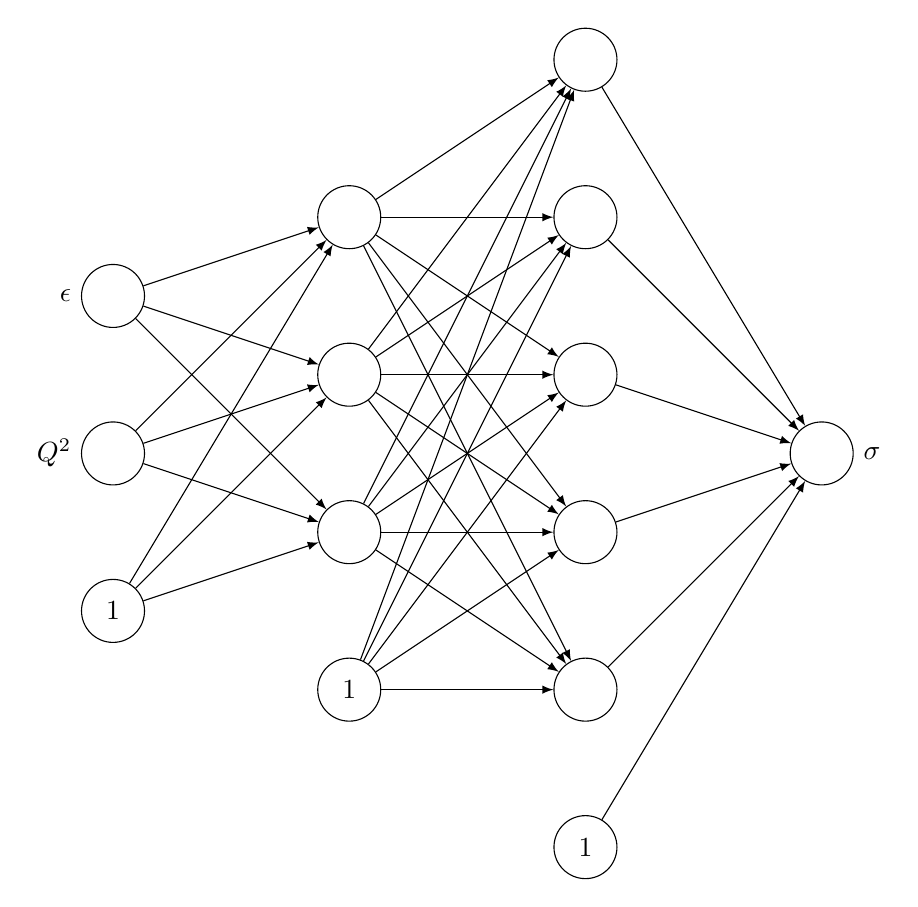
\begin{tikzpicture}
		[   cnode/.style={draw=black,draw=black,fill=#1,minimum width=8mm,circle},
		]
		\tikzset{normal arrow/.style={draw,-latex}}
		\node[cnode=white,label=0:$\sigma$] (s) at (9,-7) {};
		
		\node[cnode=white,label=180:] (x-3) at (0,-9) {1};
		
		
		\node[cnode=white,label=180:] (p-4) at (3,-10) {$1$};
		
		\node[cnode=white,label=180:] (z-6) at (6,-12) {$1$};	
		
		
		\node[cnode=white,label=180:$\epsilon$] (x-1) at (0,-5) {};
		\node[cnode=white,label=180:$Q^2$] (x-2) at (0,-7) {};
		
		\node[cnode=white,label=180:] (p-1) at (3,-4) {};
		\node[cnode=white,label=180:] (p-2) at (3,-6) {};
		\node[cnode=white,label=180:] (p-3) at (3,-8) {};
		
		\node[cnode=white,label=180:] (z-1) at (6,-2) {};
		\node[cnode=white,label=180:] (z-2) at (6,-4) {};
		\node[cnode=white,label=180:] (z-3) at (6,-6) {};
		\node[cnode=white,label=180:] (z-4) at (6,-8) {};
		\node[cnode=white,label=180:] (z-5) at (6,-10) {};
		
		
		
		\foreach \x in {1,...,6}
		{
			\path[normal arrow] (z-\x) -- node[above,sloped,pos=0.4] {} (s);
		}
		
		
		\foreach \x in {1,...,3}
		{   
			\foreach \y in {1,...,3}
			{   
				
				\path[normal arrow] (x-\x) -- (p-\y); 				
			}
		}
		
		\foreach \x in {1,...,4}
		{   
			\foreach \y in {1,...,5}
			{   
				
				\path[normal arrow] (p-\x) -- (z-\y); 
			}
			
			\ifnum \x=5
			\path[normal arrow] (z-\x) -- node[above,sloped,pos=0.4] {} (s);
			\else
			
			\fi
		}
		\end{tikzpicture}}
	\caption{Schemat sieci neuronowej zastosowanej w pierwszej analizie, która składa się z: i) warstwy wejściowej z dwoma neuronami, ii) dwóch warstw ukrytych z odpowiednio trzema i pięcioma neuronami, iii) warstwy wyjściowej z jednym neuronem. Linie zakończone strzałką oznaczają wagi odpowiadające każdej z par neuronów} \label{tab:scheme1} 	
\end{SCfigure}


%
%\begin{figure}[hp!]
%	\centering
%	\includegraphics[width=1\textwidth]{eta.eps}
%	\caption{Ewolucja parametrów $\eta_k$ podczas jednego z treningów modelu. W ciągu kolejnych epok, wartości parametrów ustalane na podstawie równania \ref{eq_eta2} zbiegają do wartości bliskich 1.} 
%	\label{fig:eta}
%\end{figure}
%
\begin{figure}[hp!]
	\centering
	\includegraphics[width=1\textwidth]{eta_proba.eps}
	\caption{Ewolucja parametrów $\eta_k$ podczas jednego z treningów modelu. W ciągu kolejnych epok, wartości parametrów ustalane na podstawie równania \ref{eq_eta2} zbiegają do wartości bliskich 1.} 
	\label{fig:eta}
\end{figure}
%
%\begin{figure}[hp!]
%	\centering
%	\includegraphics[width=1\textwidth]{learning_cur.eps}
%	\caption{Zmiana wartości funkcji straty podczas nauki modelu. Wartość funkcji obliczana na podstawie zbioru treningowego oznaczona jest kolorem niebieskim, dla zbioru walidacyjnego - pomarańczowym.} 
%	\label{fig:learning_cur}
%\end{figure}
%
\begin{figure}[hp!]
	\centering
	\includegraphics[width=1\textwidth]{learning_cur_proba.eps}
	\caption{Zmiana wartości funkcji straty podczas nauki modelu. Wartość funkcji obliczana na podstawie zbioru treningowego oznaczona jest kolorem niebieskim, dla zbioru walidacyjnego - pomarańczowym.} 
	\label{fig:learning_cur}
\end{figure}
%
%\begin{figure}[hp!]
%	\centering
%	\includegraphics[width=1\textwidth]{eta_lc.eps}
%	\caption{} 
%	\label{fig:eta}
%\end{figure}
%

\subsubsection{Wyniki}
%
Wyniki wytrenowanych modeli tworzą statystykę, której najważniejszymi parametrami są średnia przedstawiana jako wynik analizy, oraz odchylenie standardowe, które wyznacza zakres bardzo prawdopodobnych wyników, na wykresie przedstawiany jako zacieniowany obszar.
Rysunek \ref{fig:const_q2} przedstawia zależność przekroju czynnego $\sigma\left(\epsilon\right)$, dla kilku ustalonych wartości $Q^2$. Otrzymane funkcje mają przebieg liniowy o bardzo podobnym współczynniku kierunkowym a błąd modelu $1\sigma$ znacznie wzrasta wraz ze wzrostem $Q^2$.
%
%\begin{figure}[htp!]
%	\centering
%	\includegraphics[width=.98\textwidth]{const_q2.eps}
%	\caption{Zależność przekroju czynnego $\sigma$ od czynnika kinematycznego $\epsilon$ przy ustalonym przekazie czteropędu $Q^2$. Linia ciągła wyznacza średnią wartość po wszystkich wytrenowanych sieciach. Kolor szary wyznacza obszar niepewności $1\sigma$.} 
%	\label{fig:const_q2}
%\end{figure}
%
\begin{figure}[htp!]
	\centering
	\includegraphics[width=.98\textwidth]{const_q2_data.eps}
	\caption{Zależność przekroju czynnego $\sigma$ od czynnika kinematycznego $\epsilon$ przy ustalonym przekazie czteropędu $Q^2$. Linia ciągła wyznacza średnią wartość po wszystkich wytrenowanych sieciach. Kolor szary wyznacza obszar niepewności $1\sigma$.} 
	\label{fig:const_q2}
\end{figure}
%
%\begin{figure}[htp!]
%	\centering
%	\includegraphics[width=.98\textwidth]{const_eps.eps}
%	\caption{Zależność przekroju czynnego $\sigma$ od przekazu czteropędu $Q^2$ przy ustalonym czynniku kinematycznym $\epsilon$. Linia ciągła wyznacza średnią wartość po wszystkich wytrenowanych sieciach. Kolor szary wyznacza obszar niepewności $1\sigma$.} 
%	\label{fig:const_eps}
%\end{figure}
%
\begin{figure}[htp!]
	\centering
	\includegraphics[width=.98\textwidth]{const_eps_data.eps}
	\caption{Zależność przekroju czynnego $\sigma$ od przekazu czteropędu $Q^2$ przy ustalonym czynniku kinematycznym $\epsilon$. Linia ciągła wyznacza średnią wartość po wszystkich wytrenowanych sieciach. Kolor szary wyznacza obszar niepewności $1\sigma$.} 
	\label{fig:const_eps}
\end{figure}
%
Zależność przekroju czynnego $\sigma \left(Q^2\right)$ przy ustalonym parametrze $\epsilon$ znajduje się na rysnku \ref{fig:const_eps}. Możemy zauważyć, że im niższa wartość $\epsilon$ tym mniejszy przekrój czynny dla $Q^2=0$, następnie krzywe mają bardzo podobny przebieg, niezależnie od ustalonego parametru $\epsilon$ zbiegają do tej samej maksymalnej wartości $\sigma$ wraz ze wzrostem $Q^2$. Ponadto, wraz ze wzrostem $Q^2$ rośnie niepewność otrzymanego wyniku, dla $Q^2 = 10 \text{ GeV}^2$ obszar błędu modelu $1\sigma$ wynosi aż $\pm 1$.
%
Po zbadaniu podstawowych zależności estymowanej funkcji od kwadratu przekazu czteropędu oraz czynnika kinematycznego wyznaczono elektryczny i magnetyczny funkcji postaci. Wiemy, że  
%
\begin{equation}
\sigma_R(\epsilon, Q^2) =\tau G_{M_p}^2(Q^2) + \epsilon G_{E_p}^2(Q^2),
\end{equation}
%
obliczając pochodną po parametrze $\epsilon$ otrzymamy kwadrat elektrycznej funkcji postaci protonu, więc
%
\begin{equation}
G_{E_p}(Q^2) = \sqrt{\frac{\partial \sigma_R(\epsilon, Q^2)}{\partial \epsilon}}.
\end{equation}
%
Następnie magnetyczna funkcja postaci protonu wyraża się wzorem
%
\begin{equation}
G_{M_p}(Q^2) =   \sqrt{\frac{\sigma_R(\epsilon, Q^2) - \epsilon \frac{\partial \sigma_R(\epsilon, Q^2)}{\partial \epsilon}}{\tau}}
\end{equation}
%
Należy pamiętać, że pochodna $\frac{\partial \sigma_R(\epsilon, Q^2)}{\partial \epsilon}$ musi zostać wyznaczona dla ustalonej wartości czynnika kinematycznego $\epsilon$. Ponieważ przyjmuje on wartość z przedziału $\left[0,1\right]$, pochodną wyznaczano dla $\epsilon$ będących 11 pierwszymi wyrazami ciągu arytmetycznego o przepisie: $\epsilon_n = (n-1) \times 0.1$. Powtarzając te procedurę dla każdego wytrenowanego modelu otrzymujemy $2500 \times 11$ wyników, ich średnia tworzy wynik modelu. Wykresy \ref{fig:ff1} przedstawiają obliczone w ten sposób funkcje postaci protonu. Opisane działanie jest przyczyną niepewności otrzymanego wyniku, która ma dwa źródła. Pierwsze z nich to błąd pochodnej, czyli rozbieżność wyników w zależności od wybranego parametru $\epsilon$ podczas liczenia pochodnej. Drugie z nich spowodowane jest liczbą wytrenowanych modeli, z których każdy przyjmuje nieco inne dane wejściowe, tworzy to dużą statystykę wyników pochodzących ze wszystkich nauczonych modeli.
%
Otrzymane funkcje postaci zostały porównane z przewidywaniami z publikacji \cite{2009PhRvC..79f5204A} i ich graficzne przedstawienie znajduje się na rysunku \ref{fig:ff1}. Wartość funkcji $G_{E_p}\left(Q^2=0\text{ GeV}^2\right)$ powinna wynosić $1$, mimo że wynik modelu jest niedoszacowany to wartość $1$ znajduje się w obszarze niewielkiego błędu. Niestety wraz ze wzrostem $Q^2$ wzrasta rozbieżność między porównywanymi funkcjami, dla $Q^2 \simeq 2.0\text{ GeV}^2$ obserwujemy nienaturalną zmianę wypukłości funkcji, której się niespodziewamy, i która nie występuje w wyniku z \cite{2009PhRvC..79f5204A}. Jest to jedyny obszar, w którym porównywana funkcja znajduje się po za obszarem niepewności modelu $2\sigma$. Przebieg magnetycznej funkcji postaci $G_{M_p}$ charakteryzuje się bardzo dużą niepewnością w rejonach niskiej wartości $Q^2$, mimo to średni wynik jest bliski pożądanej wartości bliskiej 1. Powyżej wartości $Q^2 \simeq 0.2\text{ GeV}^2$ niepewność pomiaru znacznie się zmniejsza, porównywany rezultat znajduje się na granicy niepewności $2\sigma$ różniąc się od wyniku modelu o stałą wartość około $0.05$, modele zaczynają się znacznie różnić dopiero dla wartości $Q^2$ przekraczajączych $10 \text{ GeV}^2$. Całkowity rezultat należy jednak ocenic pozytywnie, porównywana funkcja rzadko znajduje się po za obszarem niepewności modelu $2\sigma$. 

%Wyniki przedstawione zostały na rysunkach \ref{fig:ge1} oraz \ref{fig:gm1}. 

% $\left[0,0; 0,1; 0,2; 0,3; 0,4; 0,5; 0,6; 0,7; 0,8; 0,9; 1,0 \right]$ 
%Dla każdego z 2500 wytrenowanych modeli została wyznaczona zależność $G_{Ep}$ i $G_{Mp}$ od $Q^2$ d Linia ciągła opisana jako wynik działania modelu przedstawia średni wyni

%
%\begin{figure}
%	\centering
%	\begin{subfigure}[b]{1\textwidth}
%		\includegraphics[width=1.1\linewidth]{ge_.eps}
%		\caption{}
%		\label{fig:ge1} 
%	\end{subfigure}
	
%	\begin{subfigure}[b]{1\textwidth}
%		\includegraphics[width=1.1\linewidth]{gm_.eps}
%		\caption{}
%		\label{fig:gm1}
%	\end{subfigure}
	
%	\caption{Elektryczna (a) i magnetyczna (b) funkcja postaci. Linia ciągła przedstawia średnią ze wszystkich modeli, zacieniowane regiony wyznaczają obszary $1\sigma$ powstałe z dwóch różnych przyczyn. Jasnoszary obszar opisany jako błąd modelu to odchylenie standardowe opisujące rozkład wyników wszystkich wytrenowanych modeli. Ciemnoszary obszar wyznacza odchylenie standardowe opisujące rozkład wyników powstałych na skutek obliczeń pochodnej dla różnych wartości $\epsilon$ z zakresu $[0,1]$. Przerywana linia to wyniki przedstawione w \cite{2009PhRvC..79f5204A}.}
%\end{figure}
%
\begin{figure}[htp!]
	\centering
	\includegraphics[width=1.15\textwidth]{anl_1_.eps}
	\caption{Elektryczna (a) i magnetyczna (b) funkcja postaci. Linia ciągła przedstawia średnią ze wszystkich modeli, zacieniowane regiony wyznaczają obszary $1\sigma$ powstałe z dwóch różnych przyczyn. Jasnoszary obszar opisany jako błąd modelu to odchylenie standardowe opisujące rozkład wyników wszystkich wytrenowanych modeli. Ciemnoszary obszar wyznacza odchylenie standardowe opisujące rozkład wyników powstałych na skutek obliczeń pochodnej dla różnych wartości $\epsilon$ z zakresu $[0,1]$. Przerywana linia to wyniki przedstawione w \cite{2009PhRvC..79f5204A}.}
	\label{fig:ff1}
\end{figure}

\newpage

\section{Analiza nr 2}

Celem drugiej analizy jest modelowanie elektrycznego i magnetycznego czynnika postaci przy wykorzystaniu danych przekrojów czynnych rozpraszania elektron-proton oraz pomiarów eksperymentalnych stosunku funkcji postaci.

%
Dane wejściowe w następnej analizie to 450 punktów pomiarowych analizowanych w pierwszej analizie powiększone o zbiór 68 pomiarów stosunku funkcji postaci $G_{E_p}/G_{M_p}$ wraz z niepewnością pomiarową w zależności od kwadratu przekazu czteropędu $Q^2$. Ponieważ znamy jeden z więzów stosunku funkcji postaci, do zbioru dodany został 69 i 70 punkt: $\mathcal{R}\left(Q^2 = 0 \text{ GeV}^2\right) = 1$, $\Delta \mathcal{R} = 0,001$. Razem otrzymujemy 520 pomiarów co sugeruje wybranie parametru \textit{k}-krotnej walidacji jako $k=5$.
%
Wykorzystana podczas nauki drugiego modelu funkcja straty $\chi^2$ (\ref{eq_loss2}) jest modyfikacją funkcji wykorzystanej w pierwszej analizie. Do użytej wcześniej funkcji błędu dodany został składnik (\ref{eq_rat}) uwzględniający błąd estymacji stosunku $\mathcal{R} = G_{E_p}/G_{M_p}$ oraz składniki dbające o zachowanie więzów $G_{E_p}\left(Q^2=0\text{ GeV}^2\right) = 1$, $G_{M_p}\left(Q^2=0\text{ GeV}^2\right) = 1$ - równanie (\ref{eq_ge_gm}).
%
\begin{equation}
\chi^2 = \frac{1}{n} \left[ \chi_{\sigma}^2 + \chi_{PT}^2 + \chi_{G_M}^2  + \chi_{G_E}^2  \right], \label{eq_loss2}
\end{equation}
%
\begin{equation}
\chi_{PT}^2 = \sum_{i=1}^{n_k^{PT}} \left( \frac{\mathcal{R}_i^{th} - \mathcal{R}_i^{ex}}{\Delta \mathcal{R}_{i}} \right)^2, \label{eq_rat}
\end{equation}

\begin{equation}
\chi_{G}^2 =  \left( \frac{G^{th} - 1}{\Delta G} \right)^2, \label{eq_ge_gm}
\end{equation}
%
gdzie $n_k^{PT}$ to liczba pomiarów stosunków funkcji postaci, $\mathcal{R}_i^{ex}$ to $i$-ty pomiar zmierzony dla odpowiadającej wartości $Q_i^2$, z niepewnością pomiaru $\Delta \mathcal{R}_{i}$ i $\mathcal{R}_i^{th}$ to estymowana przez model wartość. $\chi_{G}^2 = \chi_{G_{E_p}}^2$ lub $\chi_{G_{M_p}}^2 $, natomiast $G^{th} = {G_{E_p}}^{th}\left(Q^2=0\text{ GeV}^2\right)$ lub ${G_{M_p}}^{th}\left(Q^2=0\text{ GeV}^2\right)$ oraz $\Delta {G} = 0,001$. Dane wejściowe służące do treningu sieci zostały ponownie ustandaryzowane analogicznie do procedury przeprowadzonej w pierwszej analizie.


Wynikiem działania sieci neuronowej o dwóch wartstwach ukrytych i hiparametrach przedstawionych w Tabeli \ref{tab:hyper2} są funkcje postaci $G_{Mp}$ oraz $G_{Ep}$ w zależności od zmiennej $Q^2$. Rysunek \ref{tab:scheme2} przedstawia schemat wykorzystanej sieci. Podczas treningu elementy ze zbioru parametrów $\eta_k$ aktualizowane są podczas każdej epoki zgodnie z wzorem \ref{eq_eta2} i ponownie dążą do wartości bliskich 1, przykładowe wartości będące wynikiem nauki modelu znajdują się w Tabeli \ref{tab:etak}. Łącznie zostało wytrenowanych 2500 ($N_{rep} \times k$) modeli. 
%
\begin{SCfigure}[][h]
	\centering
	\resizebox{8.cm}{!}{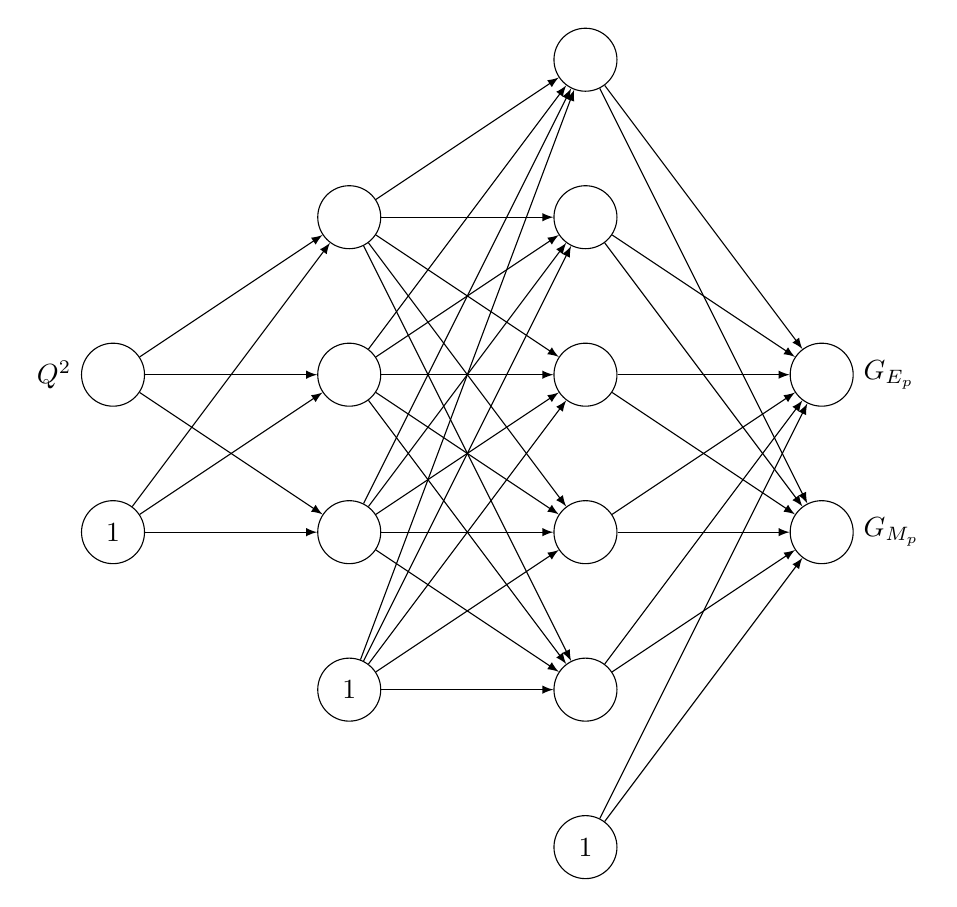
\begin{tikzpicture}
		[   cnode/.style={draw=black,draw=black,fill=#1,minimum width=8mm,circle},
		]
		\tikzset{normal arrow/.style={draw,-latex}}
		\node[cnode=white,label=0:$G_{E_p}$] (s) at (9,-6) {};
		\node[cnode=white,label=0:$G_{M_p}$] (s-1) at (9,-8) {};
		
		\node[cnode=white,label=180:\textit{}] (x-2) at (0,-8) {1};
		
		
		\node[cnode=white,label=180:] (p-4) at (3,-10) {$1$};
		
		\node[cnode=white,label=180:] (z-6) at (6,-12) {$1$};	
		
		
		%		\node[cnode=white,label=180:$\epsilon$] (x-1) at (0,-5) {};
		\node[cnode=white,label=180:$Q^2$] (x-1) at (0,-6) {};
		
		\node[cnode=white,label=180:] (p-1) at (3,-4) {};
		\node[cnode=white,label=180:] (p-2) at (3,-6) {};
		\node[cnode=white,label=180:] (p-3) at (3,-8) {};
		
		\node[cnode=white,label=180:] (z-1) at (6,-2) {};
		\node[cnode=white,label=180:] (z-2) at (6,-4) {};
		\node[cnode=white,label=180:] (z-3) at (6,-6) {};
		\node[cnode=white,label=180:] (z-4) at (6,-8) {};
		\node[cnode=white,label=180:] (z-5) at (6,-10) {};
		
		
		
		\foreach \x in {1,...,6}
		{
			\path[normal arrow] (z-\x) -- node[above,sloped,pos=0.4] {} (s);
			\path[normal arrow] (z-\x) -- node[above,sloped,pos=0.4] {} (s-1);
		}
		
		
		\foreach \x in {1,...,2}
		{   
			\foreach \y in {1,...,3}
			{   
				
				\path[normal arrow] (x-\x) -- (p-\y); 				
			}
		}
		
		\foreach \x in {1,...,4}
		{   
			\foreach \y in {1,...,5}
			{   
				
				\path[normal arrow] (p-\x) -- (z-\y); 
			}
			
			\ifnum \x=5
			\path[normal arrow] (z-\x) -- node[above,sloped,pos=0.4] {} (s);
			\path[normal arrow] (z-\x) -- node[above,sloped,pos=0.4] {} (s-1);
			\else
			
			\fi
		}
		\end{tikzpicture}}
	\caption{Schemat sieci neuronowej zastosowanej w drugiej analizie, która składa się z: i) warstwy wejściowej z dwoma neuronami, ii) dwóch warstw ukrytych z odpowiednio trzema i pięcioma neuronami, iii) warstwy wyjściowej z dwoma neuronami. Linie zakończone strzałką oznaczają wagę odpowiadającą każdej z par neuronów} \label{tab:scheme2} 	
\end{SCfigure}
%
\begin{table}
	\centering
	\caption{Hiperparametry modelu podczas drugiej analizy}\label{tab:hyper2} 
	\begin{tabular}{c|c c c}
		\hline 
		Kategoria & Parametr & Wartość &   \\\hline
		Generowanie danych & $N_{rep}$ & 500 & \\ \hline
		$k$-krotna walidacja krzyżowa & $k$ & 5 &\\ \hline
		
		Algorytm uczący& $\alpha$ (\textit{learning rate}) & 0,02 & \\ 
		& $\lambda$ (\textit{decay}) & 0,001 & \\ 
		& $\beta$ (\textit{pęd}) & 0,9 & \\ \hline
		Sieć neuronowa & Liczba warstw & 2 & \\ 
		& Ilość neuronów & (3,5) & \\ \hline
		
	\end{tabular}
\end{table}

%wartosci parametrow eta
%
\begin{table}
	\centering
	\caption{Przykładowe końcowe wyniki parametrów $\eta_k$ podczas nauki modelu w drugiej analizie}\label{tab:etak} 
	\begin{tabular}{p{2cm}p{5cm}p{2.5cm}p{2.5cm}}
		%{c|c c c}
		\hline 
		L.p & Zbiór danaych & $\Delta \eta_k [\%]$ & $\eta_k$  \\\hline
		1& \texttt{And94\_000.dat}&1,77&1,014\\ \hline
		2& \texttt{And94\_100.dat}&2,70&1,018\\ \hline
		3& \texttt{Arn86\_1500.dat}&3,00&1,017\\ \hline
		4& \texttt{Bar66\_1700.dat}&2,50&0,981\\ \hline
		5& \texttt{Bar73\_200.dat}&2,10&0,971\\ \hline
		6& \texttt{Bar73\_300.dat}&2,10&0,998\\ \hline
		7& \texttt{Bar73\_400.dat}&2,10&0,980\\ \hline
		8& \texttt{Ber71\_700.dat}&4,00&0,947\\ \hline
		9& \texttt{Bor74\_1900.dat}&2,00&0,971\\ \hline
		10& \texttt{Chr03\_500.dat}&1,50&0,959\\ \hline
		11& \texttt{Dut03\_1400.dat}&1,90&0,989\\ \hline
		12& \texttt{Goi70\_1800.dat}&3,80&0,936\\ \hline
		13& \texttt{Jan66\_1600.dat}&1,60&0,965\\ \hline
		14& \texttt{Kir73\_1100.dat}&4,00&1,050\\ \hline
		15& \texttt{Lit67\_600.dat}&4,00&0,941\\ \hline
		16& \texttt{Mur74\_2200.dat}&4,60&1,016\\ \hline
		17& \texttt{Nic99\_1300.dat}&1,90&1,025\\ \hline
		18& \texttt{Pri71\_900.dat}&1,90&1,009\\ \hline
		19& \texttt{Qat05\_2300.dat}&3,00&0,981\\ \hline
		20& \texttt{Sil93\_1000.dat}&3,00&0,997\\ \hline
		21& \texttt{Sim80\_2100.dat}&0,50&1,017\\ \hline
		22& \texttt{Sim81\_2000.dat}&0,50&0,997\\ \hline
		23& \texttt{Ste75\_800.dat}&2,40&0,983\\ \hline
		24& \texttt{Wal94\_1200.dat}&1,90&0,964\\ \hline
	\end{tabular}
\end{table}


\subsubsection{Wyniki}
%
Wyniki nauczonych modeli tworzą statystykę, której najważniejszymi parametrami są średnia przedstawiana jako wynik modelu, oraz odchylenie standardowe, które wyznacza zakres bardzo prawdopodobnych wyników, na wykresie przedstawiany jako zacieniowany obszar. Rysunek \ref{fig:ff2} przedstawia wykresy otrzymanych funkcji postaci protonu. Lewa część obrazka przedstawia magnetyczną funkcję postaci protonu w zależności od kwadratu przekazu czteropędu $G_{M_p}\left(Q^2\right)$, prawa część rysunku przedstawia przebieg elektrycznej funkcji postaci $G_{E_p}\left(Q^2\right)$. Otrzymane wyniki są znacznie bliższe przebiegom funkcji z publikacji \cite{2009PhRvC..79f5204A} i prawie całkowicie mieszczą się w zaznaczonych ciemnym kolorem obszarach $\pm 2\sigma$. Wariancja magnetycznej funkcji postaci jest w przybliżeniu stały na całej długości przedstawionego przebiegu funkcji i wynosi około $0.015$, odchylenie standardowe dla elektrycznej funkcji postaci w pobliżu $Q^2 \rightarrow 0$ jest bardzo niewielkie i znacznie wzrasta wraz z $Q^2$ osiągając wysoką wartość $0.1$. Może to być spowodowane mniejszą ilością pomiarów doświadczalnych dla dużych wartości $Q^2$.
% 
\begin{figure}[hp!]
	\centering
	\includegraphics[width=1.\textwidth]{anl_2.eps}
	\caption{Magnetyczna i elektryczna funkcja postaci. Linia ciągła oznacza średnią ze wszystkich modeli, zacienione pola wyznaczają obszary $1 \sigma$ (jasny) oraz $2\sigma$ (ciemny). Linia przerywana przedstawia wyniki z publikacji \cite{2009PhRvC..79f5204A}. } 
	\label{fig:ff2}
\end{figure}
% 
Najbardziej zauważalna różnica pomiędzy funkcjami występuje dla wartości $Q^2 \simeq 0.15 \text{ GeV}^2$, wynik modelu zarówno dla $G_{M_p}$ jak i dla $G_{E_p}$ jest przeszacowany względem przerywanej krzywej. Porównywana elektryczna funkcja postaci w tym obszarze nieznacznie wychodzi po za pokazany obszar niepewności modelu. 
Dodatkowym źródłem danych służącym do nauki sieci neuronowej w stosunku do poprzedniego modelu były dane zawierające eksperymentalne pomiary stosunków elektrycznej i magnetycznej funkcji postaci w zależności do kwadratu przekazu czteropędu. Rysunek \ref{fig:ratio2} przedstawia wspomniane powyżej pomiary wraz z zaznaczoną ich niepewnością. Ponadto przerywaną linią zaznaczono dopasowanie liniowe, które dobrze opisuje relację pomiędzy funkcjami postaci oraz wynik modelu wraz z odchyleniami standardowymi. Iloraz $\mu G_{E_p} / G_{M_p}$ szczególnie dobrze opisywany jest przez model dla niewielkich wartości $Q^2$ i cechuje się w tym obszarze bardzo niewieką niepewnością. Wraz ze wzrostem $Q^2$ rezultat modelu jest coraz mniej liniowy, $G_{E_p}$ staje się przeszacowane, a odchylenie standardowe znacznie wzrasta. Większość pomiarów doświadczalnych pozostaje jednak w obszarze niepewności $-2\sigma$.
%
\begin{figure}[hp!]
	\centering
	\includegraphics[width=1.\textwidth]{ratio_2.eps}
	\caption{Pomiary stosunku elektrycznej i magnetycznej funkcji postaci wraz z dopasowaniem liniowym oraz dopasowaniem modelu statystycznego. Linia ciągła oznacza średni wynik ze wszystkich wytrenowanych modeli, zacienione pola wyznaczają obszary $1 \sigma$ oraz $2\sigma$.} 
	\label{fig:ratio2}
\end{figure}

\newpage

\section{Analiza nr 3}

Celem trzeciej analizy oprócz modelowania elektrycznego i magnetycznego czynnika postaci jest przewidywanie wartości poprawki dwu-fotonowej przy wykorzystaniu danych przekrojów czynnych rozpraszania elektron-proton oraz pomiarów eksperymentalnych stosunku funkcji postaci.

%
Wykorzystane podczas analizy dane składają sie z dwóch zestawów. Pierwszy to 450 punktów pomiarowych przekrojów czynnych, których wartości zostały zmodyfikowane o poprawkę TPE. Struktura danych wejściowych jest analogiczna do tych wykorzystywanych w powyższych analizach - cztery kolumny zawierają zmienną objaśnianą $\sigma$ , niepewność pomiaru przekroju czynnego $\Delta \sigma$ i dwie zmienne objaśniające $Q^2$ oraz $\epsilon$. Drugi zestaw to 70 pomiarów doświadczalnych stosunków funkcji postaci $G_{E_p} / G_{M_p}$ wraz z niepewnością pomiarową w zależności od kwadratu czteropędu $Q^2$. Razem otrzymujemy 520 pomiarów co ponownie sugeruje wybranie parametru \textit{k}-krotnej walidacji jako $k=5$. Zastosowana podczas nauki trzeciego modelu funkcja straty $\chi^2$ (\ref{eq_loss3}) składa się się z tych samych składników co funkcja wykorzystana podczas drugiej analizy (\ref{eq_loss2}), jednak do całkowitego przekroju czynnego należy dodać poprawkę zależną od kwadratu przekazu czteropędu $Q^2$ i czynnika kinematycznego $\epsilon$ jak przedstawiono w równaniu \ref{eq:sigma_c2}. Dane wejściowe służące do treningu sieci zostały ponownie ustandaryzowane, wraz z inicjalizacją wag zostały wykonane identycznie jak w poprzednich analizach.
%
\begin{equation}
\sigma_R(\epsilon, Q^2) =\tau G_{M_p}^2(Q^2) + \epsilon G_{E_p}^2(Q^2) + \Delta C_{2 \gamma} \left(Q^2, \epsilon \right), \label{eq:sigma_c2}
\end{equation}
%
\begin{equation}
\chi^2 = \frac{1}{n} \left[ \chi_{\sigma}^2 + \chi_{PT}^2 + \chi_{G_M}^2  + \chi_{G_E}^2  \right]. \label{eq_loss3}
\end{equation}


Podczas analizy na szczególną uwagę zasługuję struktura sieci neuronowej przedstawiona na rysunku \ref{tab:scheme3}. Wynikiem działania sieci są funkcje postaci $G_{M_p}$ oraz $G_{E_p}$ w zależności od $Q^2$ oraz poprawka $\Delta C_{2\gamma}$ zależna od $Q^2$ i $\epsilon$, takie wymagania wymuszają przerwanie połączeń między niektórymi neuronami. Sieć składa się z warstwy wejściowej, dwóch warstw ukrytych oraz warstwy wyjściowej, wejściowa składa się z dwóch neuronów $(Q^2, \epsilon)$. Pierwsza warstwa ukryta zawiera trzy neurony połączone wyłącznie z $Q^2$ oraz jeden połączony wyłącznie z $\epsilon$ (3-1). Druga warstwa ukryta to pięć neuronów, ponownie trzy z nich połączone są z neuronami łączącymi się wyłącznie z kwadratem przekazu czteropędu, pozostałe dwa połączone są z neuronem z poprzedniej warstwy połączonym z czynnikiem kinematycznym (3-2). Ostatnia warstwa wyjściowa składa się z trzech neuronów, dwie funkcje postaci otrzymują sygnał pochądzący z trzech neuronów przekazujących sygnał zależny od wartości $Q^2$ natomiast poprawka $\Delta C_{2\gamma}$ połączona jest ze wszystkimi neuronami w poprzedniej warstwie, zatem jej wartości są zależne zarówno od $Q^2$ i $\epsilon$. 

Konstrukcja takiej struktury sieci neuronowej w Kerasie jest nietrywialna, aby uzyskać opisany powyżej efekt skorzystano z warstw Lambda, które umożliwiają wykonywanie operacji arytmetycznych przez warstwy sieci w obrębie zdefiniowanej funkcji lambda. W tej konstrukcji każdy z neuronów wybranej warstwy ukrytej jest zdefiniowany jako warstwa Lambda. Operacje wykonywane na tensorach zdefiniowane jako funkcja lambda pozwalają wybrać, które neurony z warstwy poprzedzającej są wejściem. Następnie wszystkie wybrane neurony zdefiniowane wcześniej jako osobne warstwy łączone są w jedną warstwę - warstwę ukrytą, w której neurony mają zdefiniowane przez nas wejścia. Kolejne warstwy tworzone są w analogiczny sposób. Appendix zawiera szczegóły implementacyjne stworzonego modelu. Tabela \ref{tab:hyper3} przedstawia wykorzystane hiperparametry sieci neuronowej. 

\begin{SCfigure}[][h]
	\centering
	\resizebox{8.cm}{!}{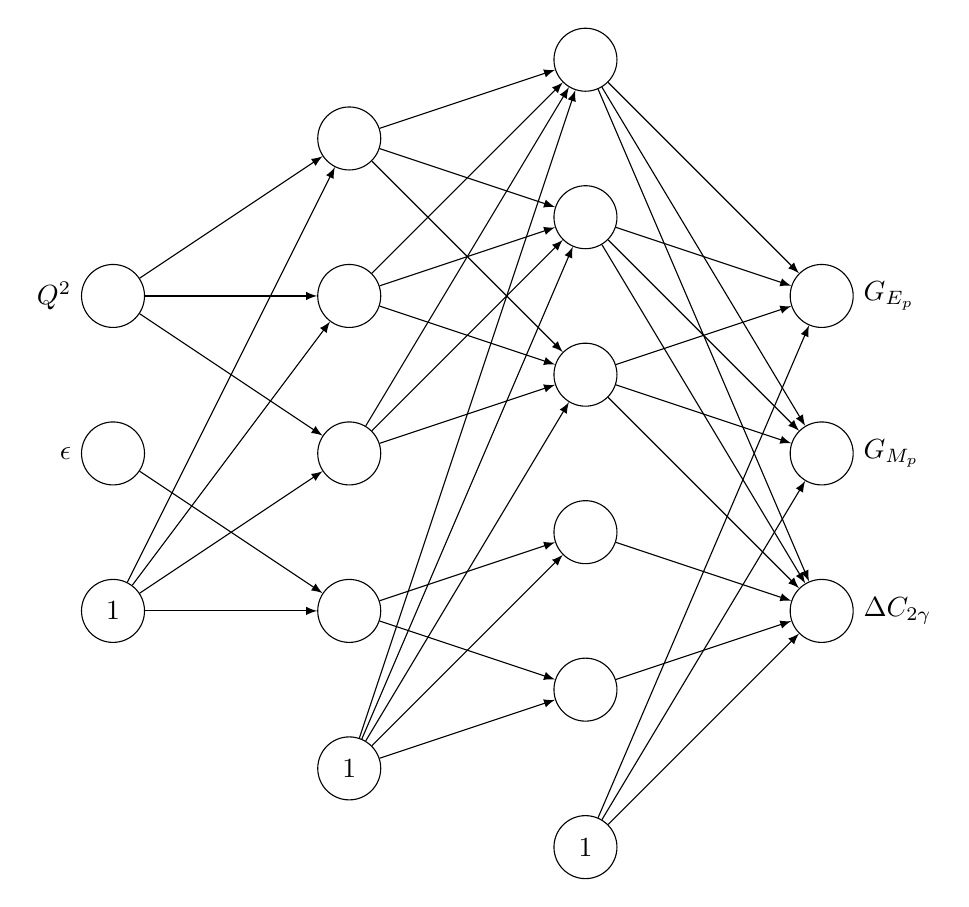
\begin{tikzpicture}
		[   cnode/.style={draw=black,draw=black,fill=#1,minimum width=8mm,circle},
		]
		\tikzset{normal arrow/.style={draw,-latex}}
		\node[cnode=white,label=0:$G_{E_p}$] (s) at (9,-5) {};
		\node[cnode=white,label=0:$G_{M_p}$] (s-1) at (9,-7) {};
	    \node[cnode=white,label=0:$\Delta C_{2\gamma}$] (s-2) at (9,-9) {};
		
		\node[cnode=white,label=180:\textit{}] (x-3) at (0,-9) {1};
		
		
		\node[cnode=white,label=180:] (p-5) at (3,-11) {$1$};
		
		\node[cnode=white,label=180:] (z-6) at (6,-12) {$1$};	
		
		
		\node[cnode=white,label=180:$Q^2$] (x-1) at (0,-5) {};
		\node[cnode=white,label=180:$\epsilon$] (x-2) at (0,-7) {};
		
		\node[cnode=white,label=180:] (p-1) at (3,-3) {};
		\node[cnode=white,label=180:] (p-2) at (3,-5) {};
		\node[cnode=white,label=180:] (p-3) at (3,-7) {};
		\node[cnode=white,label=180:] (p-4) at (3,-9) {};
		
		\node[cnode=white,label=180:] (z-1) at (6,-2) {};
		\node[cnode=white,label=180:] (z-2) at (6,-4) {};
		\node[cnode=white,label=180:] (z-3) at (6,-6) {};
		\node[cnode=white,label=180:] (z-4) at (6,-8) {};
		\node[cnode=white,label=180:] (z-5) at (6,-10) {};
		
				
		\foreach \y in {1,...,3}
			{   
				
				\path[normal arrow] (x-1) -- (p-\y); 				
				\path[normal arrow] (x-3) -- (p-\y); 		
				
			}


		\path[normal arrow] (x-2) -- (p-4); 				
		\path[normal arrow] (x-3) -- (p-4); 								


		\foreach \x in {1,...,5}
		{   
			\foreach \y in {1,...,3}
			{   
				\ifnum \x=4
				\else
					\path[normal arrow] (p-\x) -- (z-\y); 
				\fi
			}		
		}
	

		\foreach \x in {4,...,5}
		{   
			\foreach \y in {4,...,5}
			{   
				\path[normal arrow] (p-\x) -- (z-\y); 
			}	
		}	
	
				
		\foreach \x in {1,...,3}
		{
			\path[normal arrow] (z-\x) -- node[above,sloped,pos=0.4] {} (s);
			\path[normal arrow] (z-\x) -- node[above,sloped,pos=0.4] {} (s-1);
			\path[normal arrow] (z-\x) -- node[above,sloped,pos=0.4] {} (s-2);
		}
	
		\foreach \x in {4,...,5}
		{
			\path[normal arrow] (z-\x) -- node[above,sloped,pos=0.4] {} (s-2);
		}
			\path[normal arrow] (z-6) -- node[above,sloped,pos=0.4] {} (s);
			\path[normal arrow] (z-6) -- node[above,sloped,pos=0.4] {} (s-1);
			\path[normal arrow] (z-6) -- node[above,sloped,pos=0.4] {} (s-2);
	
	
	
	
	
		\end{tikzpicture}}
	\caption{Schemat sieci neuronowej zastosowanej w trzeciej analizie, która składa się z: i) warstwy wejściowej z dwoma neuronami, ii) dwóch warstw ukrytych z odpowiednio czterema i pięcioma neuronami, iii) warstwy wyjściowej z trzema neuronami. Linie zakończone strzałką oznaczają wagę odpowiadającą każdej z par neuronów} \label{tab:scheme3} 	
\end{SCfigure}


\begin{table}
	\centering
	\caption{Hiperparametry modelu}\label{tab:hyper3} 
	\begin{tabular}{c|c c c}
		\hline 
		Kategoria & Parametr & Wartość &   \\\hline
		Generowanie danych & $N_{rep}$ & 500 & \\ \hline
		$k$-krotna walidacja krzyżowa & $k$ & 5 &\\ \hline
		
		Algorytm uczący& $\alpha$ (\textit{learning rate}) & 0,02 & \\
		& $\lambda$ (\textit{decay}) & 0,001 & \\ 
		& $\beta$ (\textit{pęd}) & 0,9 & \\ \hline
		Sieć neuronowa & Liczba warstw & 2 & \\ 
		& Ilość neuronów & ((3-1),(3-2)) & \\ \hline
		
	\end{tabular}
\end{table}


\subsubsection{Wyniki}
%
%

Rysunek \ref{fig:ff3} przedstawia wykresy otrzymanych funkcji postaci protonu. Lewa część obrazka przedstawia magnetyczną funkcję postaci protonu w zależności od kwadratu przekazu czteropędu $G_{M_p}\left(Q^2\right)$, prawa część rysunku przedstawia przebieg elektrycznej funkcji postaci $G_{E_p}\left(Q^2\right)$. Otrzymane wyniki zostały ponownie porównywane są z rezultatami publikacji \cite{2009PhRvC..79f5204A}, które całkowicie zawierają się w obszarze $\pm 2\sigma$ otrzymanych wyników. W przypadku magnetycznej funkcji postaci główna różnica to brak zmiany monotoniczności funkcji będącej wynikiem modelu, w okolicach $Q^2 \simeq 0.15 \text{ GeV}^2$ oraz późniejsze niedoszacowanie względem porównywanej funkcji, nie przekraczające różnicy 0.02. Elektryczna funkcja postaci również pozbawiona jest pierwszego niewielkiego przecięcia, następnie spadek wartości zaczyna się wcześniej, tzn. dla nieco mniejszej wartości $Q^2$, jednak jest on mniej gwałtowny. Odchylenie standardowe magnetycznej funkcji postaci jest w przybliżeniu stałe na całej długości przedstawionego przebiegu funkcji i wynosi około $0.01$, wariancja elektrycznej funkcji postaci w pobliżu $Q^2 \rightarrow 0$ jest bardzo niewielka i znacznie wzrasta wraz z $Q^2$.
% 
\begin{figure}[h]
	\centering
	\includegraphics[width=1.\textwidth]{anl_3.eps}
	\caption{Magnetyczna i elektryczna funkcja postaci. Linia ciągła oznacza średnią ze wszystkich modeli, zacienione pola wyznaczają obszary $1 \sigma$ (jasny) oraz $2\sigma$ (ciemny). Linia przerywana przedstawia wyniki z publikacji \cite{2009PhRvC..79f5204A}. } 
	\label{fig:ff3}
\end{figure}

Rysunek \ref{fig:ratio3} przedstawia pomiary eksperymentalne stosunku funkcji postaci wraz z zaznaczoną niepewnością pomiarow, przerywaną linią zaznaczono dopasowanie liniowe oraz wynik modelu wraz z odchyleniami standardowymi. Iloraz $\mu G_{E_p} / G_{M_p}$ szczególnie dobrze opisywany jest przez model dla niewielkich wartości $Q^2$ i cechuje się w tym obszarze bardzo niewieką niepewnością. Wraz ze wzrostem $Q^2$ maleje gęstość pomiarów, $G_{E_p}$ staje się przeszacowane, a odchylenie standardowe znacznie wzrasta. Większość pomiarów doświadczalnych znajduje się jednak w obszarze niepewności $\pm2\sigma$.
%
\begin{figure}[h!]
	\centering
	\includegraphics[width=1\textwidth]{ratio_3.eps}
	\caption{Pomiary stosunku elektrycznej i magnetycznej funkcji postaci wraz z dopasowaniem liniowym oraz dopasowaniem modelu statystycznego. Linia ciągła oznacza średni wynik ze wszystkich wytrenowanych modeli, zacienione pola wyznaczają obszary $1 \sigma$ oraz $2\sigma$.} 
	\label{fig:ratio3}
\end{figure}
%

\begin{figure}[h!]
	\centering
	\includegraphics[width=0.95\textwidth]{c2_q2.eps}
	\caption{Poprawka dwu-fotonowa w zależności od $Q^2$, ciągła linia to wynik modelu, kolory szarne oznaczją odchylenie standardowe $1\sigma$ oraz $2\sigma$.} 
	\label{fig:c2}
\end{figure}

Jednym z wyników sieci nieuwzględnionym podczas wcześniejszych analiz jest poprawka TPE $\Delta C_{2\gamma}$, rysunek \ref{fig:c2} przedstawia jej zależność od kwadratu przekazu czteropędu dla $\epsilon$ będących 11 pierwszymi wyrazami ciągu arytmetycznego o przepisie: $\epsilon_n = (n-1) \times 0.1$. Dla wartości $Q^2 < 1 \text{ GeV}^2$ poprawka ma niewielką wartość i niewielkie odchylenie standardowe, zatem ma niewielki wpływ na wartość całkowitego przekroju czynnego.  Dla $Q^2 > 1 \text{ GeV}^2$ jej średnia wartość zaczyna rosnąć wraz z $Q^2$ do około 0.3, odchylenie standardowe również gwałtownie wzrasta i osiąga wartość około 0.2.


\newpage

\section{Analiza nr 4}

Celem czwartej analizy jest uzyskanie przewidywań wyników o jak największym znaczeniu fizycznym. Oznacza to, że oprócz elektrycznego i magnetycznego czynnika postaci modelowana jest także wartość poprawki TPE wraz z uwzględnieniem teoretycznych więzów wszystkich składników całkowitego przekroju czynnego elastycznego rozpraszania elektron-proton. Analiza jest pod wieloma względami przeprowadzona analogicznie do analizy nr 3, tym razem jednak odpowiedź sieci została zmodyfikowana w taki sposób aby wymusić na wynikach otrzymanie znanych więzów funkcji postaci w punkcie $Q^2 = 0$  i poprawki TPE dla $\epsilon=1$, o więzach przypominają poniższe równania

\begin{eqnarray}
&G_{E_p}(Q^2 = 0) &= 1, \\
&G_{M_p}(Q^2 = 0)/ \mu_p &= 1, \\
&\Delta C_{2 \gamma}(\epsilon=1) &= 0. 
\end{eqnarray}
%(\ref{eq:constraints})

Aby to uzyskać wykorzystano metodę opisaną w pracy \cite{2014PhRvC..90e4334G}. Wynikiem działania sieci neuronowej są funkcje oznaczone jako $o_{E_p}$, $o_{M_p}$, $ o_{2 \gamma}$, które następnie przekształcane są do funkcji postaci $G_{E_p}$, $G_{M_p}$ oraz poprawki TPE $\Delta C_{2 \gamma}$ zgodnie z poniższymi równaniami

\begin{eqnarray}
&G_{E_p} &= \left(1-Q^2o_{E_p}\right) G_D,\\
&G_{M_p}/ \mu_p &= \left(1-Q^2  o_{M_p}\right) G_D,\\
&\Delta C_{2 \gamma} &= \left(1-\epsilon \right) o_{2 \gamma} G_D.
\end{eqnarray}


\begin{SCfigure}[][h]
	\centering
	\resizebox{9cm}{!}{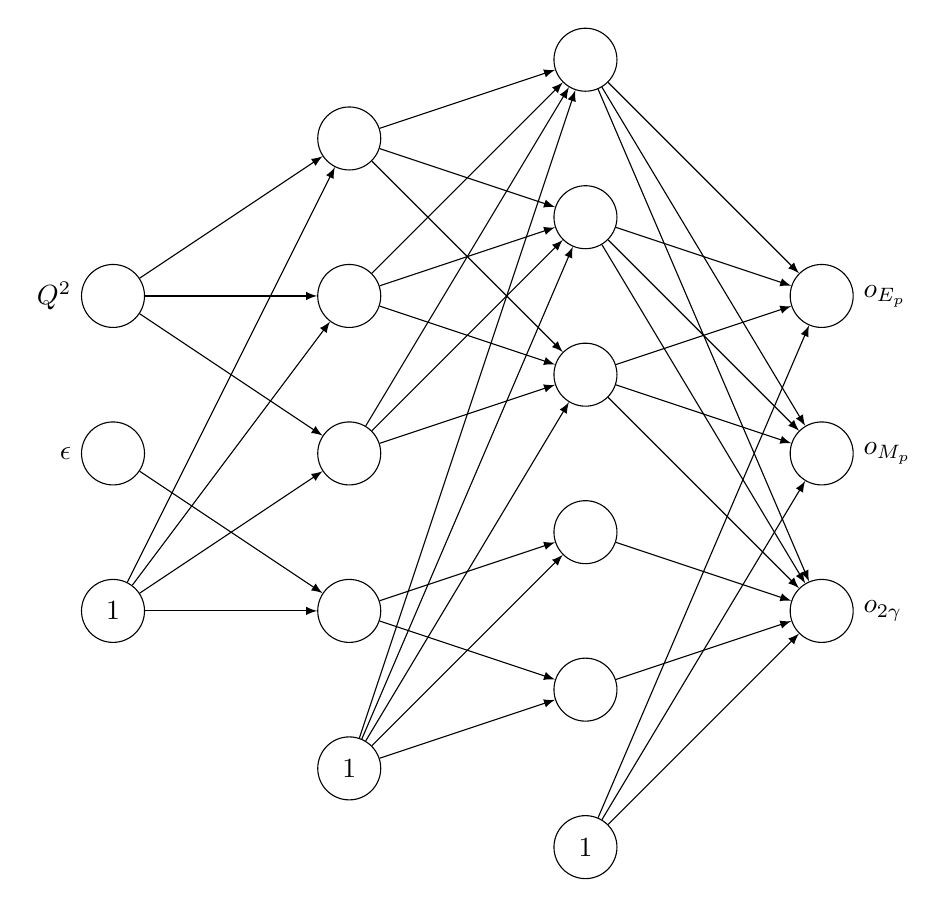
\begin{tikzpicture}
		[   cnode/.style={draw=black,draw=black,fill=#1,minimum width=8mm,circle},
		]
		\tikzset{normal arrow/.style={draw,-latex}}
		\node[cnode=white,label=0:$o_{E_p}$] (s) at (9,-5) {};
		\node[cnode=white,label=0:$o_{M_p}$] (s-1) at (9,-7) {};
		\node[cnode=white,label=0:$o_{2\gamma}$] (s-2) at (9,-9) {};
		
		\node[cnode=white,label=180:\textit{}] (x-3) at (0,-9) {1};
		
		
		\node[cnode=white,label=180:] (p-5) at (3,-11) {$1$};
		
		\node[cnode=white,label=180:] (z-6) at (6,-12) {$1$};	
		
		
		\node[cnode=white,label=180:$Q^2$] (x-1) at (0,-5) {};
		\node[cnode=white,label=180:$\epsilon$] (x-2) at (0,-7) {};
		
		\node[cnode=white,label=180:] (p-1) at (3,-3) {};
		\node[cnode=white,label=180:] (p-2) at (3,-5) {};
		\node[cnode=white,label=180:] (p-3) at (3,-7) {};
		\node[cnode=white,label=180:] (p-4) at (3,-9) {};
		
		\node[cnode=white,label=180:] (z-1) at (6,-2) {};
		\node[cnode=white,label=180:] (z-2) at (6,-4) {};
		\node[cnode=white,label=180:] (z-3) at (6,-6) {};
		\node[cnode=white,label=180:] (z-4) at (6,-8) {};
		\node[cnode=white,label=180:] (z-5) at (6,-10) {};
		
		
		\foreach \y in {1,...,3}
		{   
			
			\path[normal arrow] (x-1) -- (p-\y); 				
			\path[normal arrow] (x-3) -- (p-\y); 		
			
		}
		
		
		\path[normal arrow] (x-2) -- (p-4); 				
		\path[normal arrow] (x-3) -- (p-4); 								
		
		
		\foreach \x in {1,...,5}
		{   
			\foreach \y in {1,...,3}
			{   
				\ifnum \x=4
				\else
				\path[normal arrow] (p-\x) -- (z-\y); 
				\fi
			}		
		}
		
		
		\foreach \x in {4,...,5}
		{   
			\foreach \y in {4,...,5}
			{   
				\path[normal arrow] (p-\x) -- (z-\y); 
			}	
		}	
		
		
		\foreach \x in {1,...,3}
		{
			\path[normal arrow] (z-\x) -- node[above,sloped,pos=0.4] {} (s);
			\path[normal arrow] (z-\x) -- node[above,sloped,pos=0.4] {} (s-1);
			\path[normal arrow] (z-\x) -- node[above,sloped,pos=0.4] {} (s-2);
		}
		
		\foreach \x in {4,...,5}
		{
			\path[normal arrow] (z-\x) -- node[above,sloped,pos=0.4] {} (s-2);
		}
		\path[normal arrow] (z-6) -- node[above,sloped,pos=0.4] {} (s);
		\path[normal arrow] (z-6) -- node[above,sloped,pos=0.4] {} (s-1);
		\path[normal arrow] (z-6) -- node[above,sloped,pos=0.4] {} (s-2);
		
		
		
		
		
		\end{tikzpicture}}
	\caption{Schemat sieci neuronowej zastosowanej w czwartej analizie, struktura jest bliźniacza do sieci zastosowanej w trzeciej analizie jednak neurony w warstwie wyjściowej modelu zmieniły się na: $o_{E_p}$, $o_{M_p}$ i $o_{2\gamma}$ } \label{tab:scheme4} 	
\end{SCfigure}

%
Schemat wykorzystanej sieci został przedstawiony na rysunku \ref{tab:scheme4}, warto zwrócić uwagę, że ponownie sieć została tak ustrukturyzowana, że funkcje postaci $G_{E_p}$, $G_{M_p}$ zależne są tylko od $Q^2$, natomiast poprawka $\Delta C_{2\gamma}$ połączona jest ze wszystkimi neuronami w poprzedniej warstwie, zatem jej wartości są zależne zarówno od $Q^2$ i $\epsilon$. Ostatnia analiza wykorzystuje zestaw danych przygotowany do przeprowadzenia analizy nr 3, co ponownie sugeruje wybranie parametru \textit{k}-krotnej walidacji jako $k=5$. Zastosowana podczas nauki czwartego modelu funkcja straty $\chi^2$ (\ref{eq_loss3}) także się nie zmieniła, jedyną zmianą jest wspomniane wcześniej przekształcenie wyniku sieci neuronowej do postaci funkcji $G_{E_p}$, $G_{M_p}$, $\Delta C_{2 \gamma}$. Hiperparametry modelu zostały przedstawione w tabeli \ref{tab:hyper4}.
%

\begin{table}[h]
	\centering
	\caption{Hiperparametry modelu}\label{tab:hyper4} 
	\begin{tabular}{c|c c c}
		\hline 
		Kategoria & Parametr & Wartość &   \\\hline
		Generowanie danych & $N_{rep}$ & 500 & \\ \hline
		$k$-krotna walidacja krzyżowa & $k$ & 5 &\\ \hline
		
		Algorytm uczący& $\alpha$ (\textit{learning rate}) & 0,025 & \\
		& $\lambda$ (\textit{decay}) & 0,002 & \\ 
		& $\beta$ (\textit{pęd}) & 0,9 & \\ \hline
		Sieć neuronowa & Liczba warstw & 2 & \\ 
		& Ilość neuronów & ((3-1),(3-2)) & \\ \hline
		
	\end{tabular}
\end{table}

\subsubsection{Wyniki}
% 
Rysunek \ref{fig:ff4} przedstawia wykresy otrzymanych funkcji postaci protonu. Lewa część obrazka przedstawia magnetyczną funkcję postaci protonu w zależności od kwadratu przekazu czteropędu $G_{M_p}\left(Q^2\right)$, prawa część rysunku przedstawia przebieg elektrycznej funkcji postaci $G_{E_p}\left(Q^2\right)$. Uzyskane wyniki dowodzą, że udało się otrzymać zadane powyżej więzy funkcji, jednak kształty funkcji postaci w istotny sposób różnią się od rezultatów publikacji \cite{2009PhRvC..79f5204A}. Otrzymana przez model magnetyczna funkcja postaci jest rosnąca oraz znacznie przeszacowana w obszarze niskich wartości $Q^2$ względem referencyjnego przebiegu, który charakteryzuje się zmianą monotoniczności. Dopiero dla wartości argumentu $Q^2 > 0.4 \text{GeV}^2$ referencyjny przebieg magnetycznej funkcji postaci znajduje się w obszarze $\pm 2\sigma$ otrzymanych wyników. Różnice między uzyskaną elektryczną funkcją postaci pronu i porównywaną funkcją ponownie najbardziej zauważalne są dla stosunkowo niewielkich wartości $Q^2$. Wynik ponownie pozbawiony jest pierwszego niewielkiego przecięcia, następnie przebiegi funkcji są zbieżne i zawierają się w obszarze $\pm 2\sigma$.


\begin{figure}[h!p!]
	\centering
	\includegraphics[width=1.\textwidth]{anl_4.eps}
	\caption{Magnetyczna i elektryczna funkcja postaci. Linia ciągła oznacza średnią ze wszystkich modeli, zacienione pola wyznaczają obszary $1 \sigma$ (jasny) oraz $2\sigma$ (ciemny). Linia przerywana przedstawia wyniki z publikacji \cite{2009PhRvC..79f5204A}. } 
	\label{fig:ff4}
\end{figure}

Rysunek \ref{fig:ratio4} przedstawia pomiary eksperymentalne stosunku funkcji postaci wraz z zaznaczoną niepewnością pomiarów, przerywaną linią zaznaczono dopasowanie liniowe a ciągłą wynik modelu wraz z odchyleniami standardowymi. Opisywany przez model iloraz $\mu G_{E_p} / G_{M_p}$ ma charakter liniowy, przebieg krzywej jest bardzo bliski najlepszemu dopasowaniu liniowemu.  Dla niewielkich wartości $Q^2$ wynik modelu cechuje się bardzo niewieką niepewnością, wraz ze wzrostem $Q^2$ maleje gęstość pomiarów a odchylenie standardowe znacznie wzrasta.


\begin{figure}[h!p!]
	\centering
	\includegraphics[width=1.\textwidth]{ratio_4.eps}
	\caption{Pomiary stosunku elektrycznej i magnetycznej funkcji postaci wraz z dopasowaniem liniowym oraz dopasowaniem modelu statystycznego. Linia ciągła oznacza średni wynik ze wszystkich wytrenowanych modeli, zacienione pola wyznaczają obszary $1 \sigma$ oraz $2\sigma$.} 
	\label{fig:ratio4}
\end{figure}


%POPRAWKA DWUFOTONOWA OPIS!%

Dodatkowym składnikiem całkowitego przekroju czynnego uwzględnionego podczas analizy jest poprawka dwu-fotonowa $\Delta C_{2\gamma}$, rysunek \ref{fig:c2_eps} przedstawia jej zależność od czynnika kinematycznego $\epsilon$ dla czterech ustalonych warości przekazu czteropędu. Poprawka charakteryzuje się największą bezwzględną wartością i zarazem największym wpływem na całkowity przekrój czynny dla $\epsilon = 0$, zgodnie z zadanymi więzami jej wartości wynosi zero dla $\epsilon = 1$. Wzrost wartości argumentu $Q^2$ powoduje wzrost wartości bezwzględnej poprawki, ponadto jest ona niedodatnia dla wszystkich przedstawionych wartości parametrów $\epsilon$ i $Q^2$.

\begin{figure}[h!]
	\centering
	\includegraphics[width=.95\textwidth]{c2_eps_q2const.eps}
	\caption{Poprawka dwu-fotonowa w zależności od $\epsilon$ dla wartości $Q^2$ ustalonych odpowiednio na 0.01, 0.1, 0.5 i 1.0 $\text{GeV}^2$.} 
	\label{fig:c2_eps}
\end{figure}
%
Przypomnijmy, że całkowity przekrój czynny przy uwzględnieniu poprawki TPE ma postać równania (\ref{eq:sigma_c2})
%
$$
\sigma_R(\epsilon, Q^2) =\tau G_{M_p}^2(Q^2) + \epsilon G_{E_p}^2(Q^2) + \Delta C_{2 \gamma} \left(Q^2, \epsilon \right).
$$

Wpływ poprawki TPE można opisać funkcją będącą stosunkiem wartości poprawki do całego przekroju czynnego
\begin{equation}
	D_{2 \gamma} = \frac{\Delta C_{2 \gamma}}{\sigma_R}.
\end{equation}
%
W ten sposób zostały przedstawione wyniki w pracy \cite{2013PhRvC..88f5205G} opisującej przewidywania teoretyczne poprawki TPE oraz wyniki stworzonych modelów statystycznych. Rysunki \ref{fig:c2_gra1}, \ref{fig:c2_raf1} przedstawiają porównanie wspomnianych wyników wraz przewidywaniami stworzonego modelu statystycznego dla ustalonej wartości $Q^2$ ze zbioru $\{0.01, 0.1,0.5,1.0,1.5,2.0\}$, w zależności od czynnika kinematycznego $\epsilon$. Im mniejsza wartość $Q^2$ tym uzyskana poprawka TPE ma większy wpływ na całkowity przekrój czynny. Zauważmy, że uzyskane rezultaty są bliskie wskazaniom modelów BNN oraz ABGG wykorzystującym do nauki te same pomiary eksperymentalne, mają podobny rosnący przebieg, osiągając maksymalną wartość dla $\epsilon=1$. Z drugiej strony wyniki są zdecydowanie niespójne z przwidywaniami teoretycznymi fitI oraz fitII dla $Q^2 < 1$, gdzie obserwujemy dodatnie $D_{2 \gamma}$. 
Wraz ze wzrostem $Q^2$ model cechuje się bardzo dużą niepewnością otrzymanych rezultatów. Rysunki \ref{fig:c2_gra2}, \ref{fig:c2_raf2} przedstawiają porównanie funkcji $D_{2\gamma}$ dla większych wartości $Q^2$ ze zbioru $\{2.5, 3.0, 3.5,4.0,5.0,6.0\}$ w zależności od czynnika kinematycznego $\epsilon$. W tym przypadku, dla wartości $\epsilon \leq 0.5$ pojawia się nieobserwowane w referencyjnych wynikach zjawisko spadku wartości poprawki TPE, po którym następuje przegięcie funkcji $D_{2\gamma}$ w okolicach $\epsilon \simeq 0.5$. Następnie dla $\epsilon > 0.5$ przebieg funkcji $D_{2\gamma}$ zgadza się z krzywymi referencyjnymi z rysunku \ref{fig:c2_gra2}. Ponownie należy zwrócić uwagę na bardzo wysoką niepewność otrzymanych wyników, która dla $Q^2 = 0$ $\text{GeV}^2$ oraz $\epsilon=0$ waha się o wartość $\pm 0.5$, aby umożliwić porównanie krzywych $D_{2 \gamma}$ zachowano podobną skalę między rysunkami, co w przypadkach dużych wartości niepewności wyników uniemożliwia ich odczyt.


\begin{figure}
	\centering
	\begin{subfigure}[b]{1.\textwidth}
		\includegraphics[width=1.\linewidth]{graczyk1.png}
		\caption{Przewidywania teoretyczne funkcji $D_{2 \gamma}$ wynikające z modelu hadronowego z poprawką pętlową (fit I, fit II), wyniki modelu statystycznego (BNN) z pracy \cite{2013PhRvC..88f5205G} oraz wyniki z analizy statystycznej przeprowadzonej w pracy \cite{2009PhRvC..79f5204A} (ABGG),  jednostką $Q^2$ są  $\text{GeV}^2$. Źródłem rysunku jest praca \cite{2013PhRvC..88f5205G}.}
		\label{fig:c2_gra1} 
	\end{subfigure}

	\begin{subfigure}[b]{1.\textwidth}
		\includegraphics[width=1.\linewidth]{d2_1_1.eps}
		\caption{Przewidywania teoretyczne funkcji $D_{2 \gamma}$ uzyskanego modelu statystycznego. Zacieniowane obszary oznaczją niepewność wynikiów $\pm 1 \sigma$.}
		\label{fig:c2_raf1}
	\end{subfigure}

\end{figure}


\begin{figure}
	\centering
	\begin{subfigure}[b]{1.\textwidth}
		\includegraphics[width=1.\linewidth]{graczyk2.png}
		\caption{Oznaczenia i źródło jak w rysunku \ref{fig:c2_gra1}.}
		\label{fig:c2_gra2} 
	\end{subfigure}
	
	\begin{subfigure}[b]{1.\textwidth}
		\includegraphics[width=1.\linewidth]{d2_2_1.eps}
		\caption{Oznaczenia i źródło jak w rysunku \ref{fig:c2_raf1}.}
		\label{fig:c2_raf2}
	\end{subfigure}

\end{figure}

\chapter{Zakończenie}
\label{summary}

W powyższej pracy zbudowano modele statystyczne, które wykorzystując pomiary eksperymentalne rozpraszania elektron-proton dają w wyniku przewidywanie elektrycznej i magnetycznej funkcji postaci. W tym celu wykorzystano popularny typ sztucznych sieci neuronowych - perceptron wielowarstwowy. Do nauki modelów posłużyły dwa typy danych, pierwszy z nich zawiera pomiary całkowitych przekrojów czynnych w zależności od kwadratu przekazu czteropędu $Q^2$ oraz czynnika kinematycznego $\epsilon$, drugi zawiera pomiary stosunków funkcji postaci w zależności od $Q^2$. Wyniki przeprowadzonych analiz zgadzają się jakościowo z wcześniej przeprowadzonymi badaniami \cite{2009PhRvC..79f5204A}, \cite{2013PhRvC..88f5205G}.


Proces analizy wymagał zrozumienia zarówno fizyki badanego zjawiska jak i dziedziny nauki zajmującej się algorytmami uczenia maszynowego. Opisano metody budowy sieci neuronowych, w tym szczególnie perceptronu wielowarstwowego wraz z metodą nauki modelu. Zwrócono uwagę na istotną zdolność uniwersalnej aproksymacji oraz na charakterystyczne problemy predykcyjnych modelów statystycznych, takie jak kompromis między obciążeniem i wariancją. Nauka sieci neuronowej została zaprogramowana w języku Python przy wykorzystaniu biblioteki Keras. Zaimplementowano działanie niestandardowej funkcji straty, która bierze pod uwagę wyniki operacji przeprowadzanych na dwóch różnych zbiorach danych (równanie \ref{eq_loss3}). Dodatkowo zaprogramowano algorytm walidacji krzyżowej oraz wczesnego zatrzymania nauki sieci, które pomogły uniknąć przeuczenia modelu statystycznego. Bazując na idei zaproponowanej w pracy \cite{2002JHEP...05..062F}, wykorzystując niepewności pomiarowe oraz błędy systematyczne wygenerowano zestawy sztucznych zestawów danych, których celem było zapewnienie gładkiej interpolacji funkcji postaci przy równoczesnym zapewnieniu nieobciążonej estymacji wszystkich pomiarów wraz z szacunkiem niepewności otrzymanych wyników. Ponadto opisano proces wyboru hiperparametrów modelu i szczegóły działania wybranego algorytmu uczącego.


Głównym celem pracy było stworzenie modelu statystycznego przy użyciu sztucznych sieci neuronowych, który na podstawie dostarczonych pomiarów eksperymentalnych rozpraszania elastycznego proton-elektron pozwalał na eksplorację zagadnienia elektromagnetycznych funkcji postaci protonu. Przedstawione analizy prezentują wyniki działania czterech modelów, które w różny sposób starają się przewidywać elektryczną i magnetyczną funkcje postaci. Pierwszy z nich do nauki wykorzystuje tylko pomiary całkowitych przekrójów czynnych w zależności od kwadratu przekazu czteropędu $Q^2$ oraz czynnika kinematycznego $\epsilon$ i estymuje całkowity przekrój czynny. Następnie operacje różniczkowania pozwalaja na separacje funkcji postaci. Drugi z modelów wykorzystuje dodatkowo pomiary stosunków funkcji postaci, jego wynikiem są explicite elektrtyczna i magnetyczna funkcja postaci. Trzeci model oprócz szacowania funkcji postaci przewiduje wartość poprawki TPE natomiast czwarty model dodatkowo uwzględnia teoretyczne więzy estymowanych funkcji. Wyniki czwartej analizy przedstawiają najbardziej fizyczny wynik. Podczas nauki każdego z modelów skorzystano z metody 5-krotnej walidacji krzyżowej oraz 500 wygenerowanych zestawów sztucznych danych co spowodowało, że jeden model wymagał wytrenowania 2500 sieci neuronowych. Wyniki nauczonych modeli tworzą statystykę, której najważniejszymi parametrami są średnia przedstawiana jako wynik modelu, oraz odchylenie standardowe, które wyznacza zakres bardzo prawdopodobnych wyników.

\begin{figure}[hp!]
	\centering
	\includegraphics[width=1\textwidth]{cmp_all.eps}
	\caption{Porównanie funkcji postaci protonu wynikających z analiz nr 2 (linia przerywana-kropkowana), nr 3 (linia przerywana) oraz nr 4 (linia ciągła) z wynikami przedstawionymi w \cite{2009PhRvC..79f5204A} (linia kropkowana).} 
	\label{fig:cmp_all}
\end{figure}

Analiza nr 1 prezentowała najprostszy sposób rozwiązania problemu, korzystała tylko z jednego rodzaju danych i jej wynikiem był całkowity przekrój czynny. Ekstrakcja funkcji postaci z przekroju czynnego była obarczona dużym błędem co negatywnie odbiło się na wynikach modelu i skutkowało dużą wariancją otrzymanych rezultatów. Uwzględnienie pomiarów doświadczalnych stosunków funkcji postaci znacznie podniosło jakość wyników. Rysunek \ref{fig:cmp_all} przedstawia porównanie funkcji postaci otrzymanych w analizach nr 2, 3 oraz 4. Różnice między analizami nr 2 i 3 wynikające z uwzględnienia poprawki dwu-fotonowej widoczne są przede wszystkim dla magnetycznej funkcji postaci. Zadbanie o więzy funkcji postaci dla $Q^2=0$ w czwartej analizie spowodowało wzrost wartości funkcji. Największa różnica w magnetycznych funkcjach postaci w porównaniu do krzywej pochodzącej z publikacji \cite{2009PhRvC..79f5204A} pojawia się dla małych wartości $Q^2$, w wynikach analizy w tym obszarze nie występuje zmiana monotoniczności funkcji. Elektryczna funkcja postaci również pozbawiona jest pierwszego niewielkiego przecięcia, następnie spadek wartości zaczyna się dla nieco mniejszej wartości $Q^2$, jednak jest on mniej gwałtowny. 

Wyniki przeprowadzonych analiz zgadzają się jakościowo z wcześniej przeprowadzonymi badaniami \cite{2009PhRvC..79f5204A}. Całkowite różnice między funkcjami będącymi wynikami stworzonych modeli a funkcjami referencyjnymi są niewielkie, choć warto zwrócić uwagę na zasadniczą różnicę w charakterze przebiegów funkcji dla wartości $Q^2$ bliskich zeru. Dla analizy nr 2 i 3 funkcje postaci w zależności od $Q^2$ całkowicie zawierają się w zakresach niepewności pomiarowych co przedstawiono na rysunkach \ref{fig:ff2}, \ref{fig:ff3}. Analiza nr 4 dodatkowo zawiera szczegółowy opis otrzymanych wyników poprawki TPE, której wartości mimo wysokiej niepewności przedstawiają zgodność z przeprowadzonymi wcześniej analizami w pracy \cite{2013PhRvC..88f5205G}, równocześnie wykazując niespójność z przewidywaniami teoretycznymi modelu hadronowego w podobnych zakresach $Q^2$.



\bibliographystyle{abbrv}
\bibliography{references}

\clearpage

\appendix
\setcounter{secnumdepth}{-1}
\chapter{Appendix}
%
\begin{lstlisting}
#Wymiar danych wejsciowych (Q2, epsilon)
inputTensor = Input((2,))

#Pierwsza warstwa ukryta. 
#Kazdy neuron zdefiniowany jest jako osobna warstwa. Trzy pierwsze neurony jako wejscie przyjmują tylko (Q2), czwarty - (Q2,epsilon)
f_hl1 = Lambda(lambda x: x[:,:1], output_shape=((1,)))(inputTensor)
f_hl2 = Lambda(lambda x: x[:,:1], output_shape=((1,)))(inputTensor)
f_hl3 = Lambda(lambda x: x[:,:1], output_shape=((1,)))(inputTensor)
f_hl4 = Lambda(lambda x: x[:,:2], output_shape=((2,)))(inputTensor)

#Iniclalizacja parametrów warstw
f_hl1 = Dense(1, use_bias=True,
activation='sigmoid', 
kernel_initializer=initializers.RandomUniform(minval=-0.6, maxval=0.6, seed=None),
bias_initializer=initializers.RandomUniform(minval=-0.6, maxval=0.6, seed=None))(f_hl1)
f_hl2 = Dense(1,use_bias=False,
activation='sigmoid', 
kernel_initializer=initializers.RandomUniform(minval=-0.6, maxval=0.6, seed=None))(f_hl2)
f_hl3 = Dense(1,use_bias=False,
activation='sigmoid', 
kernel_initializer=initializers.RandomUniform(minval=-0.6, maxval=0.6, seed=None))(f_hl3)   
f_hl4 = Dense(1,use_bias=False,
activation='sigmoid', 
kernel_initializer=initializers.RandomUniform(minval=-0.6, maxval=0.6, seed=None))(f_hl4)


#Lączenie warstw (neuronów) w pierwszą warstwę ukrytą
hiddenTensor1 = Concatenate(axis=1)([f_hl1,f_hl2,f_hl3,f_hl4])




#Druga warstwa ukryta. 
#Trzy pierwsze neurony jako wejscie przyjmują trzy pierwsze neurony z poprzedniej warstwy, czwarty i piąty neuron wszystkie.
s_hl1 = Lambda(lambda x: x[:,:3], output_shape=((3,)))(hiddenTensor1)
s_hl2 = Lambda(lambda x: x[:,:3], output_shape=((3,)))(hiddenTensor1)
s_hl3 = Lambda(lambda x: x[:,:3], output_shape=((3,)))(hiddenTensor1)
s_hl4 = Lambda(lambda x: x[:,:4], output_shape=((4,)))(hiddenTensor1)
s_hl5 = Lambda(lambda x: x[:,:4], output_shape=((4,)))(hiddenTensor1)

#Inicjalizacja parametrów warstw
s_hl1 = Dense(1,use_bias=True,
activation='sigmoid', 
kernel_initializer=initializers.RandomUniform(minval=-0.6, maxval=0.6, seed=None),
bias_initializer=initializers.RandomUniform(minval=-0.6, maxval=0.6, seed=None))(s_hl1)
s_hl2 = Dense(1,use_bias=False,
activation='sigmoid', 
kernel_initializer=initializers.RandomUniform(minval=-0.6, maxval=0.6, seed=None))(s_hl2)
s_hl3 = Dense(1,use_bias=False,
activation='sigmoid', 
kernel_initializer=initializers.RandomUniform(minval=-0.6, maxval=0.6, seed=None))(s_hl3)   
s_hl4 = Dense(1,use_bias=False,
activation='sigmoid', 
kernel_initializer=initializers.RandomUniform(minval=-0.6, maxval=0.6, seed=None))(s_hl4)
s_hl5 = Dense(1,use_bias=False,
activation='sigmoid', 
kernel_initializer=initializers.RandomUniform(minval=-0.6, maxval=0.6, seed=None))(s_hl5)

#Lączenie warstw (neuronów) w drugą warstwę ukrytą
hiddenTensor2 = Concatenate(axis=1)([s_hl1,s_hl2,s_hl3,s_hl4, s_hl5])

#Definicja wyjscia sieci, ge i gm zalezne tylko od Q2, c2 zalezne od Q2 i epsilon
ge = Lambda(lambda x: x[:,:3], output_shape=((3,)))(hiddenTensor2)
gm = Lambda(lambda x: x[:,:3], output_shape=((3,)))(hiddenTensor2)
c2 = Lambda(lambda x: x[:,:5], output_shape=((5,)))(hiddenTensor2)

ge = Dense(1,use_bias=False
,kernel_initializer=initializers.RandomUniform(minval=-0.6, maxval=0.6, seed=None))(ge)
gm = Dense(1,use_bias=False
,kernel_initializer=initializers.RandomUniform(minval=-0.6, maxval=0.6, seed=None))(gm)
c2 = Dense(1,use_bias=False
,kernel_initializer=initializers.RandomUniform(minval=-0.6, maxval=0.6, seed=None))(c2)   

#Lączenie warstw (neuronów) w warstwę wyjsciową
outputTensor = Concatenate(axis=1)([ge,gm,c2])

#Kompilacja modelu
Model(inputTensor,outputTensor).compile(loss = my_loss,
optimizer=optimizers.SGD(lr=0.005, clipvalue=0.25, decay = 1e-4, momentum=0.9, nesterov=True), # Optimization algorithm
) 
\end{lstlisting}


\end{document}


%
\begin{table}
	\centering
	\caption{Przykładowe końcowe wyniki parametrów $\eta_k$}\label{tab:etaki} 
	\begin{tabular}{c|c c c}
		\hline 
		L.p & Zbiór danaych & $\Delta \eta_k [\%]$ & $\eta_k$  \\\hline
		1& \texttt{And94\_000.dat}&1,77&1,014\\ \hline
		2& \texttt{And94\_100.dat}&2,70&1,018\\ \hline
		3& \texttt{Arn86\_1500.dat}&3,00&1,017\\ \hline
		4& \texttt{Bar66\_1700.dat}&2,50&0,981\\ \hline
		5& \texttt{Bar73\_200.dat}&2,10&0,971\\ \hline
		6& \texttt{Bar73\_300.dat}&2,10&0,998\\ \hline
		7& \texttt{Bar73\_400.dat}&2,10&0,980\\ \hline
		8& \texttt{Ber71\_700.dat}&4,00&0,947\\ \hline
		9& \texttt{Bor74\_1900.dat}&2,00&0,971\\ \hline
		10& \texttt{Chr03\_500.dat}&1,50&0,959\\ \hline
		11& \texttt{Dut03\_1400.dat}&1,90&0,989\\ \hline
		12& \texttt{Goi70\_1800.dat}&3,80&0,936\\ \hline
		13& \texttt{Jan66\_1600.dat}&1,60&0,965\\ \hline
		14& \texttt{Kir73\_1100.dat}&4,00&1,050\\ \hline
		15& \texttt{Lit67\_600.dat}&4,00&0,941\\ \hline
		16& \texttt{Mur74\_2200.dat}&4,60&1,016\\ \hline
		17& \texttt{Nic99\_1300.dat}&1,90&1,025\\ \hline
		18& \texttt{Pri71\_900.dat}&1,90&1,009\\ \hline
		19& \texttt{Qat05\_2300.dat}&3,00&0,981\\ \hline
		20& \texttt{Sil93\_1000.dat}&3,00&0,997\\ \hline
		21& \texttt{Sim80\_2100.dat}&0,50&1,017\\ \hline
		22& \texttt{Sim81\_2000.dat}&0,50&0,997\\ \hline
		23& \texttt{Ste75\_800.dat}&2,40&0,983\\ \hline
		24& \texttt{Wal94\_1200.dat}&1,90&0,964\\ \hline
	\end{tabular}
\end{table}
%
\begin{figure}[htp!]
	\centering
	\includegraphics[width=.98\textwidth]{ge.eps}
	\caption{Elektryczna funkcja postaci. Linia ciągła przedstawia średnią ze wszystkich modeli, zacieniowane regiony wyznaczają obszary $1\sigma$ powstałe z dwóch różnych przyczyn. Jasnoszary obszar opisany jako błąd modelu to odchylenie standardowe opisujące rozkład wyników wszystkich wytrenowanych modeli. Ciemnoszary obszar wyznacza odchylenie standardowe opisujące rozkład wyników powstałych na skutek obliczeń pochodnej dla różnych wartości $\epsilon$ z zakresu $[0,1]$. Przerywana linia to wyniki przedstawione w \cite{2009PhRvC..79f5204A}.}
	\label{fig:ge1}
\end{figure}
%
\begin{figure}[htp!]
	\centering
	\includegraphics[width=.98\textwidth]{gm.eps}
	\caption{Magnetyczna funkcja postaci. Linia ciągła przedstawia średnią ze  wszystkich modeli, zacieniowane regiony wyznaczają obszary $1\sigma$ powstałe z dwóch różnych przyczyn. Jasnoszary obszar opisany jako błąd modelu to odchylenie standardowe opisujące rozkład wyników wszystkich wytrenowanych modeli. Ciemnoszary obszar wyznacza odchylenie standardowe opisujące rozkład wyników powstałych na skutek obliczeń pochodnej dla różnych wartości $\epsilon$ z zakresu $[0,1]$. Przerywana linia to wyniki przedstawione w \cite{2009PhRvC..79f5204A}.} 
	\label{fig:gm1}
\end{figure}
